% main.tex
% header.tex
\documentclass[a4paper,11pt,twoside,ngerman,color]{book}
\usepackage[a4paper,left=3.5cm,right=2.5cm,bottom=3.5cm,top=3cm]{geometry}

\usepackage[german,english]{babel}

\usepackage[pdftex]{graphicx,color}
\usepackage{amsmath,amssymb, subfigure}

% Theorem-Umgebungen
\usepackage[amsmath,thmmarks]{ntheorem}

% Korrekte Darstellung der Umlaute
\usepackage[utf8]{inputenc}
\usepackage[T1]{fontenc}

% Algorithmen
\usepackage[plain,chapter]{algorithm}
\usepackage{algorithmic}

\usepackage{enumerate}

% Bibtex deutsch
\usepackage{bibgerm}

% URLs
\usepackage{url}
% Caption Packet
\usepackage[margin=0pt,font=small,labelfont=bf]{caption}
% Gliederung einstellen
%\setcounter{secnumdepth}{5}
%\setcounter{tocdepth}{5}

% Theorem-Optionen %
\theoremseparator{.}
\theoremstyle{change}
\newtheorem{theorem}{Theorem}[section]
\newtheorem{satz}[theorem]{Satz}
\newtheorem{lemma}[theorem]{Lemma}
\newtheorem{korollar}[theorem]{Korollar}
\newtheorem{proposition}[theorem]{Proposition}
% Ohne Numerierung
\theoremstyle{nonumberplain}
\renewtheorem{theorem*}{Theorem}
\renewtheorem{satz*}{Satz}
\renewtheorem{lemma*}{Lemma}
\renewtheorem{korollar*}{Korollar}
\renewtheorem{proposition*}{Proposition}
% Definitionen mit \upshape
\theorembodyfont{\upshape}
\theoremstyle{change}
\newtheorem{definition}[theorem]{Definition}
\theoremstyle{nonumberplain}
\renewtheorem{definition*}{Definition}
% Kursive Schrift
\theoremheaderfont{\itshape}
\newtheorem{notation}{Notation}
\newtheorem{konvention}{Konvention}
\newtheorem{bezeichnung}{Bezeichnung}
\theoremsymbol{\ensuremath{\Box}}
\newtheorem{beweis}{Beweis}
\theoremsymbol{}
\theoremstyle{change}
\theoremheaderfont{\bfseries}
\newtheorem{bemerkung}[theorem]{Bemerkung}
\newtheorem{beobachtung}[theorem]{Beobachtung}
\newtheorem{beispiel}[theorem]{Beispiel}
\newtheorem{problem}{Problem}
\theoremstyle{nonumberplain}
\renewtheorem{bemerkung*}{Bemerkung}
\renewtheorem{beispiel*}{Beispiel}
\renewtheorem{problem*}{Problem}

% Algorithmen anpassen %
\renewcommand{\algorithmicrequire}{\textit{Eingabe:}}
\renewcommand{\algorithmicensure}{\textit{Ausgabe:}}
\floatname{algorithm}{Algorithmus}
\renewcommand{\listalgorithmname}{Algorithmenverzeichnis}
\renewcommand{\algorithmiccomment}[1]{\color{grau}{// #1}}

% Zeilenabstand einstellen %
\renewcommand{\baselinestretch}{1.25}
% Floating-Umgebungen anpassen %
\renewcommand{\topfraction}{0.9}
\renewcommand{\bottomfraction}{0.8}
% Abkuerzungen richtig formatieren %
\usepackage{xspace}
\newcommand{\vgl}{vgl.\@\xspace} 
\newcommand{\zB}{z.\nolinebreak[4]\hspace{0.125em}\nolinebreak[4]B.\@\xspace}
\newcommand{\bzw}{bzw.\@\xspace}
\newcommand{\dahe}{d.\nolinebreak[4]\hspace{0.125em}h.\nolinebreak[4]\@\xspace}
\newcommand{\etc}{etc.\@\xspace}
\newcommand{\evtl}{evtl.\@\xspace}
\newcommand{\ggf}{ggf.\@\xspace}
\newcommand{\bzgl}{bzgl.\@\xspace}
\newcommand{\so}{s.\nolinebreak[4]\hspace{0.125em}\nolinebreak[4]o.\@\xspace}
\newcommand{\iA}{i.\nolinebreak[4]\hspace{0.125em}\nolinebreak[4]A.\@\xspace}
\newcommand{\sa}{s.\nolinebreak[4]\hspace{0.125em}\nolinebreak[4]a.\@\xspace}
\newcommand{\su}{s.\nolinebreak[4]\hspace{0.125em}\nolinebreak[4]u.\@\xspace}
\newcommand{\ua}{u.\nolinebreak[4]\hspace{0.125em}\nolinebreak[4]a.\@\xspace}
\newcommand{\og}{o.\nolinebreak[4]\hspace{0.125em}\nolinebreak[4]g.\@\xspace}
\newcommand{\oBdA}{o.\nolinebreak[4]\hspace{0.125em}\nolinebreak[4]B.\nolinebreak[4]\hspace{0.125em}d.\nolinebreak[4]\hspace{0.125em}A.\@\xspace}
\newcommand{\OBdA}{O.\nolinebreak[4]\hspace{0.125em}\nolinebreak[4]B.\nolinebreak[4]\hspace{0.125em}d.\nolinebreak[4]\hspace{0.125em}A.\@\xspace}

% Leere Seite ohne Seitennummer, naechste Seite rechts
\newcommand{\blankpage}{
 \clearpage{\pagestyle{empty}\cleardoublepage}
}

% Keine einzelnen Zeilen beim Anfang eines Abschnitts (Schusterjungen)
\clubpenalty = 10000
% Keine einzelnen Zeilen am Ende eines Abschnitts (Hurenkinder)
\widowpenalty = 10000 \displaywidowpenalty = 10000
% EOF


\usepackage{hyperref}
\usepackage{listings}
\renewcommand{\lstlistingname}{Code}% Listing -> Algorithm
\usepackage{color}

\definecolor{dkgreen}{rgb}{0,0.6,0}
\definecolor{gray}{rgb}{0.5,0.5,0.5}
\definecolor{mauve}{rgb}{0.58,0,0.82}

\lstset{frame=tb,
	language=Python,
	aboveskip=3mm,
	belowskip=3mm,
	showstringspaces=false,
	columns=flexible,
	basicstyle={\small\ttfamily},
	numbers=none,
	numberstyle=\tiny\color{gray},
	keywordstyle=\color{blue},
	commentstyle=\color{dkgreen},
	stringstyle=\color{mauve},
	breaklines=true,
	breakatwhitespace=true,
	tabsize=3
}

\lstset{literate=%
	{Ö}{{\"O}}1
	{Ä}{{\"A}}1
	{Ü}{{\"U}}1
	{ß}{{\ss}}1
	{ü}{{\"u}}1
	{ä}{{\"a}}1
	{ö}{{\"o}}1
	{~}{{\textasciitilde}}1
}

\lstset{morekeywords={repeat,until, end}}

\usepackage{wrapfig}
\usepackage{subfigure}
\begin{document}
\selectlanguage{german}
\begin{titlepage}
\definecolor{TUGreen}{rgb}{0.517,0.721,0.094}
\vspace*{-2cm}
\newlength{\links}
\setlength{\links}{-1.5cm}
\sffamily
\hspace*{\links}
\begin{minipage}{12.5cm}

\includegraphics[width=8cm]{bilder/tud_logo_rgb}
%\hspace*{-0.25cm} \textbf{TECHNISCHE UNIVERSIT"AT DORTMUND}\\
%\hspace*{-1.2cm} \rule{5mm}{5mm} \hspace*{0.1cm} FACHBEREICH INFORMATIK\\
\end{minipage}

\vspace*{4cm}

\hspace*{\links}
\hspace*{-0.2cm}
\begin{minipage}{9cm}
\large
\begin{center}
{\Large Masterarbeit} \\
\vspace*{1cm}
\textbf{Methodiken zur Klassifizierung von Blattkrankheiten bei Tomaten mittels Convolutional Neural Networks} \\
\vspace*{1cm}
Ilker Canpolat\\
% \vspace*{1cm}
\today
\end{center}
\end{minipage}
\normalsize
\vspace*{5.5cm}

% \hspace*{\links}

\vspace*{2.1cm}

\hspace*{\links}
\begin{minipage}[b]{5cm}
% \normalsize
\raggedright
Gutachter: \\
Dr. Lars Hildebrand \\
Prof. Dr. Jakob Rehof \\
\end{minipage}

\vspace*{2.5cm}
\hspace*{\links}
\begin{minipage}[b]{8cm}
% \normalsize
\raggedright
Technische Universit"at Dortmund \\
Fakult"at f"ur Informatik\\
Lehrstuhl 14\\
http://ls14-www.cs.tu-dortmund.de
\end{minipage}
%%%%%%%%%%%%%%%%%%%%%%%%%%%%%%%%%%%%%%%%%%%%%%%%%%
% bei Kooperation mit anderen Lehrstuehlen,
% sonst weglassen
\begin{minipage}[b]{8cm}
% \normalsize
\raggedleft

\end{minipage}
%%%%%%%%%%%%%%%%%%%%%%%%%%%%%%%%%%%%%%%%%%%%%%%%%%

\end{titlepage}

\blankpage
\pagenumbering{roman}
\tableofcontents
\cleardoublepage
\pagenumbering{arabic}
% Kapitel
% einleitung.tex
\chapter{Einleitung}
%https://www.freshplaza.de/article/14835/uebersicht-weltmarkt-tomaten/
%https://www.crowdai.org/challenges/plantvillage-disease-classification-challenge
Die weltweit am meisten verzehrte Gemüsesorte ist die Tomate\cite{FreshPlaza} Tomaten werden schon seit mehreren 100 Jahren angebaut und sind in Europa als Gemüsesorte sehr stark vertreten. Im Jahr 2016 lag die globale Produktion von Tomaten bei 177 Millionen und wuchs im 10-Jahres-Zeitraum um 33\%. In der Landwirtschaft haben Tomaten vor allem für viele europäische Länder, zum Beispiel Italien und Spanien, eine große wirtschaftliche Bedeutung. 

Mithilfe von neuen Technologien können Tomatenpflanzen in Mengen angebaut werden, die für eine Nahrungsmittelversorgung von Milliarden Menschen ausreicht. Allerdings treten immer mehr Pflanzenkrankheiten aufgrund der sich verändernden Umweltbedingungen auf, die dieses Angebot bedrohen. Jedes Jahr geht daher ein Großteil der Pflanzen durch Krankheiten verloren, so dass der Lebensunterhalt von weltweit vielen Bauern davon abhängt, wie gut ihre Ernte sein wird. Der Kontinent Afrika ist besonders von dieser Situation betroffen, da 80\% der landwirtschaftlichen Güter von Kleinbauern abstammen\cite{crowdai}.



\section{Motivation und Hintergrund}

Es existieren Milliarden von Smartphones rund um den Globus, die zu einem Werkzeug für die Krankheitsdiagnose werden könnten\cite{crowdai}. Die korrekte, schnelle Erkennung einer Krankheit ist ausschlaggebend für eine rechtzeitige, effiziente Behandlung, die ohne das Einschicken einer Probe in ein Labor auskommt. Das Potenzial, welches von Faltungsnetzen ausgeht, kann genutzt werden, um Modelle zu erstellen und diese auf dem Smartphone auszuführen. Die Techniken aus dem Bereich der tiefen neuronalen Netze können erstaunliche Ergebnisse aufweisen, da die Menge an Daten und die Performanz der Hardware von Jahr zu Jahr steigen.

Pflanzenkrankheiten unterscheiden sich stark darin, wie sie die Blätter befallen. Diese verschiedenen Ausprägungen können genutzt werden, um die Krankheiten voneinander zu unterscheiden.




\section{Struktur der Arbeit}


Diese Masterarbeit behandelt Pflanzenkrankheiten, die bei Tomaten auftreten. Mithilfe von Convolutional Neural Networks sollen diese erkannt werden. Zunächst wird in dem Kapitel \ref{chapter:grundlagen} die Tomate als Pflanze vorgestellt. Dort werden die Herkunft, die Anbauansprüche und die wirtschaftliche Bedeutung der Tomate thematisiert. Anschließend werden in einem weiteren Unterkapitel vier Krankheiten aufgeführt, die für Tomaten schädlich sind. Da die Erkennung der Krankheiten mit neuronalen Netzen erfolgen soll, werden in dem Kapitel \ref{sec:machine_learning} die Grundlagen von neuronalen Netzen erläutert. Anknüpfend wird eine neue Klasse von neuronalen Netzen, nämlich Faltungsnetze, vorgestellt. Diese sind in der Lage, maschinell Bilddateien zu verarbeiten. In dem Hauptteil (Kap. \ref{chapter:entwurf}) werden die Anforderungen der Modelle und die Herangehensweisen beschrieben. Nach der Beschreibung folgt das Kapitel Implementierung (Kap. \ref{chapter:implementierung}). Dort wird die Implementierung der Modelle dokumentiert. Im Schlussteil werden die Ergebnisse der Modelle zusammengefasst und Visualisierungen der Schichten in den neuronalen Netzen veranschaulicht. Im Fazit wird die Arbeit zusammengefasst und Schlussfolgerungen gezogen.


\section{Ziele}

Im Rahmen dieser Masterarbeit sollen Modelle entworfen werden, die mithilfe einer Klassifizierung Krankheitsbefälle bei Tomatenpflanzen erkennen sollen. Die vorliegenden Bilddaten können genutzt werden, um Modelle aus dem Bereich der Faltungsnetze zu erstellen. Verschiedene Ansätze bei der Erstellung von Modellen werden hierbei verfolgt. Des Weiteren wird ein Voting-Klassifizierer für die Erkennung von zwei Pflanzenkrankheiten, die sich in der Ausprägung der Symptome ähneln, erstellt. Außerdem sollen die Aktivierungswerte der Schichten visualisiert werden, um ein besseres Verständnis bezüglich der neuronalen Netze zu erlangen.


% kapitel2.tex
\chapter{Grundlagen}
\label{chapter:grundlagen}

%%% Titel Grundlagen von Tomaten???

In diesem Kapitel werden die Grundlage bezüglich der Tomatepflanze sowie der verschiedenen Pflanzenkrankheiten behandelt. Der Abschnitt \ref{botanik} klärt zunächst auf, wie Tomaten grundsätzlich aufgebaut sind, welche Bedingungen sie für das Wachstum brauchen sowie die allgemeine wirtschaftliche Bedeutung ist. Im Abschnitt \ref{sec:Blattkrankheiten} werden vier Pflanzenkrankheiten vorgestellt, die die Blätter von Tomaten angreifen. 

\section{Botanik von Tomaten}
\label{botanik}

Die Tomate (lat. Solanum lycopersicum), die als Gemüsefrucht eingeordnet wird und in Europa als \glqq Liebesapfel\grqq~bekannt wurde, ist mit der Kartoffel verwandt\cite{nutzInDE}. Des Weiteren stammt sie von der Familie der Nachtschattengewächse (lat. Solanaceae) ab und lässt sich schwer von Obst abgrenzen, da sie als Obstmahlzeit, Rohkost oder gekocht verzehrt werden kann. Unter die Kategorie Gemüsefrucht zählen Früchte, die "[...] kaum süß schmecken, bisweilen unreif geerntet, herzhaft zubereitet und zum Teil ausschließlich gekocht gegessen werden", (\cite{nutzpflanzen}, S. 231). 


\subsection{Herkunft}

Die Herkunft der heutigen Kulturtomate ist zur Zeit unklar. Lediglich einige Herkunftsorten können laut dem Autor Körber-Grohne\cite{nutzInDE} in Frage kommen. Hierbei werden die nördlichen Gebiete von Südamerika sowie die Karibik genannt, die an unterschiedlichen Orten angesiedelt sind. Dort existieren vier Arten der Wildtomate mit roten Früchten:


\begin{itemize}
	\item \textbf{Kirschenförmige Wildtomate} (L. cerasiforme): Diese Sorte stammt aus Südamerika und verbreitete sich in den tropischen bzw. subtropischen Gebieten von Europa, Asien und Afrika. Daher ist diese Sorte am weitesten verbreitet. 
	
	\item \textbf{Johannisbeertomate} (L. pimpinellifolia): Diese Sorte ist durch die Größe der Frucht gekennzeichnet, da sie der Größe einer Johannisbeere entspricht.
	
	\item \textbf{Humboldts Wildtomate} (L. humboldtii): In den Flußniederungen und am Seeufer ist diese Sorte in Venezuela verbreitet. Des Weiteren sind die Früchte vier mal größer als die kirschförmige Wildtomate.
	
	\item \textbf{Wildtomate} (L. cheesmanii): Da diese Sorte auf den Galapagosinseln am Strand wächst, ist sie unempfindlich gegen das Meerwasser. Außerdem kann sie mit Meerwasser gegossen werden, wobei andere Wildtomatenarten davon einen Schaden erleiden können.  
	 
\end{itemize}

Eine weitere Herkunftsmöglichkeit könnte Mexiko sein. Stammend aus den Ländern Ecuador und Peru wurde die Tomate von den ortsansässigen Inkas nicht als Nahrungsmittel wertgeschätzt\cite{nutzpflanzen}. Erst nach der Ausbreitung der Pflanze als Unkraut nach Norden wurde diese durch die Hochkultur Mexikos gezüchtet. Im Tehuacan-Tal südlich von der Hauptstadt Mexikos wurden erste Tomatensamen gefunden. Diese befanden sich in Höhlenschichten, die aus dem Zeitabschnitt 200 v. Chr. und 700 n. Chr. gebildet wurden. Zu diesem Zeitraum hat die Hochkultur Ackerbau mit künstlichen Bewässerungsanlagen betrieben\cite{nutzInDE}. Nach der Entdeckung von Amerika im 15. Jahrhundert\cite{nutzInDE, nutzpflanzen} verbreitete sich die Tomate lediglich in Italien, weil andere europäische Länder diese nicht als Nahrungsmittel verwendet haben. Bis zum 19. Jahrhundert wurde die Tomate im restlichen Europa sowie Nordamerika aufgrund der Zugehörigkeit des Nachtschattengewächses als giftig angesehen. In Deutschland setze sich erst die Tomate in den 20er Jahren des 19. Jahrhunderts durch. Andere europäische Länder, zum Beispiel Frankreich, Österreich und Ungarn, verwendeten die Tomate aufgrund des wärmeren Klimas deutlich früher als Deutschland. Erst in der Zeit ab 1920 wurde die Tomate \glqq[...] die weltweit bedeutendste Salat- bzw. Gemüsepflanze.\grqq,(\cite{nutzpflanzen}, S. 232).


\subsection{Aufbau und Fortpflanzung}
% https://cms.uni-konstanz.de/fileadmin/biologie/ag-doerken/pdf/Morphologie/3_Bluete.pdf


Einjährige krautige Tomatenpflanzen wachsen bis zu einer Höhe von 1.5m und haben nacheinanderfolgende verzweigte Sprossglieder. An diesen sind gefiederte, große Blätter versehen (s. Abbildung \ref{tomaten_aufbau}). Am Ende eines Sprossglieds befindet sich ein Blütenstand in Form einer Wickel. Der Sprossaufbau wird von den Achselknospen weitergeführt. Des Weiteren führt das eintriebige Ausbrechen der Achselknospen zu größeren Früchten. Das männliche reproduktive Organ der Blüte ist das sogenannte Staubblatt. Auf diesen Staubblättern befinden sich die verwachsenen Staubbeutel (Antheren) sowie die Staubfäden (Filament)\cite{Bluete}. Die Borstenhaare sind mit den Antheren der gelben Blüte zu einem zylindrischen Hohlkörper zusammengeführt, um den oberständigen Fruchtknoten einzuwickeln (s. Abbildung \ref{tomaten_both} links). Durch die Vibration der bestäubenden Insekten, die hauptsächlich Hummeln sind, können Pollen in den Antherenkegel eindringen, um eine Befruchtung der Pflanze zu ermöglichen. Da die Pflanze selbstfertil ist, kann sie sich auch ohne die Hilfe von Hummeln fortpflanzen.   

\begin{wrapfigure}{r}{8cm}
	\centering
	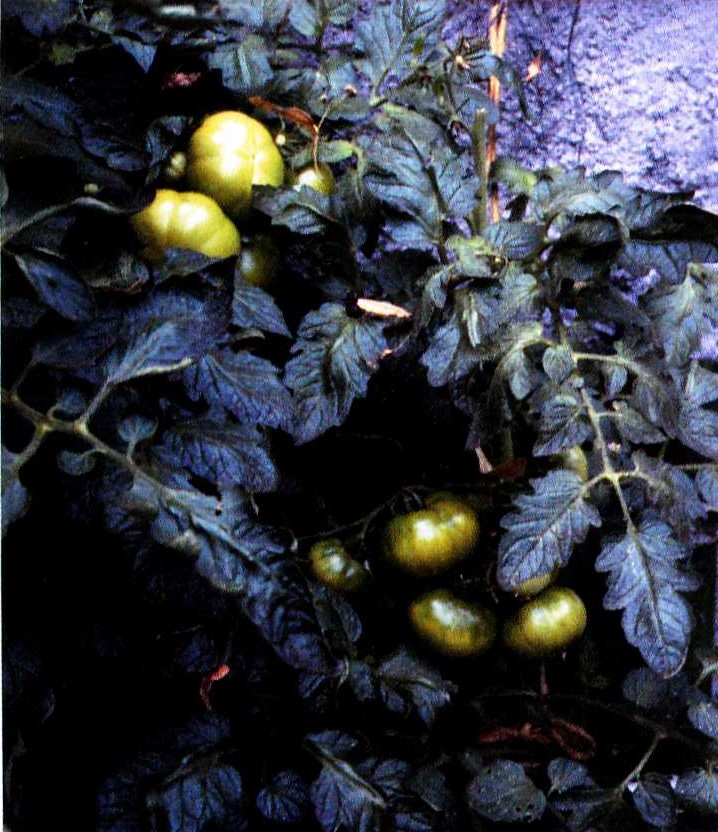
\includegraphics[width=0.4\textwidth]{bilder/nutzpfl_1.jpg}%
	\caption{Die Tomatenpflanze mit ihrem charakteristischen, verzweigten Aufbau\cite{nutzpflanzen}.}
	\label{tomaten_aufbau}
\end{wrapfigure}


Aus zwei verwachsenen Fruchtblättern, die aus mehreren Fächern bestehen und den Innenräumen entsprechen, setzt sich der Fruchtknoten zusammen \cite{Bluete, nutzpflanzen}. Dieser ist an einer zentralen Plazenta mit einigen Samenanlagen angebunden, die sich zu einem markreichen Gewebe im weiteren Verlauf entwickelt. In den Samenschalen befinden sich das sogenannte Myxotesta, welches sich als stark verschleimendes Zylinderepithel kennzeichnet (siehe Abbildung \ref{tomaten_both} rechts). Durch ein schleimiges Gewebe werden die Zwischenräume der Samen umschlossen, welches von der Plazenta abgesondert wird.


\begin{figure}[h!]
	\hfill
	\subfigure[]{
		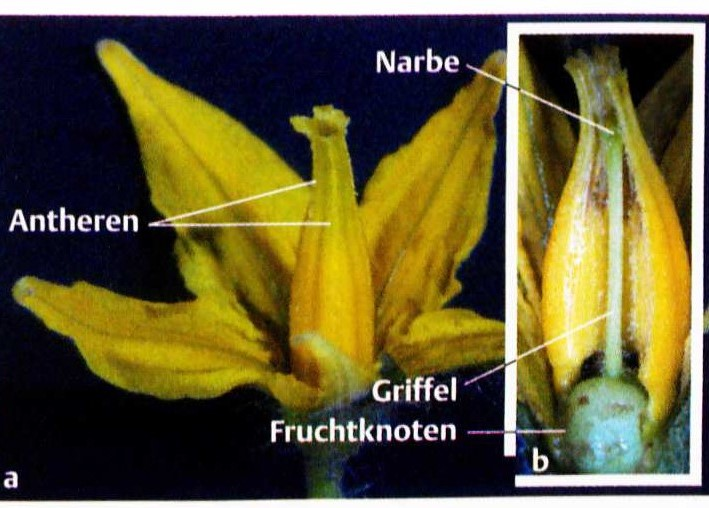
\includegraphics[width=0.45\textwidth]{bilder/nutzpfl_2a.jpg}}
	\hfill
	\subfigure[]{
		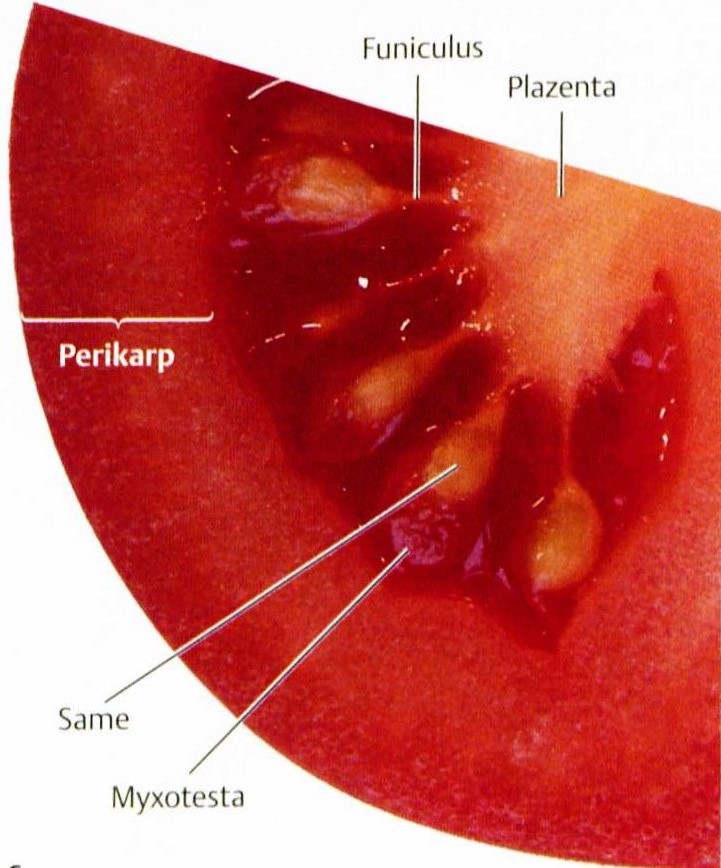
\includegraphics[width=0.45\textwidth]{bilder/nutzpfl_2b.jpg}}
	\hfill
	\caption{In der linken Darstellung wird die Blüte einer Tomate mit geöffneter Antherensäule veranschaulicht. Die rechte Abbildung zeigt einen Querschnitt der Frucht\cite{nutzpflanzen}.}
	\label{tomaten_both}
\end{figure}


\subsection{Anbau und Standortansprüche}



Aufgrund ihrer hohen Ansprüche und geringen Standfestigkeit benötigen Tomatenpflanzen, die an Pfählen oder hochgebundenen Seilen angebaut werden, bröckeligen, nährstoffreichen Boden. Da die Tomate ursprünglich aus den Tropen stammt\cite{nutzpflanzen}, können Kälteschäden auch bei Temperaturen über $0^\circ\text{C}$ auftreten. Deswegen werden Tomaten in Gewächshäusern gepflanzt, da sie dort nicht nur einen Schutz gegen die Kälte, sondern auch gegen Wind und Starkregen, erhalten. Außerdem werden für die Bestäubung der Pflanzen seit 1985 Hummeln (Bombus terrestris) ganzjährig eingesetzt. Hierfür werden diese speziell für den Tomatenanbau in Gewächshäusern gezüchtet.

\subsection{Wirtschaftliche Bedeutung}
%TODO: Quelle
%http://appsso.eurostat.ec.europa.eu/nui/submitViewTableAction.do einbauen

In diesem Abschnitt wird die wirtschaftliche Bedeutung von Tomaten betrachtet. Zunächst ist die Frage interessant, in welchen Mengen überhaupt in Deutschland Gemüse verzehrt wird. Anschließend werden die Erntemengen der europäischen Länder betrachtet.

\paragraph{Konsum von Tomaten}
~\newline

Der Verbrauch an Gemüse ist dank des statistischen Bundesamts\cite{bundesamt} klar dokumentiert. Die Abbildung \ref{pro_kopf_konsum} veranschaulicht in einem kleinen Ausschnitt den Pro-Kopf-Konsum in dem Zeitraum zwischen 2015 bis 2018 in Deutschland. Für vollständige Daten wird auf die Quelle verwiesen.

\begin{figure}[h!]
	\centering
	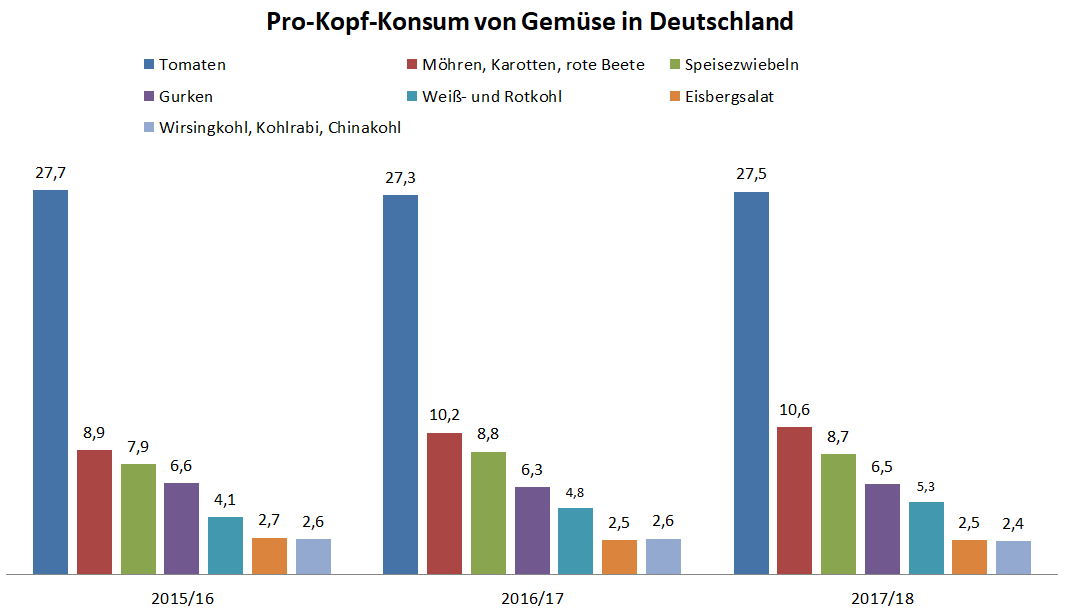
\includegraphics[width=\textwidth]{bilder/pro_kopf_konsum.PNG}
	\caption{Darstellung des Pro-Kopf-Konsums von Gemüse im Zeitraum 2015 - 2018\cite{bundesamt} (eigene Darstellung).}
	\label{pro_kopf_konsum}
\end{figure}

Auf der x-Achse sind einige Gemüsesorten als unterschiedlich gefärbte Säule aufgelistet. Auf der y-Achse befindet sich der Pro-Kopf-Konsum in Kilogramm. Keine andere Gemüsesorte wird so häufig konsumiert wie die Tomate. Mit 2281t (in 1000 Tonnen) liegt der Pro-Kopf-Konsum in dem Jahr 2017/18 bei 27.5kg. Bei anderen Gemüsesorten beispielsweise Möhren, Karotten und roten Rüben ist der Pro-Kopf-Konsum wesentlicher geringer und liegt bei 10.6kg. Dies entspricht der am zweithäufigsten konsumierten Gemüsesorte. Der kleinste Pro-Kopf-Konsum in der Abbildung beträgt 2.4kg und wird von Wirsingkohl, Kohlrabi und Chinakohl belegt.



\paragraph{Erntemenge in europäischen Ländern}
~\newline

Das Statistische Amt der Europäischen Union dokumentiert seit dem Jahr 2009 die Erntemenge in europäischen Ländern\cite{eurostat}. Hier wird nur ein kleiner Ausschnitt gezeigt. Das vorliegende Schaubild \ref{erntemenge} gibt Auskunft darüber, wie viele Tomaten in dem Zeitraum zwischen 2017 und 2018 in der Europäischen Union (inkl. Türkei) geerntet wurden. Dabei repräsentiert die x-Achse die Erntemenge in 1000 Tonnen. Auf der y-Achse werden die Länder angezeigt. Südländische Länder der EU, hier Italien, Spanien, Portugal und Griechenland, sind in dem Diagramm verstärkt vertreten. Italien erntet als europäisches Land im Jahr 2017 die meisten Tomaten mit 5573.31t (in 1000 Tonnen). In dem Zeitraum 2017 baut Rumänien die wenigsten Tomaten mit 435t (in 1000 Tonnen) an. Im Vergleich zum Jahr 2018 konnte die Erntemenge in den Ländern Italien, Polen, Griechenland und Rumänien gesteigert werden. Dennoch ist die Erntemenge in allen EU-Staaten in der Summe um $\approx$2\% gesunken. Die Erntemenge in der Türkei ist mindestens doppelt so groß als in Italien. Insgesamt entspricht die Erntemenge 73\% (2017) beziehungsweise 71\% (2018) der Gesamtsumme in der Europäischen Union. Angemerkt sei, dass nur ein Ausschnitt der Daten visualisiert wurde. Daten für alle 28 europäischen Länder sind in der Quelle abrufbar\cite{eurostat}.
	

\begin{figure}[h!]
	\centering
	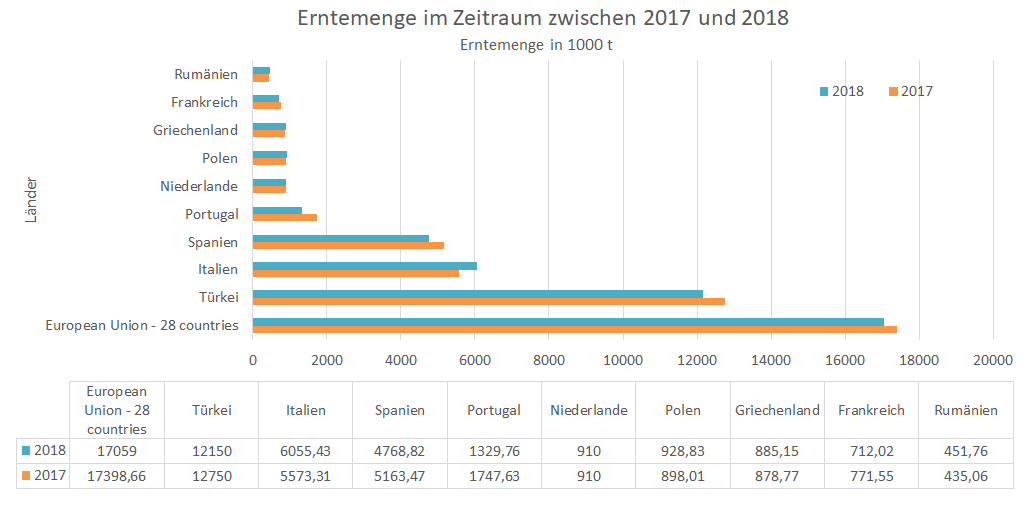
\includegraphics[width=0.9\textwidth]{bilder/erntemenge.PNG}
	\caption{Darstellung der Erntemenge\cite{eurostat} von europäischen Ländern in dem Zeitraum zwischen 2017 und 2018 (eigene Darstellung).}
	\label{erntemenge}
\end{figure}




\newpage
\section{Blattkrankheiten von Tomaten}
\label{sec:Blattkrankheiten}

Es existieren einige Pflanzenkrankheiten, die die Blätter von Tomaten angreifen können. Hier werden vier, nämlich die Dürrfleckenkrankheit, das TYLCV-Virus, die Samtfleckenkrankheit und die Krautfäule, mit ihren typischen Symptomen und Eigenheiten vorgestellt. 


\subsection{Dürrfleckenkrankheit}

%TODO: Sortieren!!! nicht abgeschlossen, \cite{solani}

Die häufigste Krankheit, welche von dem Pilz Alternaria solani verursacht wird, ist die Dürrfleckenkrankheit\cite{borner}. Diese Krankheit tritt besonders bei Tomaten auf und kann in Regionen, die starke Niederschläge, hohe Luftfeuchtigkeit sowie hohe Temperaturen bei $24^\circ-29^\circ\text{C}$ aufweisen, zu einer vollständigen Entlaubung führen. In überwiegend trockenen Klimazonen mit häufigen und anhaltenden, nächtlichen Tauen können sogar Epidemien auftreten. Des Weiteren greift der Pilz nicht nur die Blätter an, sondern zeigt auch Symptome an den Hauptstämmen der erwachsenen sowie jungen Tomatenpflanzen. Die Frucht selbst kann bei einem Befall faulen\cite{solani}. 


\subsubsection{Krankheitserreger}

Der Pilz Alternaria solani wurde zum ersten Mal von Ellis und Martin im Jahr 1882 als A. porri f. sp. solani beschrieben und gehört zu den Fungi imperfecti (Deuteromycotina) in der Klasse Hyphomycetes und Ordnung Hyphales. Alternaria solani gehört zu der Gruppe der großporigen Pilze, welche durch getrennte Konidien, die eine bestimmte Form von einer Spore ist, gekennzeichnet sind und auf einem einfachen Konidiophor getragen werden. Konidiophore bestehen aus fadenförmigen Zellen. Die Konidien von Alternaria solani sind dunkel und ellipsenförmig (s. Abbildung \ref{konidien}). Des Weiteren hat der Pilz mehrkernige und dunkel gefärbte Zellen. Die dunkle Farbe, die von Melanin gebildet wird, schützt den Pilz vor widrigen Umgebungsbedingungen und Mikroben\cite{solani}.

 
%TODO Bild an der richtigen Stelle bringen
\begin{figure}[h!]
	\centering
	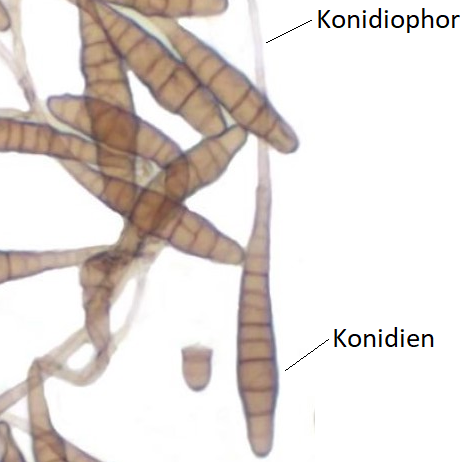
\includegraphics[width=0.7\textwidth]{bilder/konidien.png}
	\caption{In der Abbildung ist zu sehen, wie Konidien vom Erreger Alternaria solani aufgebaut sind. Der Körper des Erregers besteht aus mehreren Konidien in einer Kette gegliedert, welcher mit dem fadenförmigen Konidiophor verbunden ist\cite{konidien}.}
	\label{konidien}
\end{figure}

\subsubsection{Bekämpfung}

Ertragsverluste bis zu 79\% wurden aus Kanada, Indien, Nigeria sowie in den Vereinigten Staaten berichtet. Fäulnisse an dem Stammfuß können zu Verlusten (um die 20 - 40\%) von Keimlingen auf dem Feld führen. Erfolgreiche Bekämpfungsmaßnahmen gegen den Pilz sind beispielsweise Fungizide, die regelmäßig angewendet werden, sowie die Einsetzung von krankheitsfreien Jungpflanzen. Dabei zählt die Behandlung mit Fungiziden zu der wirksamsten Bekämpfungsmaßnahme, die aufgrund der Wirtschaftlichkeit nicht in allen Regionen der Welt durchgeführt wird und bei bestimmten Wetterkonditionen nicht effizient sein könnte. Resistente Sorten sind potenziell die wirtschaftlichste Bekämpfungsmaßnahme, da sie mit Fungiziden kombiniert werden können, um dabei die Kontrolle über den Pilz halten zu können. Allerdings ist die Züchtung von resistenten Pflanzen schwierig, da effektive resistente Gene in kultivierten Tomatenpflanzen kaum vorhanden sind\cite{solani}.

\subsubsection{Krankheitskreislauf}

Die Konidien keimen bei hoher Luftfeuchtigkeit beziehungsweise nahezu gesättigter Feuchtigkeit bei Temperaturen zwischen $8^\circ - 32^\circ\text{C}$ zu einem oder mehreren Keimrohren. Diese dringen anschließend in die Epidermal-Zellen oder durch Wunden aufgrund des Wachstums ein. Das Eindringen benötigt eine gewisse Temperaturspanne, die zwischen $10^\circ$ und $25^\circ\text{C}$ liegt. Die Zellwände des Wirts werden durch Enzyme, hier Cellulase und Pektinmethylgalacturonase, beschädigt, um Toxine abzulassen, die die Wirtszellen abtöten. Dadurch kann der Pilzerreger Nährstoffe aus den toten Zellen beziehen. Verletzungen von einer Infektion sind erst nach zwei bis drei Tagen sichtbar. Des Weiteren erfolgt die Produktion von Sporen ab dem dritten bis fünften Tag. Die Infektion selbst findet in einem sehr kurzen Zeitraum statt, so dass eine polyzyklische Infektion ermöglicht wird. Der Pilz überlebt als Konidien im Boden, in Pflanzenresten und in Samen. Weitere Überlebensmöglichkeiten des Erregers sind beispielsweise Chlamydosporen, welche durch die Zellteilung entstanden sind. Daher umfasst der Lebenszyklus von Alternaria solani den Boden-, Saatgut- und Luftbereich, so dass die Kontrolle des Erregers erheblich erschwert wird. Die Hauptwirte des Erregers sind Pflanzen aus der Familie der Nachtschattengewächse, beispielsweise Tomaten, Kartoffeln, Auberginen und Paprika\cite{solani}.

In der Abbildung \ref{solani_circle} wird der Krankheitszyklus veranschaulicht. Ausgehend von einer Infektion können Konidien in den Pflanzenresten und Samen überleben. Anschließend keimen Konidien, um die Zellwände entweder direkt zu durchdringen oder durch eine Wunde in das Zellinnere einzudringen. Bei dem Eindringen durch die Wunde werden die Früchte oder der Stamm infiziert. Das direkte Eindringen infiziert die Blätter der Pflanze, die Verletzungen auf Blättern, dem Stamm sowie der Frucht auslösen. Ausgehend von dieser Lage können neu produzierte Konidien die Pflanze erneut infizieren.  

\begin{figure}[h!]
	\centering
	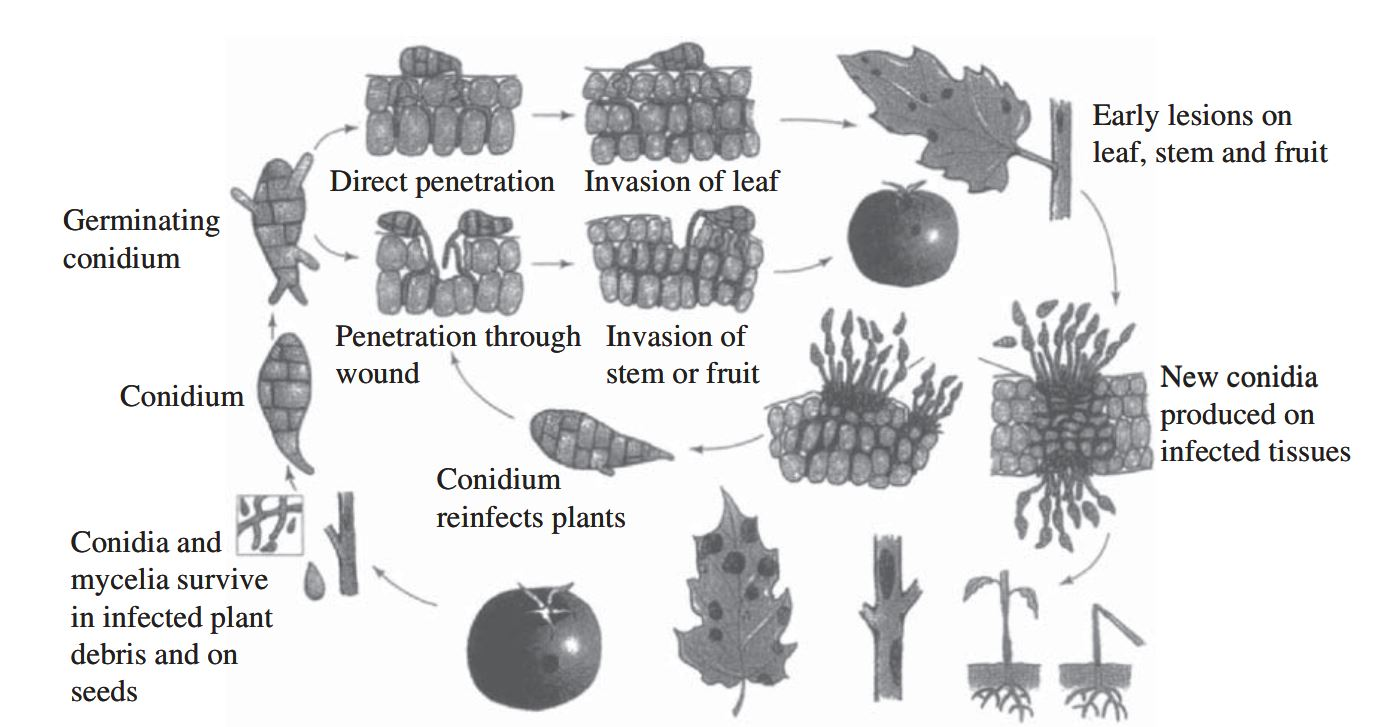
\includegraphics[width=\textwidth]{bilder/solani_circle.jpg}
	\caption{Darstellung des Krankheitskreislaufs mit einer polyzyklischen Struktur\cite{solani}.}
	\label{solani_circle}
\end{figure}


\subsubsection{Krankheitssymptome}

%todo Bild?

Alle oberirdischen Bestandteile der Pflanze können von Alternaria solani befallen werden und zeigen unterschiedliche Symptome an den Blättern, Früchten sowie Stämmen\cite{borner,solani}:

\begin{itemize}
	\item Dürrfleckenkrankheit: Die Symptome von dieser Krankheit bestehen aus kleinen, dunklen, nekrotischen Verletzungen auf den älteren beziehungsweise unteren Blättern. Mit zunehmendem Alter breitet sich die Krankheit zu den oberen Blätter aus. Die Verletzungen haben meist konzentrische Ringstrukturen, die oft von einer Vergilbungszone begleitet werden. Bei einer schweren Infektion sorgt Alternaria solani für ein vorzeitiges Absterben des Laubs, welches die Pflanze schwächt. Wegen der Schwächung können die Früchte durch Sonneneinstrahlungen verletzt werden. 
	 
	\item Fruchtfäule: Bei grünen oder reifen Früchten können am Stielende dunkle, versenkte Stellen auftreten. Der Auslöser dieser Stellen ist eine Stammverletzung, die eine beträchtliche Größe erreichen kann. Grundsätzlich sind halbreife Früchte anfälliger als reife. Des Weiteren fallen stark infizierte Früchte ab, bevor sie die Reifung erreicht haben. 
	
	\item Stammfäule: An den Hauptstielen und Seitenästen von erwachsenen Pflanzen verursacht der Pilz kleine, dunkle, leicht versunkene Stellen, die sich zu dunkelbraunen, länglichen Flecken vergrößern. Diese Vergrößerungen bilden konzentrierte Ringe, die auch auf den Blättern zu finden sind.
	
\end{itemize}




\subsection{Tomato Yellow Leaf Curl Virus}


In vielen tropischen und subtropischen Regionen weltweit stellt das Tomato Yellow Leaf Curl Virus (TYLCV) eine Bedrohung für die Tomatenproduktion dar\cite{TYLCV}. Am Ende der 1930er Jahre wurde von Schäden, die durch diese Krankheit verursacht wurden, berichtet. In Ländern des Nahen Ostens ist der Tomatenanbau von dieser Krankheit seit den 1960er Jahren stark betroffen. Die Ursache der Krankheit ist das Geminivirus, das einen zirkulären DNS-Einstrang hat und durch Insekten verbreitet wird\cite{gemini}. Mittels der weißen Fliege (Bemisia Tabaci), die als Vektor für diese Krankheit dient, wird diese Krankheit übertragen. Der B-Biotyp von Bemisia Tabaci ist seit den späten 1980er Jahren weltweit verbreitet. Dieser kennzeichnet sich durch ein breiteres Wirtsspektrum im Vergleich zu anderen Biotypen aus, so dass dieser nicht nur Unkraut oder Pflanzen, die geographisch auf ein bestimmtes Gebiet beschränkt sind\cite{endemic}, infiziert, sondern auch benachbarte nicht betroffene Kulturarten. Die TYLCV-Krankheit korreliert in tropischen und subtropischen Regionen in den letzten zehn Jahren mit den Ausbrüchen des B-Biototyps von Bemisia tabaci. Berichte aus dem Mittleren und Nahen Osten, Afrika, Europa und Mittelamerika vermerken Schäden an Tomatenkulturen, die auf die Virusart der TYLCV-Gruppe zurückzuführen sind. Das TYLCV-Virus wurde kürzlich in Japan, Mexiko sowie in Florida und Georgia in den Vereinigten Staaten von Amerika gemeldet. 

\subsubsection{Interaktionen zwischen dem Wirt und dem Virus}


Studien mit TYLCV-Is, TYLCV-Sar und verschiedene Quellen von Bemisia tabaci wurden durchgeführt, um Kenntnisse einer erfolgreichen Übertragung ermitteln zu können. Allerdings ist noch mehr Forschung notwendig, bevor die Mechanismen, die die Wechselwirkungen regeln, vollständig verstanden werden, um die Übertragung von Viren zu verhindern\cite{TYLCV}. 

Die minimale Übertragungszeit des Virus lässt sich in dem Intervall zwischen 17 bis 24 Stunden eingrenzen\cite{TYLCV}. Weibliche Fliegen sind anfälliger für das Virus als männliche und dienen daher vermehrt als Vektoren. Nymphen sind genau so anfällig wie Ausgewachsene, um das Virus zu bekommen. Mit steigendem Alter fällt die Anfälligkeit für eine Übertragung ab. Diese infektiösen weißen Fliegen können das Virus dann zehn bis zwölf Tage lang behalten und während der Nahrungsaufnahme in eine beliebige Anzahl gesunder Tomaten injizieren. Nach diesem Zeitraum müssen die Fliegen das Virus wieder erwerben, indem sie sich von einer infizierten Pflanze ernähren\cite{leaf_curl}. Des Weiteren ist das Virus für die weiße Fliege schädlich, da er auf die Lebenserwartung und Fruchtbarkeit einen Einfluss hat. Vermutlich kann sich das Virus in der Fliege reproduzieren. Allerdings wurde dies nicht bestätigt.


\subsubsection{Symptome}

Das Virus verursacht eine Krankheit, die bis zu einem totalen Gesamtertragsverlust führen kann\cite{leaf_curl}. Ihre Symptome lassen sich folgendermaßen beschreiben (s. Auflistung \ref{yellow_list}). Das Aufwärtsrollen der Blattränder ist das bekannteste Merkmal. Neben der Verkümmerung von Blättern sowie Blütenabstoßungen reduziert sich auch die Blattfläche und junge Blätter vergilben. Falls eine Infektion in frühem Wachstumsstadium vorliegt, dann ist der Verlust des Produktionsertrags fast absolut. Außerdem löst die Infektion den Rückgang des Pflanzenwachstums aus. Des Weiteren sollten bei der visuellen Diagnose von TYLCV mindestens zwei Symptome oder mehr vorliegen, um eine Fehldiagnose ausschließen zu können. Einzelne Symptome, zum Beispiel Blattvergilbung oder Blattkräuselung, können durch spezifische Umwelteinflüsse verursacht werden. 

\begin{itemize}
	\label{yellow_list}
	\item Blattvergilbung: Jüngere Blätter sind von einer Vergilbung des Blattes betroffen.
	
	\item Blattkräuselung: Das nach oben Aufrollen der Blattränder ist ein typisches Merkmal von TYLCV.
	
	\item Verkümmerung: Kombinationen von Viren können die Standfestigkeit der Pflanze reduzieren und eine verkümmelte Pflanze verursachen. 
	
	\item Blütenverlust: Der Verlust der ersten Blüte kann durch Umgebungsbedingungen oder leichte Ungleichgewichte in der Bodenfeuchtigkeit ausgelöst werden. Eine anhaltende Blütentrennung ist ein deutlicher Hinweis auf das TYLCV-Virus.
	
	\item Reduzierte Blattgröße: Neben der Verkümmerung von Blättern sowie Blütenverluste reduziert sich auch die Blattfläche.
\end{itemize}

\subsubsection{Verbreitung}


Für viele der Regionen, in denen das Virus sehr stark verbreitet ist, liegen nur begrenzte Informationen über TYLCV-Epidemien vor. Berichte über die natürliche Verbreitung des TYLCV-Virus auf der Grundlage groß angelegter Umfragen sind jedoch selten. Im Allgemeinen deuten die verfügbaren Daten darauf hin, dass das TYLCV-Virus in Unkrautwirten nicht weit verbreitet ist. In Ländern, zum Beispiel Spanien und Italien, verursacht das TYLCV-Sar Virus seit Ende der 1980er bzw. Anfang der 1990er Jahre schwere Epidemien bei Tomaten. Allerdings wurden nur die einjährigen Unkrautarten, hier D. stramonium, S. nigrum, S. luteum und Euphorbia sp., mit diesem Virus infiziert. Studien in Italien zeigten, dass sich das Auftreten von B. tabaci im Freien auf wärmere Regionen, in denen TYLCV-Epidemien auftreten\cite{TYLCV}, beschränkt. 


\subsection{Samtfleckenkrankheit}

Die Samtfleckenkrankheit tritt in manchen Regionen, zum Beispiel in Neuengland, nur in Gewächshäusern auf und befällt hauptsächlich Tomaten. Für den Ausbruch dieser Krankheit wird eine hohe Luftfeuchtigkeit beziehungsweise feuchte Pflanzenoberfläche benötigt\cite{Greenhouse}.


\subsubsection{Erreger}
Die Samtfleckenkrankheit, die erstmals von Cooke im Jahre 1883 beschrieben wurde \cite{Passalora}, wird von einem Pilzerreger, hier Cladosporium fulvum, verursacht, welcher auch unter dem Namen Passalora fulva beziehungsweise Fulvia fulva bekannt ist\cite{Cladosporium, leaf_mold}. Dieser zeichnet sich dadurch aus, nur Tomaten zu befallen\cite{leaf_mold}. Meistens sind die Blätter das einzige vom Pilz befallene Gewebe, dennoch können gelegentlich auch Stängel, Blüten, Stiele und Früchte befallen werden\cite{Passalora}.


\subsubsection{Symptome}

Von einer Infektion sind die ältesten Blätter zuerst betroffen. An den Oberseiten der Blätter bilden sich hellgrünlich-gelbe Flecken mit keinen ausgeprägten Rändern. Dabei sind die Flecken kleiner als 6,35 mm. Auf der unteren Blattfläche unterhalb der Blattflecken ist ein olivgrüner bis brauner Samtschimmel, zu erkennen (s. Abbildung \ref{samtflecken_bilder}). Des Weiteren können Blattflecken zusammenwachsen. Im weiteren Verlauf der Krankheit fangen die Blätter an, zu welken und zu sterben. Diese Blätter bleiben dennoch oft an der Pflanze hängen. Blüten, die auch infiziert sind, werden schwarz und fallen von der Pflanze ab. Bei einer Fruchtinfektion entstehen glatte, schwarze, unregelmäßige Fläche am Stammende der Frucht, die versenkt, trocken und ledrig werden\cite{Greenhouse, Passalora}. 


\begin{figure}[h!]

	\hfill
	\subfigure{
		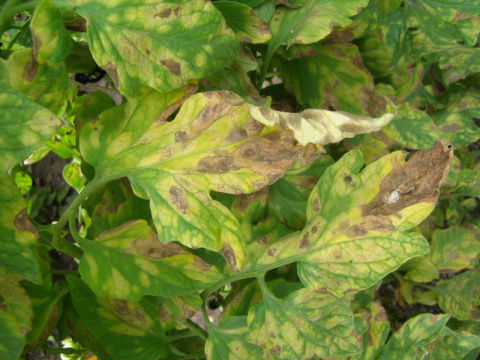
\includegraphics[width=0.45\textwidth]{bilder/upper-leaf-mold-tomato.jpg}}
	\hfill
	\subfigure{
		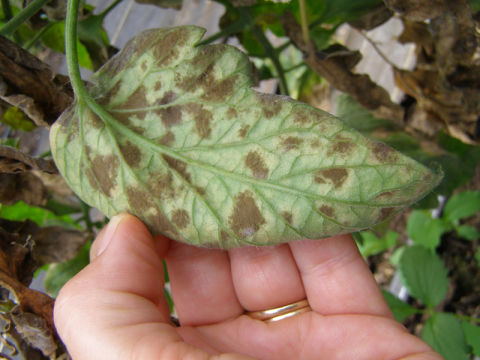
\includegraphics[width=0.45\textwidth]{bilder/leaf-mold-tomato-lower-spores.jpg}}
	\hfill
	\caption{In der linken Abbildung wird die Oberseite mit den hellgrünlich-gelbe Flecken visualisiert. Auf der unteren Seite des Blattes (rechte Abbildung) sind die einzelne Samtschimmelflecken klar zu erkennen\cite{leaf_mold}.}
	\label{samtflecken_bilder}
\end{figure}



\subsubsection{Krankheitsverlauf}

Sporen von dem Erreger können bei Zimmertemperatur auf dem Boden für sechs bis zwölf Monate überleben. Innerhalb der infizierten Pflanzenresten bildet der Erreger dunkle, harte Ruhestrukturen, in diese eine Menge neuer Sporen unter Lufteinwirkung produziert werden können. Durch diesen Mechanismus sichert sich der Erreger das Überleben von einer Jahreszeit zur nächsten. Des Weiteren kann der Erreger mittels Tomatensamen in ein anderes Gebiet eingeschleppt werden, weil er in und auf den Tomatensamen überleben kann.
Der optimale Temperaturbereich für eine Infektion, die von den Sporen ausgelöst wird, liegt zwischen 21$^\circ$ und 23$^\circ\text{C}$. Eine Luftfeuchtigkeit ab 85\% löst eine schwere Samtflecken-Epidemie aus. Dennoch kann diese Krankheit auch bei einer Luftfeuchtigkeit von weniger als 85\% auftreten. Die unteren Blätter der Pflanze sind bei der Infektion zuerst betroffen. Innerhalb eines Zeitraums zwischen zehn bis zwölf Tagen bilden sich neue Sporen auf der Unterseite der infizierten Blätter. Falls die Feuchtigkeit über 85\% bleiben sollte, dann können diese Sporen neue Blätter infizieren. Innerhalb der Anbauphase können mehrere Generationen des Erregers durch die Konidien von Blatt zu Blatt und von Pflanze zu Pflanze aufgrund von Wind, Regen und Insekten weiter verbreitet werden\cite{leaf_mold, Passalora, Greenhouse}.







\subsection{Krautfäule}

Weltweit ist die Krautfäule\cite{rapid_detect} als Erkrankung bei Kartoffeln und Tomaten bekannt. Vor dem Jahr 1992 wurden kaum Epidemien von Krautfäulen in den meisten Teilen der Vereinigten Staaten und Kanadas dokumentiert. Allerdings änderte sich dieser Zustand in den Jahren 1992 und 1993. Dieser Zeitraum zeichnete sich durch schwere Krautfäule sowohl auf Kartoffeln als auch auf Tomaten aus. Seit dem wird über die Krautfäule jährlich berichtet. Des Weiteren hindert die Krankheit in vielen Entwicklungsländern die Ausweitung des Kartoffelanbaus und sorgt jährlich für eine exzessive Anwendung von chemischen Fungiziden, die zu Resistenzen führt.  



\subsubsection{Erreger}
%QUELLE HINZUFÜGEN \cite{lbopat}lbopat hauptquelle


Die erste Entdeckung des Erregers\cite{lbopat} Phytophthora infestans wurde in den 1840er Jahren von M. J. Berkeley dokumentiert. Der Erreger gehört der Gruppe Oomycetes an und wird auch als Wasserschimmelpilz bezeichnet. Der Familienname für diese Gruppe von Organismen ist Peronosporaceae, die der Klasse Stramenopila der Eukaryonten zugeordnet werden. Die Pilze der Gruppierung Oomycetes sind keine echte Pilze, da sie mit den Braunalgen in enger Beziehung stehen. Der Zellkern beinhaltet einen doppelten Chromosomensatz (diploid), welcher für die meisten Pilzarten unüblich ist, da sie einen einfachen Chromosomensatz haben. 

An den Bildungsstätten von Sporen (Sporangien) bilden sich sackartige Strukturen auf den Sporangienträger (Sporangiophore), die für die asexuelle Reproduktion notwendig sind (s. Abbildung \ref{late_sack}). Die Sporangiophoren sind miteinander verbunden und produzieren kontinuierlich Sporangien. Durch diese stielartige Struktur werden Sporangien in der Luft verteilt. Der Erreger Phytophthora infestans gehört zu den wenigen Arten, die an eine solche Luftverteilung angepasst ist. Auch auf benachbarten Felder können Sporangien verteilt werden. Allerdings überleben die Sporangien aufgrund der Austrocknung und Sonneneinstrahlung in der Regel nicht. Falls die Felder unbehandelt sind, kann sich der Erreger dennoch von Feld zu Feld ausbreiten\cite{lbopat}.

\begin{figure}[h!]
	\centering
	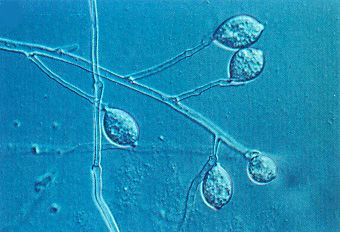
\includegraphics[width=0.7\textwidth]{bilder/LateBlight15.jpg}
	\caption{Darstellung der sackartigen Struktur, die mit dem Sporangienträger (Sporangiophore) verbunden ist\cite{lbopat}.}
	\label{late_sack}
\end{figure}

Unter bestimmten Umweltbedingungen reagieren Sporangien unterschiedlich. Unter wärmeren Bedingungen können Sporangien direkt keimen. Sporangien verhalten sich unter kühlen, nassen Bedingungen jedoch abweichend. Aus den Sporangien treten Zoosporen aus, die zwei Flagellen haben, um auf der Wirtspflanzenoberfläche schwimmen und die Pflanze infizieren zu können\cite{lbopat}.


\subsubsection{Symptome}
%https://cropwatch.unl.edu/potato/late_blights_description hinzufügen da selber inhalt

%\cite{lbopat,CropWatch}
Tomaten sowie Kartoffelpflanzen\cite{lbopat} sind anfällig für die Krautfäule. Die Blattsymptome zwischen Tomaten und Kartoffeln sind ähnlich und weisen nur minimale Unterschiede auf. Die Infektion mit der Krankheit kann wie bei den Kartoffeln schnell erfolgen. Die Bildung von weißen Sporen kann bei feuchtem Wetter erkennbar sein. Des Weiteren kann sich der Erreger in Stängeln sowie Tomatenblättern ausbreiten.

\begin{figure}[h!]
	\centering
	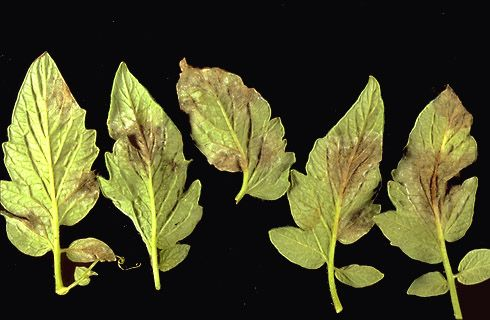
\includegraphics[width=0.7\textwidth]{bilder/LateBlight13.jpg}
	\caption{Infizierte Tomatenblätter weisen typische, dunkelbraune, feste Läsionen auf\cite{lbopat}.}
	\label{lateblight_leaves}
\end{figure}

Die Symptome einer Krautfäule-Infektion kennzeichnen sich durch dunkelbraune, feste Läsionen, die die gesamte Tomatenfrucht zerstören können. Läsionen an den Früchten werden mit leichter Fäulnis und einem Zerfall begleitet. Diese Symptome sind außerdem ähnlich bei den Kartoffeln. Die Abbildung \ref{lateblight_leaves} zeigt solche dunkelfarbige Verfärbungen auf den Blättern von Tomaten. 


\subsubsection{Krankheitskreislauf}

Der Erreger Phytophthora infestans überlebt als Myzel in den Tomatenfrüchten. Falls bei der Ernte infizierte Früchte zurückbleiben, können Sporangien auf den infizierten Früchten entstehen, die im folgenden Frühjahr die Krankheiten auslöst. Durch die Luftströmungen werden die Sporangien zu gesundem Blattlaub getragen und infizieren die Pflanzen. Frisch geschnittene Oberflächen sind besonders anfällig für Infektionen durch luftgetragene Sporen. Wenn ein infiziertes Saatgut gepflanzt wird, kann es zu einer lokalen Infektion kommen. Der Erreger breitet sich durch Bewegung in infiziertem Gewebe aus und die Vermehrung wird durch die asexuelle Reproduktion realisiert.

Außerdem können Sporangien indirekt durch die Produktion und Freisetzung von Zoosporen in Gegenwart von Wasser und bei kühleren Temperaturen keimen. Die direkte Keimung findet bei wärmeren Temperaturen statt. Hierbei bilden die Sporangien ein Keimrohr aus, an dem neue Sporangien entstehen. Grundsätzlich können sich die Sporangien durch Wind und Wasser in neue Teile der Pflanze beziehungsweise neue Pflanzen verbreiten\cite{lbopat}.%\cite{lateblightoverview, lbopat}

In der Abbildung \ref{diseasecircle_late} ist der Krankheitskreislauf veranschaulicht. Ausgehend von einer infizierten Pflanze befinden sich Sporen auf den Blättern, die in der Lage sind, Zoosporen freizusetzen und sich zu verteilen. Somit können weitere Pflanzen infiziert werden. Im Frühling können junge Pflanzen noch Sporen haben, die wiederum auch Zoosporen produzieren, um neue Pflanzen infizieren zu können.

\begin{figure}[h!]
	\centering
	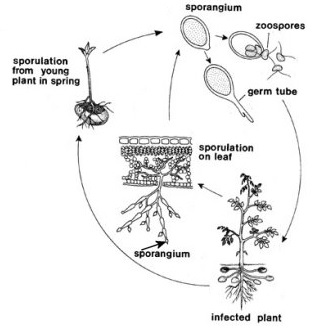
\includegraphics[width=0.7\textwidth]{bilder/LateBlightdiscycle_sm.jpg}
	\caption{Darstellung des Krankheitskreislaufs von der Krautfäule\cite{lbopat} (abgeändert).}
	\label{diseasecircle_late}
\end{figure}

\subsubsection{Verbreitung}
%\cite{lateblightoverview, lbopat}
Die wichtigsten Umweltfaktoren\cite{lbopat} bezüglich der Entwicklung von Krautfäule sind Temperatur sowie Feuchtigkeit und haben einen erheblichen Einfluss auf die Ausbreitung. Falls die relative Luftfeuchtigkeit unter 90\% liegt, dann bilden sich Sporangien auf den unteren Blattflächen und infizieren die Stängeln. Sporangien und Sporangiophore können bei Temperaturen um 3$^\circ$ bis 26$^\circ\text{C}$ auftreten. Der ideale Temperaturpunkt liegt bei 18$^\circ$ bis 22$^\circ\text{C}$. Zwischen 21$^\circ$ bis 26$^\circ\text{C}$ keimen Sporangien mittels eines Keimschlauches. Temperaturen, die unter 18$^\circ\text{C}$ liegen, sorgen dafür, dass Sporangien Zoosporen bilden, die zum Schwimmen Wasser benötigen. Jede einzelne Zoospore kann eine Infektion auslösen. Daher kann die Krankheit bei kühlen, nassen Bedingungen erheblich schwerer ausbrechen. Ganze Felder können bei kühlen Nächten und warmen Tagen unter zwei Wochen zerstört werden, da solche Umweltbedingungen optimal für eine Epidemie sind.



\subsubsection{Bekämpfung}
%\cite{rapid_detect, lateblightoverview}
Aufgrund des hohen Einsatzes von Fungiziden\cite{rapid_detect} sind Resistenzen entstanden, so dass die Einpflanzung von gegen den Erreger resistenten Tomatenpflanzen erheblich erschwert wurde. Infizierte Tomaten lassen sich daher effektiv folgendermaßen bekämpfen\cite{lbopat}:

\begin{itemize}
	\item \textbf{Standortwahl}: Eine gute Entwässerung und Luftzirkulation reduzieren die Luftfeuchtigkeit. Allerdings dürfen Felder, die von Bäumen und einer dichten Vegetation begrenzt werden, nicht benutzt werden. 
	
	\item \textbf{Fruchtfolge}: Zur Bekämpfung der Krautfäule können Rotationen des Feldes von zwei bis drei Jahren stattfinden. Hierbei werden Kulturen verwendet, die für den Erreger nicht als Wirt geeignet sind. Des Weiteren werden nicht nur Kartoffeln und Tomaten von dem Erreger infiziert, sondern auch weitere Nachtschattengewächse.
\end{itemize}

In der Quelle\cite{lbopat} sind weitere Bekämpfungsmaßnahmen bezüglich der Bekämpfung bei Kartoffeln aufgelistet.



\chapter{Maschinelles Lernen}
\label{sec:machine_learning}
%TODO: Deutsche Begriffe, Quelle: introml

Der Bereich \glqq Maschinelles Lernen\grqq~(engl. machine learning) beschäftigt sich mit Algorithmen und Techniken zur Automatisierung von Lösungen für komplexe Probleme, die mit konventionellen Programmiermethoden schwierig umsetzbar sind. Bei der herkömmlichen Programmiermethode werden zwei verschiedene Schritte durchgeführt. Zunächst wird die Spezifikation des Programms bestimmt, um einen detaillierten Entwurf des Programms erstellen zu können. Hierbei werden Fragen, zum Beispiel \glqq Was soll das Programm können\grqq, beantwortet. Der nächste Schritt ist die Implementierung des Entwurfs mittels einer Programmiersprache\cite{IntroML}.

Die Problematik an diesem Ansatz ist, dass viele reale Probleme mit der konventionellen Methode trotz des detaillierten Entwurfs schlecht dargestellt werden können. Das Erkennen von handgeschriebenen Zeichen in einem Bild ist ein bekanntes Beispiel für diese Problematik. Der Datensatz, der aus einer großen Menge von handgeschriebenen Zeichen besteht, wird zusätzlich zu jedem Bild mit einem Label versehen, welches das handgeschriebene Zeichen wiedergibt. Letztendlich beschreibt der beschriftete Datensatz, wie sich das Programm verhalten soll. Hierbei ist das Ziel ein Programm zu entwickeln, welches die Zeichen in jedem neuen Bild erkennen soll. Dabei soll die Erkennung auch funktionieren, wenn die Bilder nicht im Datensatz vorkommen. Mit der herkömmlichen Methode wird ein allgemeiner Satz von Regeln aufgestellt, die die Beziehung zwischen den Bildern und den Zeichen beschreibt. Aufgrund der großen Unterschiede bei den handgeschriebenen Schriftzeichen kann ein solches Regelwerk eine große Herausforderung sein\cite{IntroML}.

Diese Probleme lassen sich mittels ML-Algorithmen auf einer generischen Weise lösen. Hierbei verlangen solche Algorithmen keine detaillierte Beschreibung, wie der Entwurf aussehen muss. Sie erlernen stattdessen den detaillierten Entwurf aus einem Satz von beschrifteten Daten, die das Verhalten des Programms repräsentieren. Hierbei erstellt der ML-Algorithmus ein Modell, welches er aus den beschrifteten Daten gelernt hat\cite{IntroML}.
\newpage

Da dieser Bereich in vier große Teilgebiete unterteilt werden kann, werden diese kurz vorgestellt\cite{francois}:

\begin{itemize}
	\item Unüberwachtes Lernen
	\item Überwachtes Lernen
	\item Selbstüberwachtes Lernen
	\item Bestärkendes Lernen
\end{itemize}

\section{Unüberwachtes Lernen}
%BOOK i francois

Dieser Teilbereich des maschinellen Lernens befasst sich damit, interessante Informationen aus den Eingabedaten zu ermitteln, ohne die notwendigen Labels zu benötigen. Dies kann die Visualisierung, Erfassung sowie Verarbeitung von Daten erleichtern, da sie Zusammenhänge, die in den Daten gegeben sind, besser darstellen kann. Daher ist das unüberwachtes Lernen ein notwendiger Schritt, um den Datensatz besser verstehen zu können. Dimensionalitätsreduktion und Clustering sind bekannte Anwendungen aus dem Bereich des unüberwachtes Lernens\cite{francois}.

\begin{figure}[h!]
	\centering
	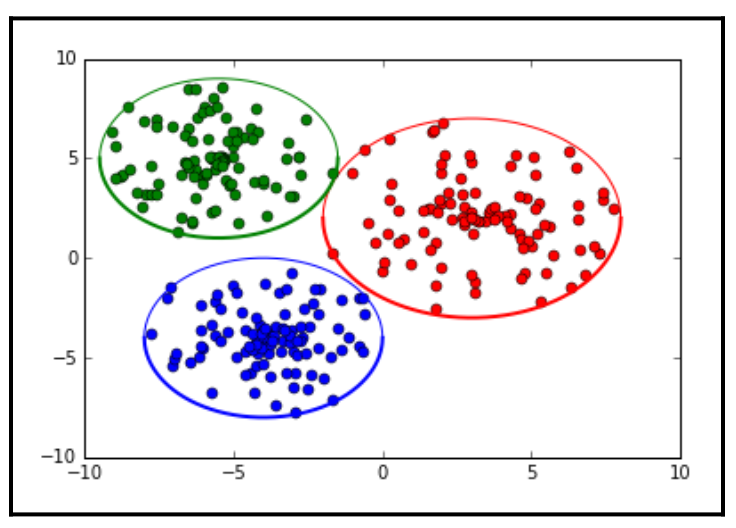
\includegraphics[width=0.7\textwidth]{bilder/cluster.PNG}
	\caption{Drei verschiedene Cluster mit den jeweiligen ähnlichen Datenpunkten werden in drei unterschiedlichen Farben visualisert\cite{Vasilev2019}.}
	\label{cluster}
\end{figure}


Beim Clustering erhält der Algorithmus eine Menge an Daten, die er in eine oder mehrere separate Gruppen (engl. Clusters) einteilt. Hierbei wird die Zuordnung der Daten anhand einer Metrik bestimmt, um die Ähnlichkeit der Daten innerhalb einer Gruppe zu maximieren sowie die Ähnlichkeit der Daten zwischen verschiedenen Gruppen zu minimieren. Dabei können Algorithmen auf verschiedene Metriken zurückgreifen, um die Ähnlichkeit messen zu können\cite{Vasilev2019}. In der Abbildung \ref{cluster} sind drei farblich unterschiedliche Gruppen zu sehen, in denen Datenpunkte ähnlich zueinander sind.




\section{Überwachtes Lernen}
%todo: deep learning erklären
Der häufigste Anwendungsfall\cite{francois} des maschinellen Lernens fällt unter dieser Kategorie. Das Ziel des überwachten Lernens (engl. supervised learning) ist das Erlernen der Zuordnung von Eingabedaten zu bekannten Ziele (engl. labels) anhand einer Menge von Beispielen. Diese Beispiele werden von Menschen erstellt. Das Lernverfahren ist daher unter menschlichem Einfluss gesteuert\cite{MLkurz}. Das erlernte System wird auf unbekannte Daten angewendet, um die Labels von bisher nicht bekannten Daten vorhersagen zu können. Die mathematische Funktion, die beim Lernverfahren gelernt werden soll, soll optimiert werden, so dass die Parameter der Funktion korrekt die bekannten Daten wiedergeben sowie unbekannte Daten vorhersehen können\cite{MLkurz}.
Fast alle Anwendungen, zum Beispiel Spracherkennung, Bildklassifizierung, Sprachübersetzung und Texterkennung, gehören zu dieser Kategorie und bestehen hauptsächlich aus Klassifizierung und Regression. Dennoch existieren einige Varianten, die nicht offensichtlich als Klassifizierung und Regression erkennbar sind. Beispiele\cite{francois} hierfür sind:

\begin{itemize}
	\item Sequenzgenerierung: Zu einem gegebenen Bild soll eine Beschriftung vorhergesagt werden, die das Bild beschreibt. Dabei kann die Sequenzgenerierung aufgrund der wiederholenden Klassifizierung eines Wortes in der Sequenz als eine Reihe von Klassifizierungsproblemen angesehen werden.
	
	\item Syntaxbaumvorhersage: Zu einem gegebenen Satz wird eine Zerlegung in einen Syntaxbaum prognostiziert.
	
	\item Objekterkennung: Bei diesem Problem wird ein minimaler Hüllkörper (engl. bounding box) um ein bestimmtes Objekt in einem gegebenen Bild gezeichnet. Als Klassifikationsproblem können die Inhalte der Hüllkörper bestimmt werden. Bei einem Regressionsproblem werden die Koordinaten des Hüllkörpers in Form eines Vektors bestimmt. 
	
	\item Bildsegmentierung: Bestimmte Objekte können mit einer pixelbasierten Maske im Bild maskiert werden.
	
\end{itemize}


\subsection{Selbstüberwachtes Lernen}

Das selbstüberwachte Lernen (engl. self-supervised learning) ist ein spezieller Fall des überwachten Lernens. Der Unterschied liegt darin, dass das Verfahren ohne von Menschen erstellten Labels arbeiten kann. Die benötigten Labels werden aus den Eingabedaten mithilfe eines heuristischen Algorithmus generiert. Bekannte Beispiele für das selbstüberwachte Lernen sind Autoencoder, dessen zu lernende und generierte Ziele die Eingabedaten sind. Autoencoder werden beispielsweise benutzt, um das nächste Einzelbild (engl. Frame) anhand von vergangenen Einzelbildern in einer Videosequenz vorherzusagen. Analog besteht die Möglichkeit, das nächste Wort in einem gegebenen Text zu prognostizieren\cite{francois}. 



\subsection{Bestärkendes Lernen}
%book f, francois, C
%theoretisch sehr viel mit quelle h

Durch das erfolgreiche Erlernen von Atari-Spielen sowie Go mittels Google DeepMind erlangte das verstärkende Lernverfahren (engl. reinforcement learning) sehr viel Aufmerksamkeit. Bei diesem Lernverfahren erhält ein Agent Informationen über seine Umgebung, um eine bestmögliche Aktion auswählen zu können. Dabei versucht er Belohnungen zu einer bestimmten Aktion zu maximieren. Zum Beispiel kann ein neuronales Netz, welches das aktuelle Einzelbild betrachtet, Spielhandlungen vorschlagen, um seine Punktzahl zu maximieren\cite{francois,Vasilev2019}. Ein solches Szenario kann mit einem verstärkenden Lernverfahren trainiert werden. Derzeit ist das Verstärkungslernen vor allem ein Forschungsgebiet und hat noch keine nennenswerten praktischen Erfolge außerhalb von Spielen erzielt. Dennoch kann dieses Verfahren im Laufe der Zeit auf Anwendungsgebiete aus der Praxis, beispielsweise selbstfahrende Autos, Robotik, Ressourcenmanagement, Bildung, ect., einen signifikanten Einfluss haben\cite{francois}.

\section{Künstliche neuronale Netze}
%BOOK 978


Die Vorbilder von künstlichen neuronalen Netzwerken sind die parallelen Strukturen von tierischen Gehirnen\cite{Bell2014}. Auf einer einfachen Form von Ein- und Ausgängen basiert grundsätzlich das Netzwerk. Aus biologischer Sicht besteht ein Neuron aus einer Zelle, welches in der Lage ist, chemische oder elektrische Signale zu verarbeiten sowie zu übertragen. Ein typisches Netzwerk setzt sich mit Neuronen zusammen, die miteinander verbunden sind. Im menschlichen Körper existieren Milliarden von Neuronen, die sich ein dichtes Netzwerk von Verknüpfungen bilden. Ein solches Neuron besteht aus drei Bestandteilen, nämlich der Eingang, welcher auch Dendrit genannt wird, der Zellkörper und der Ausgang, der als Axon bezeichnet wird. Dieser Aufbau ist in der Abbildung \ref{neural_human} veranschaulicht. 

\begin{figure}[h!]
	\centering
	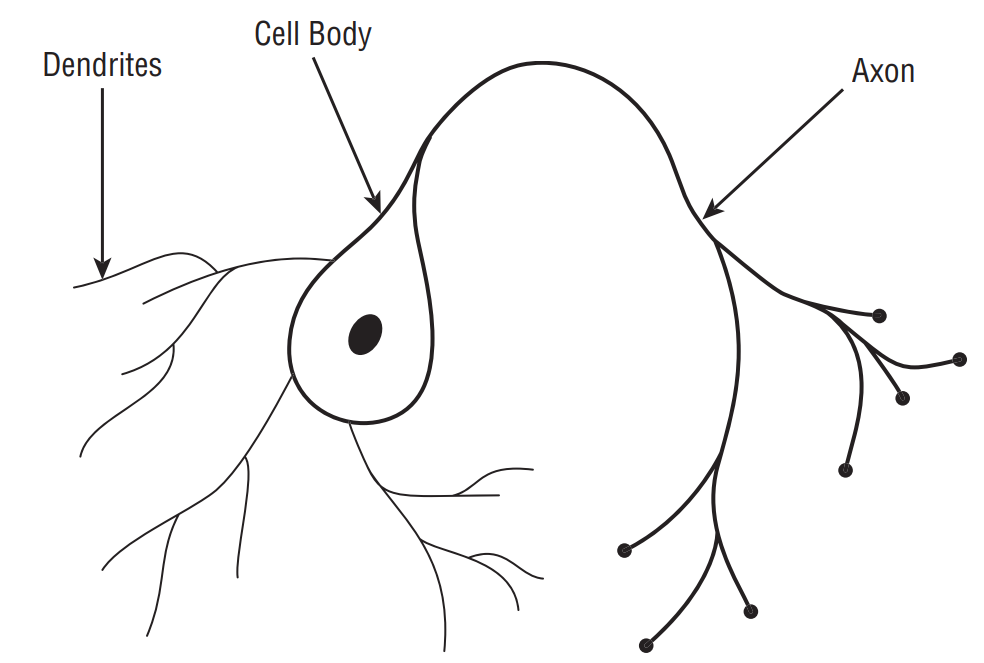
\includegraphics[width=0.7\textwidth]{bilder/neural_human.PNG}
	\caption{Vereinfachte Darstellung eines Neurons, welches aus einem Zellkörper mit den jeweiligen Ausgängen besteht\cite{Bell2014}.}
	\label{neural_human}
\end{figure}

Die Ausgänge eines Neurons werden mit den Eingängen von anderen Neuronen verknüpft, so dass ein Netzwerk aus Verknüpfungen entstehen kann. Die Komplexität von biologischen Gehirnen ist recht hoch und können bei einem Neuron 10000 verschiedene Eingänge haben. Des Weiteren werden Neuronen aktiviert, wenn das elektrochemische Signal durch das Axon gesendet wird. Das Signal erhält von dem Zellkörper eine Gewichtung. Falls ein Schwellenwert überschritten werden sollte, wird der Befeuerungsprozess durch den Ausgang entlang des Dendriten weitergeführt\cite{Bell2014}.

\subsection{Aufbau von neuronalen Netzen}
% book d Nelli2018

Die Strukturen von künstlichen neuronalen Netzen sind komplex aufgebaut. Dennoch basiert die Struktur auf einfacher grundlegender Bausteine, die innerhalb der Struktur wiederholt werden. Dadurch können komplexe Netzwerke beziehungsweise Architekturen, die von der Anzahl der grundlegenden Bausteine sowie den Typen der Verbindungen abhängig sind, entstehen, die besondere Merkmale hinsichtlich der Lernfähigkeit und der Lösung verschiedener Probleme aufweisen können. In der Abbildung \ref{network_aufbau} symbolisieren die farbigen Kreise die Basiseinheit, die auch als Knoten bezeichnet wird. Diese simulieren im biologischen Modell die Funktionalität eines Neurons in einem neuronalen Netzwerk und führen sehr einfache Operationen durch. Die Aktivierung der künstlichen Neuronen erfolgt dann, wenn die Gesamtsumme der empfangenen Eingangssignale einen bestimmten Schwellwert überschreitet. Des Weiteren können Signale zwischen den Knoten mittels Verbindungen, auch Kanten genannt, übertragen werden. Diese Verbindungen sollen die Funktionalität von biologischen Synapsen nachbilden, die in derselben Abbildung als blaue Pfeile dargestellt werden. Die Idee dahinter ist, dass das gesendete Signal von einem zu dem nächsten Neuron übertragen wird und gleichzeitig als ein Filter wirkt. Somit wandelt jede Kante, die eine Gewichtung bezüglich der Intensität hat, das Ausgangssignal eines Neurons entweder in ein hemmendes oder erregendes Signal um. Es existiert im neuronalen Netzwerk eine bestimmte Anzahl von Neuronen, die das Eingangssignal von außen annehmen können und sich in der linken Spalte in dem Netzwerkschema befinden. Diese Spalte stellt die sogenannte Eingangsschicht (engl. input layer) eines neuronalen Netzes dar (s. Abbildung \ref{network_aufbau}). In Abhängigkeit von den empfangen Eingangssignalen werden einige Neuronen aktiviert, weil das empfangene Signal verarbeitet und das Ergebnis an die andere Gruppe von Neuronen über die Kanten weitergeleitet wird. Als versteckte Schicht wird die zweite Gruppierung genannt, da sie sich zwischen dem Eingang und dem Ausgang befindet und von der nicht vorhanden Kommunikation im Eingang sowie im Ausgang mit der Außenwelt abgeschottet sind. In derselben Abbildung werden die eingehenden Kanten in der versteckten Schicht veranschaulicht, die mit allen Neuronen der vorherigen Schicht verbunden sind. Die Aktivierung der versteckten Neuronen erfolgt wie bei allen anderen Neuronen durch die Überschreitung des Schwellwerts. Nach der erfolgreichen Übertragung des Signals wird dieses verarbeitet und entweder an eine weitere Gruppe von versteckten Neuronen oder an die Ausgabeschicht (engl. output layer), die die Ergebnisse nach außen sendet, übertragen. Durch den allgemeinen Aufbau ist der Datenfluss stets von links dank der Eingabeschicht nach rechts zu der Ausgabeschicht. Letztendlich beruht die Effizienz und das Verhalten eines neuronalen Netzes auf den verbundenen Knoten, deren Verbindungen sowie die Anzahl der Schichten\cite{Nelli2018}.  


\begin{figure}[h!]
	\centering
	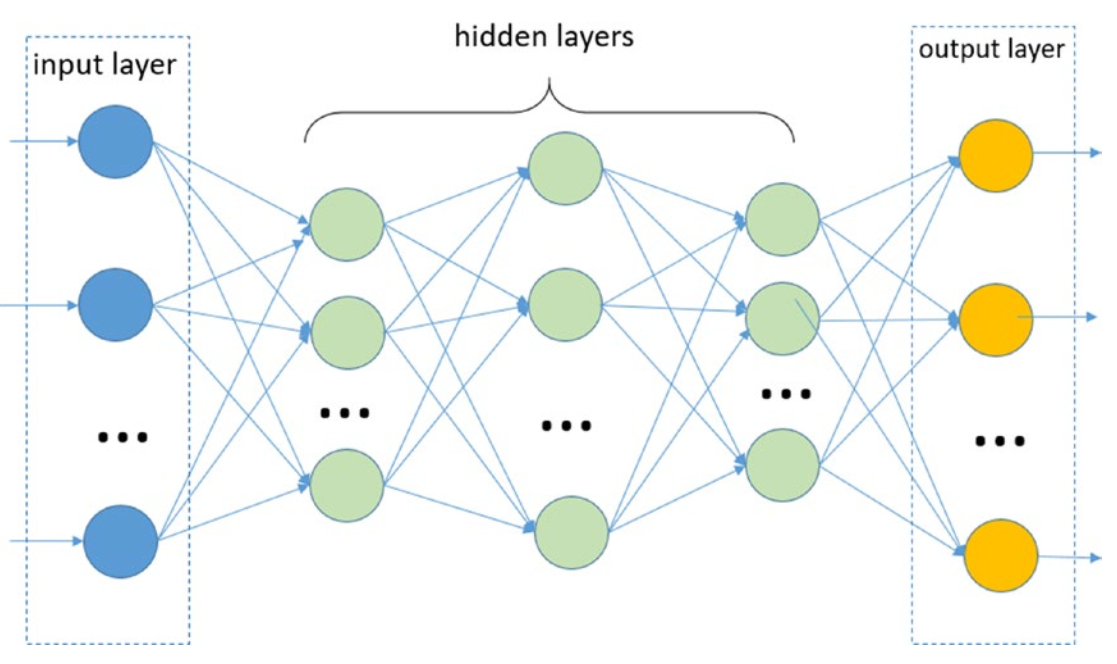
\includegraphics[width=\textwidth]{bilder/network_aufbau.PNG}
	\caption{Die Darstellung zeigt, wie ein generisches künstliches neuronales Netzwerk schematisch aufgebaut ist\cite{Nelli2018}.}
	\label{network_aufbau}
\end{figure}


\subsection{Einschichtiges Perzeptron}
%Book D \cite{Nelli2018}.

Im Jahre 1958 wurde das einfachste Modell eines neuronalen Netzes\cite{Nelli2018}, auch einschichtiges Perzeptron (engl. Single Layer Perceptron) genannt, von Frank Rosenblatt entworfen. Die Architektur ist in der Abbildung \ref{single_perz} veranschaulicht. 

\begin{figure}[h!]
	\centering
	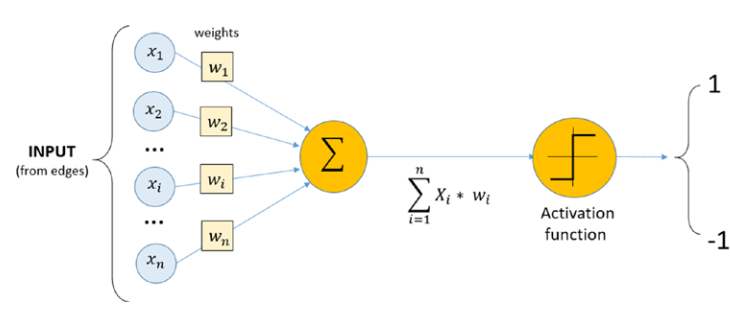
\includegraphics[width=\textwidth]{bilder/single_perz.PNG}
	\caption{Darstellung der Architektur von einem einschichtigen Perzeptron\cite{Nelli2018}.}
	\label{single_perz}
\end{figure}

\newpage
Das Modell besteht aus einer Eingabeschicht mit einer Anzahl von Neuronen, die ihre Signale mit einem Gewicht versehen und anschließend an das einzelne Neuron versenden. Die Funktionsweise des mathematischen Modells lässt sich folgendermaßen erklären. Zunächst werden die Kanten durch einen Gewichtsvektor $W$ repräsentiert:

\begin{equation}
	W = (w_1, w_2, ... , w_n)
\end{equation}

Anschließend empfängt das Ausgangsneuron ein Eingangsvektorsignal $x_i$, welches jeweils von einem anderen Neuron übermittelt wird.

\begin{equation}
X =(x_1, x_2, ... , x_n)
\end{equation}

Anschließend verarbeitet das Ausgangsneuron die Eingangssignale über eine gewichtete Summe.

\begin{equation}
	\sum_{i = 1}^{n} w_i x_i = w_1x_1 + w_2x_2 + ... + w_nx_n = s
\end{equation}

Das resultierende Signal s, welches vom Ausgangsneuron wahrgenommen wird, kann das Ausgabeneuron aktivieren, wenn es den Aktivierungsschwellenwert überschritten hat und sendet den Wert 1. Bei einer nicht erfolgreichen Aktivierung bleibt das Neuron inaktiv und verschickt den Wert -1.

\begin{equation}
\label{sp_activation}
	\text{Ausgabe} = 
	\begin{cases}
	1, & \text{wenn s$>$0}\\
	-1, & \text{sonst}
	\end{cases}
\end{equation}

Die Gleichung \ref{sp_activation} zeigt die einfachste Aktivierung. Es existieren weitere Aktivierungsfunktionen, die im Abschnitt \ref{aktivierungsfunktionen} vorgestellt werden.



\subsection{Aktivierungsfunktionen}
\label{aktivierungsfunktionen}
%TODO: Quellen!
%Book 129 \cite{Gonzalez2018}

Aus mehreren miteinander verbundenen Perzeptron-ähnlichen Einheiten besteht das neuronale Netz. Allerdings existieren Unterschiede zwischen eines neuronalen Netzes und eines Perzeptrons, wie sie das Ergebnis eines Signals verarbeiten. Die vorherige Abbildung \ref{single_perz} zeigt ein Perzeptron, welches eine Schwellenwertfunktion hat. Diese Funktion kann lediglich nur zwei Werte ausgeben, nämlich -1 und +1. Mit diesen zwei Werten führt das Perzeptron eine Klassifizierung durch. Anhand eines Beispiels lässt sich das Verhalten der Schwellenwertfunktion von einem Netzwerk aus Perzeptronen illustrieren. Angenommen, in diesem Netzwerk ist die Ausgabe vor dem Schwellenwert einer der Perzeptronen winzig klein und größer als null. Wenn der Schwellenwert erreicht wird, wird dieses sehr kleine Signal in ein +1 umgewandelt. Dennoch kann ein ähnlich kleines Signal mit dem entgegengesetzten Vorzeichen zu großem Wertumschwung von +1 nach -1 führen. Da neuronale Netze aus Schichten von Knoteneinheiten gebildet werden, bei denen die Ausgabe eines Knotens das Verhalten aller ihr folgenden Knoten beeinflussen kann, führt diese Empfindlichkeit gegenüber kleiner Signale zu Stabilitätsproblemen. Deswegen sind Perzeptronen für diese Architektur ungeeignet. Diese Problematik lässt sich lösen, in dem die Aktivierungsfunktion von einem hart beschränkten auf eine glatte, sanfte Funktion verändert wird\cite{Gonzalez2018}. Die bekannteste Aktivierungsfunktion ist die sogenannte Sigmoid-Funktion:

\begin{equation}
\label{sigmoid}
	h(z) = \frac{1}{1 + \exp(-z)}
\end{equation}

Die Variable $z$ entspricht der Summe eines berechneten Neurons. Der Vorteil an solchen glatten Funktionen liegt darin, dass sie leicht ableitbar sind.

\begin{equation}
\label{ableitung_sig}
	h'(z) = \frac{\partial h(z)}{\partial z} = h(z)[1 - h(z)]
\end{equation}


Die Abbildung \ref{aktivierung} zeigt drei verschiedene Aktivierungsfunktionen, die sehr häufig im Kontext des neuronalen Netzes verwendet werden. Der linke Graph entspricht der von der Gleichung \ref{sigmoid} bekannten Sigmoid-Funktion. Diese hat eine gestauchte S-Form und die Funktionswerte befinden sich zwischen 0 und 1. Im Vergleich zu der hyperbolischen Tangensfunktion hat diese Funktion keine starke Stauchung der S-Form. Des Weiteren sind die Funktionswerte im Bereich zwischen 1 und -1. Die rechte Funktion ist die ReLU-Funktion (Rectifier linear unit). Diese zeichnet sich aus, negative Eingabewerte auf den Wert null zu normieren. Des Weiteren neigt diese Funktion dazu, bessere Leistungen bei tiefen neuronalen Netze zu zeigen\cite{Gonzalez2018}.

\begin{figure}[h!]
	\centering
	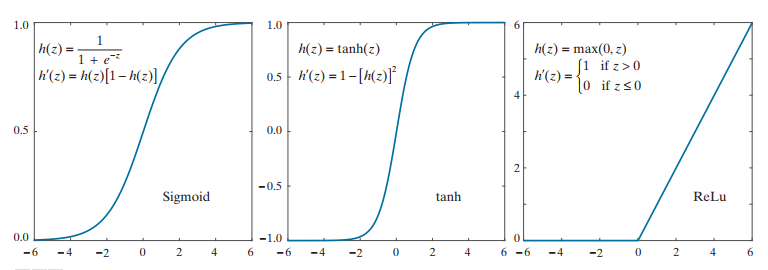
\includegraphics[width=\textwidth]{bilder/aktivierung.PNG}
	\caption{Hier sind drei Aktivierungsfunktionen zu sehen. Die linke Abbildung veranschaulicht die Sigmoid-Funktion. Anschließend folgt die hyperbolische Tangensfunktion. Die letzte Abbildung ist die sogenannte ReLU-Funktion \cite{Gonzalez2018}.}
	\label{aktivierung}
\end{figure}

\newpage
Weiterhin existieren weitere Aktivierungsfunktionen, die hier kurz beschrieben werden\cite{Vasilev2019}:

%book h
\begin{itemize}
	\item Identitätsfunktion: $f(a) = a$ \newline Diese Funktion bewirkt, dass der Aktivierungswert unverändert durchlaufen wird. 
	
	\item Schwellenwertaktivitätsfunktion: f(a) = 
	$\begin{cases}
		1, & \text{wenn a$\geq$0}\\
		0, & \text{wenn a$<$0}
	\end{cases}$
	\newline Wenn die Aktivierung über einem bestimmten Wert liegt, dann aktiviert diese Funktion das Neuron.
	
	\item bipolare Sigmoid-Funktion: $f(a) = \frac{1-\exp(-a)}{1+\exp(-a)}$ \newline Diese Funktion entspricht der stochastischen Sigmoid-Funktion, die neu skaliert und verschoben wurde, um den Wertebereich zwischen -1 und 1 zu erhalten.
	
\end{itemize}


\subsection{Lernverfahren}

Da die Gewichte der Kanten noch unpassend sind, müssen neuronale Netze dementsprechend diese lernen. Auf iterative Weise lernt das neuronale Netz. Hierbei wird eine Anzahl von Zyklen durchgeführt, um die Gewichte der Kante leicht verändert anpassen zu können. Jeder Lernzyklus entspricht einer Epoche. Für das Lernverfahren werden Eingabedaten, auch Trainingsdaten genannt, benötigt. Für jeden Eingangswert wird der erwartete Ausgangswert ermittelt, um einen Vergleich mit dem Ausgabewert, welcher von dem neuronalen Netz stammt, durchzuführen. Die Differenz zwischen den Eingabewerten sowie den erzeugten Ausgabewerten ist die Grundlage für die Veränderung der Gewichtswerte. Mithilfe einer Kostenfunktion, die das Ziel einer Minimierung hat, werden die Gewichte der verschiedenen Kanten für jede Epoche angepasst. Nach Abschluss der Lernphase folgt die Evaluierungsphase. In dieser Phase wird das trainierte neuronale Netz einen anderen Satz von Eingabewerten, hier Testdatensatz, verwenden, um die Ergebnisse evaluieren zu können. Durch die Bewertung der Differenzen zwischen den erhaltenen und den erwarteten Werten wird der Fähigkeitsgrad des neuronalen Netzes ermittelt. Der Prozentsatz der Fälle, der mit den falschen Werten prognostiziert wurde, wird verwendet, um die Genauigkeit (engl. accuracy) zu beziffern \cite{Gonzalez2018,IntroML,Vasilev2019}.


\subsubsection{Gradientenabstieg}

Dieser Abschnitt basiert auf dem Buch von Gopinath Rebala, Ajay Ravi und Sanjay Churiwal\cite{IntroML}.
\newline
Der voraussagte Wert $y_p$ hat eine bestimmte Form, die bei dem Gradientenabstieg ausgenutzt wird. Diese Form lässt sich folgendermaßen beschreiben:

\begin{equation}
y_p = h_0 = \theta_0 * x_0 + \theta_1 * x_1 + ... + \theta_n * x_n
\end{equation}

Der Fehler aus dem gegebenen Datensatz lässt sich mit der Differenz zwischen dem vorausgesagten und beobachteten Wert, also $y_p-y$, ermitteln. Der Gesamtfehler über $m$ Datenpunkte ist durch diese Gleichung gegeben:

\begin{equation}
\label{quad_fehler}
J(\theta) = \frac{1}{2m}\sum_{i=1}^{m}(h(x^i) - y^i)^2
\end{equation}

Der Termausdruck $h(x^i)$ stellt den vorhergesagten Wert $y_p$ für den i-ten Datenpunkt dar. Anschließend wird der gesamte Ausdruck in der Summe quadriert, um jeden Fehler positiv darzustellen und somit die gegenseitige Aufhebung der Summe zu vermeiden. Um den Durchschnitt der Summe zu erhalten, wird die Summe durch den Wert $2m$ dividiert. Typischerweise sind Kostenfunktionen, beispielsweise Gleichung \ref{quad_fehler}, quadratisch, so dass die Form der Funktion parabelförmig ist. Die Abbildung \ref{parabel} zeigt diese typische Form, die gewisse Eigenschaften hat.


\begin{figure}[h!]
	\centering
	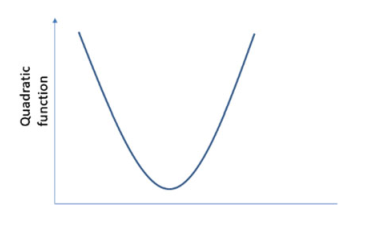
\includegraphics[width=0.55\textwidth]{bilder/quadratic_func.PNG}
	\caption{Visualisierung der allgemeinen Form einer quadratischen Gleichung. Diese entspricht einer Parabel\cite{IntroML}.}
	\label{parabel}
\end{figure}

\newpage
Zunächst hat die Abbildung genau einen Minimum-Wert. Des Weiteren existiert ein lokales Minimum, so dass alle Werte, die außerhalb des Minimums liegen, größer sind. Außerdem sagt das Vorzeichen der Steigung aus, ob der Gradient links oder rechts von dem Minimum liegt. Der Gradient wird auf dieser Kurve zum Minimum hin absteigen, wobei die Steigungsrichtung und der Wert als Orientierungshilfe verwendet werden. Letztendlich nutzt der Gradientenabstieg für die Lösung des Verfahrens genau diese drei genannten Eigenschaften. 





\paragraph{Bestimmung der Steigung}
%%book c

~\newline

Von den Koeffizienten $\theta_0$ bis $\theta_n$ hängt die Kostenfunktion $J(\theta)$ ab. Diese Koeffizienten müssen bestimmt werden. Dieses Verfahren, das das Finden von Gradienten in Bezug auf nur eine Variable realisiert, wird auch als partielle Ableitung bezeichnet und mit dem Symbol $\partial$ gekennzeichnet. Zum Beispiel stellt $\frac{\partial J}{\partial \theta_0}$ die Steigung von $J(\theta)$ in Bezug auf $\theta$ dar.
Die Ableitung von der Kostenfunktion (s. Gleichung \ref{quad_fehler}) hat eine einheitliche Darstellung in allen $\theta_j$ ($j = (0,1,2...,n)$:

\begin{equation}
\label{ableitung_partial}
\frac{\partial J}{\partial \theta_j} = \frac{1}{m}\sum_{i=1}^{m}(h(x^i) - y^i)*x_j^i
\end{equation}

\paragraph{Anpassung/Korrektur}
~\newline



Nach der Initialisierung der $\theta$-Koeffizienten mit zufälligen Zahlen kann die Steigung von der Kostenfunktion $J(\theta)$ bezüglich $\theta_j$ bestimmt werden. Anschließend werden alle Koeffizienten mit dem berechneten Wert aktualisiert:

\begin{equation}
\label{}
\theta_j = \theta_j - \alpha*\frac{\delta J}{\delta\theta_j}
\end{equation}

Dabei entspricht $\alpha$ einer Konstante und dient als Korrekturfaktor. Wenn die berechnete Steigung positiv ist, dann wird der Term $\theta_j$ kleiner. Analog gilt es auch für die negative Steigung, die den Wert $\theta_j$ größer macht. Dies wird solange wiederholt, bis das Minimum der Kostenkurve erreicht wurde. 


\paragraph{Lernrate}
~\newline


Da die Gleichung \ref{ableitung_partial} nur die Steigung berechnet und nur die Richtung angibt, ob $\theta_j$ erhöht oder erniedrigt werden soll, wird ein Mechanismus benötigt, welches der Aktualisierung mitteilt, wie weit in eine bestimmte Richtung aktualisiert werden darf. Ein solcher Mechanismus $\alpha$ wird auch als Lernrate bezeichnet.

\begin{figure}[h!]
	\centering
	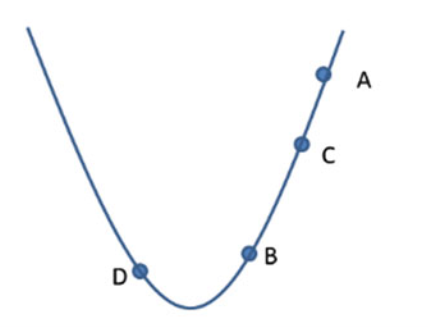
\includegraphics[width=0.65\textwidth]{bilder/quadratic_func_labeled.png}
	\caption{Visualisierung der Kostenfunktion mit vier verschiedenen Punkten, die durch eine bestimme Lernrate erreicht werden kann.\cite{IntroML}.}
	\label{lernrate}
\end{figure}


Die Abbildung \ref{lernrate} zeigt eine Kostenfunktion mit vier verschiedenen Punkten. Ausgehend von der Position A wird die Steigung berechnet. Um das Minimum zu erreichen, muss der Wert $\theta_j$ in die linke Richtung aktualisiert werden. Diese Information ist in der Steigung aufgrund des positiven Wertes gegeben. Eine hohe Lernrate sorgt dafür, dass ein großer Schritt in Richtung des Minimums gemacht wird, so dass der Punkt B erreicht wird. Allerdings kann es bei der nächsten Iteration sein, dass das Minimum übersprungen wurde und $\theta_j$ sich bei dem Punkt D aufhält. Bei einer kleinen Lernrate wird beispielsweise der Punkt C ausgehend von Punkt A erreicht. Die Konsequenz aus einer kleinen Lernrate ist, dass viel öfter iteriert werden muss, um das Minimum zu erreichen. Außerdem dauert die Berechnung dadurch länger. Die Berechnungen werden solange fortgeführt, bis die Lösung des gewünschten Wertes konvergiert.

%%abschnitt konvergenz erstmal rausgelassen

\subsubsection{Fehlerrückführung}


%978

Die Fehlerrückführung (engl. back propagation) berechnet die Gradienten und ordnet dementsprechend die richtigen Eingänge den richtigen Ausgängen zu. Das Verfahren besteht aus zwei Schritten, nämlich die Propagationsphase sowie die Aktualisierung der Gewichte aller Neuronen. Der Pseudocode \ref{pseudo_back} fasst die notwendige Schritte zusammen. Zunächst werden die Gewichte mit zufälligen Werten in der Propagationsphase bereitgestellt. Anschließend werden die Beispiele aus dem Datensatz mit dem Modell klassifiziert und deren Fehler bestimmt. In der Fehlerrückführungsphase werden die Gewichte jeweils von der versteckten Schicht zur Ausgabeschicht sowie von der Eingabeschicht zur versteckten Schicht berechnet, um die aktuelle Gewichte des Netzwerks aktualisieren zu können\cite{Bell2014}.

\begin{lstlisting}[caption={Der Pseudocode zu dem Fehlerrückführung-Algorihtmus beschreibt die notwendigen Schritte\cite{Bell2014}.}, label=pseudo_back]
Initialisierung der Gewichte mit Zufallswerten;
while(Beispiele noch vorhanden):
	Für jedes Beispiel x:
		Vorhersage  = neural_output(network, x)
		aktuell  = korrektes_label(x)
		Fehler ist (Vorhersage - aktuell) an den Ausgabenknoten;
		
Fehlerrückführung:
	- Berechne Gewichte von der versteckten Schicht zur Ausgabeschicht;
	- Berechne Gewichte von der Eingabeschicht zur versteckten Schicht;
	- Aktualisiere Gewichte von dem Netzwerk bis alle korrekt anhand der Trainingsdaten klassifiziert wurden;
	- Rückgabe des abgeschlossenen Netzwerks;
\end{lstlisting}



% book h backpropagation seite 55

%%%%%%%%%%%%%%%%%%%%%%%%%%%%%%%%%%%%%%%%%%%%%%%%%%%%%%%%%%%%%%%%%%%%%%%%%%%%%%%%%%%%%%
% 129 seite 953
%TODO: Zeilenumbrüche, ell und L unterschied

\paragraph{Mathematischer Hintergrund}
~\newline

In diesem Abschnitt wird der Pseudocode aus der Perspektive der Mathematik betrach-\newline tet\cite{Gonzalez2018}.
\newline

Um die Parameter des neuronalen Netzes finden zu können, werden die Trainingsdaten benötigt, um den Fehler zu minimieren. Mittels einer Fehlerfunktion wird der Durchschnitt der Unterschiede zwischen gewünschten und tatsächlichen Antworten gemessen. Die Variable \textbf{r} soll die gewünschte Antwort für einen gegebenen Mustervektor \textbf{x} repräsentieren. Des Weiteren beschreibt \textbf{a}(\texttt{L}) die tatsächliche Antwort des Netzes zu der Eingabe. 


Die Aktivierungswerte von dem Neuron \texttt{j} in der Ausgabeschicht werden als $a_j$(\texttt{L}) bezeichnet. Der Fehler dieses Neurons wird folgendermaßen für $j = 1,2,...,n\texttt(L)$ definiert:

\begin{equation}
\label{fehler_E}
	E_j = \frac{1}{2}(r_j - a_j(L))^2
\end{equation}

Für ein gegebenes Muster $x$ ist $r_j$ die gewünschte Antwort des Ausgangsneurons $a_j$(\texttt{L}). Der Ausgabefehler zu einem einzelnen Muster ist die Summe der Fehler aller Ausgabeneuronen:

\begin{equation}
E = \sum_{j = 1}^{n_L}(r_j -a_j(L))^2 \\\\
 = \frac{1}{2}\Vert{r - a(L)}\Vert^2
\end{equation}

Diese Summe lässt sich auch als euklidische Vektornorm definieren. Der Gesamtfehler aller Trainingsmuster ist als die Summe der Fehler der einzelnen Muster definiert. Das Ziel ist hierbei Gewichte mithilfe des Gradientenabstiegs zu finden, welche diesen Gesamtfehler minimieren. Da wir die Gradienten der Gewichte in den versteckten Knoten nicht berechnen können, wird der Backpropagation-Algorithmus verwendet, welcher den Ausgabefehler in das Netzwerk weiterleiten kann. Um dies zu ermöglichen, muss die Frage beantwortet werden, wie sich der Fehler \texttt{E} bezüglich der Gewichte im Netzwerk ändert. Der Ausdruck $\partial E/\partial z_j(\ell)$ ist die Steuergröße für die Anpassung, wobei $\partial z_j(\ell)$ die Netzeingabe zu dem Knoten $j$ in der $\ell$-Schicht ist. Zur Vereinfachung wird ein neues Symbol $\delta_j(\ell)$ eingeführt, das den Ausdruck $\partial E/\partial \delta_j(\ell)$ repräsentiert. Der Backpropagation-Algorithmus beginnt zunächst mit der Ausgabe: 

\begin{equation}
\label{delta_hidden}
\delta_j(L) = \frac{\partial E}{\partial z_j(L)}
\end{equation}

%\begin{equation}
%12.54 nötig??
%\end{equation}

Mithilfe der Kettenregel kann dieser Ausdruck in Bezug auf die Ausgabe $a_j(L)$ weiter umformuliert werden:

\begin{equation}
\delta_j(L) = \frac{\partial E}{\partial z_j(L)} = \frac{\partial E}{\partial a_j(L)}\frac{\partial a_j(L)}{\partial z_j(L)} = \frac{\partial E}{\partial a_j(L)}\frac{\partial h(z_j(L))}{\partial z_j(L)}
\newline =  \frac{\partial E}{\partial a_j(L)}h'(z_j(L))
\end{equation}

Das Symbol $h$ soll die Aktivierungsfunktion darstellen, die die Netzeingabe $z_j$ in der letzten Schicht $L$ als Parameter hat. Die Ableitung der Aktivierungsfunktion ist aus der Gleichung \ref{ableitung_sig} bekannt. Des Weiteren lässt sich der Fehler (s. Gleichung \ref{fehler_E}) nach $a$ ableiten. Die Gleichung sieht nun folgendermaßen aus:  

\begin{equation}
\delta_j(L) = h(z_j(L))[1 - h(z_j(L))] [a_j(L) - r_j]
\end{equation}

Der Termausdruck $h(z_j(L))]$ ist bekannt, wenn durch alle Neuronen von der ersten bis zu der letzten Schicht im Netzwerk traversiert wurde. Die Aktivierungswerte $a_j(L)$ können in der Ausgabe des Netzwerks beobachtet werden. Außerdem ist die Variable $r_j$ mit dem Muster $x$ während des Trainings ersichtlich und somit kann der Ausdruck $\delta_j(L)$ berechnet werden. 
Da die Beziehung zwischen dem Netzeingang und dem Ausgang eines beliebigen Neurons in einer beliebigen Schicht $\ell$ gleich ist, gilt die Gleichung \ref{delta_hidden} für jeden Knoten $j$ in einer versteckten Schicht:

\begin{equation}
\label{zujedemneuron}
\delta_j(\ell) = \frac{\partial E}{\partial z_j(\ell)}
\end{equation}

Die Gleichung \ref{zujedemneuron} beschreibt, wie sich der Fehler in Bezug auf eine Änderung des Netzeinganges zu jedem Neuron im Netzwerk ändert. Der nächste Schritt ist den Ausdruck $\delta_j(\ell)$ in Form von $\delta_j(\ell + 1)$, umzuformulieren. Da der Fehler im Netzwerk rückwärts zurückgeführt werden soll, ist die Beziehung zwischen den beiden Ausdrücken unabdingbar, um den Ausdruck $\delta_j(L - 1)$ ausgehend von $\delta_j(L)$ zu finden. Das gefundene Ergebnis wird weiter verwendet, bis die zweite Schicht und so weiter erreicht wurde. Mithilfe der Kettenregel kann der gewünschte Ausdruck formuliert werden:

\begin{equation}
\begin{split}
	\delta_j(\ell) = \frac{\partial E}{\partial z_j(\ell)} = \sum_{i}\frac{\partial E}{\partial z_j(\ell + 1)} \frac{\partial z_j(\ell + 1)}{\partial a_j(\ell)}\frac{\partial a_j(\ell)}{\partial z_j(\ell)}  \\
	= \sum_{i}\delta_i(\ell + 1) \frac{\partial z_j(\ell + 1)}{a_j(\ell)}h'(z_j(\ell)) = h'(z_j(\ell))\sum_{i}\omega_{ij}(\ell + 1)\delta_i(\ell + 1)
\end{split}
\end{equation}

In der Gleichung gilt $\ell = L-1, L-2,...,2$. Die aktuelle Antwort des Netzwerks $a_j$ kann durch $h'(z_j(\ell))$ ersetzt werden. Des Weiteren wird die Gleichung \ref{zujedemneuron} angewendet, um zu der letzten Formulierung zu gelangen. Die Gesamteingangsgröße $z_i$ für das Neuron $i$ in der Schicht $\ell$ lässt sich auch als Summe der Gewichte von jeweiligen Kanten mit den Antworten der vorherigen Schicht beschreiben.
Der aktuelle Stand ist, dass der Fehler bei der Ausgabe berechnet werden kann. Des Weiteren steht eine Funktion zur Verfügung, die die Veränderung des Fehlers zu jedem Knoten im Netzwerk beschreiben kann. Der nächste Schritt ist nun, den Ausdruck $\partial E/\partial w_{ij}$ in Bezug auf $\delta_j(\ell)=\partial E/z_j(\ell)$ zu erhalten. Auch hierfür wird die Kettenregel nochmal angewendet:

\begin{equation}
\frac{\partial E}{\partial \omega_{ij}(\ell)} = \frac{\partial E}{\partial z_i(\ell)}\frac{\partial z_i(\ell)}{\partial \omega_{ij}(\ell)} = \delta_i(\ell)\frac{\partial z_i(\ell)}{\partial \omega_{ij}(\ell)} = a_j(\ell - 1)\delta_i(\ell)
\end{equation}

Die Gleichung \ref{zujedemneuron} wurde verwendet, um die Umformung zu vereinfachen. Außerdem entspricht der Ausdruck $\partial z_i(\ell)/\partial \omega_{ij}(\ell)$ dem Term $a_j(\ell - 1)$. 
Da die Änderungsrate von $E$ in Bezug auf die Gewichte berechnet werden kann, ist nun die Aktualisierung der letzte Schritt:


% bias raus erstmal
%\begin{equation}
%\frac{\partial E}{\partial b_i(\ell)} = \delta_i(\ell)
%\end{equation}


\begin{equation}
\omega_{ij}(\ell) = \omega_{ij}(\ell) - \alpha\frac{\partial E(\ell)}{\partial \omega_{ij}(\ell)} = \omega_{ij}(\ell) - \alpha\delta_i(\ell)a_j(\ell - 1)
\end{equation}

Die Lernrate $\alpha$ wird bei dem Vorwärtspass berechnet und bei dem Gradientenabstieg verwendet. Die Berechnungen von $\delta$ werden während des Backpropagation-Algorithmus ermittelt. 



%%bias ignorieren
%\begin{equation}
%b_i(\ell) = b_i(\ell) - \alpha \frac{\partial E}{\partial b_i(\ell)} = b_i(\ell) - \alpha \delta_i(\ell)
%\end{equation}


\section{Convolutional Neural Networks}
%Begriffe poolingschicht ect einheitlich

Die mathematische Faltung ist ein sehr wichtiges Konzept aus dem Bereich des maschinellen Lernens. Mithilfe der Faltung können wichtige Merkmale automatisiert extrahiert werden, die zur Identifizierung der Zielklassen benötigt werden\cite{IntroML}. Der Vorteil liegt darin, dass dieser Ansatz alle räumlichen Beziehungen nutzt, die zwischen Pixeln in einem Bild bestehen können, zum Beispiel Pixelanordnungen in Ecken, das Vorhandensein von Kantensegmenten und anderen Merkmalen, um ein Bild von einem anderen unterscheiden zu können. Daher wird in diesem Abschnitt eine neue Klasse von neuronalen Netzwerken vorgestellt, die als Convolutional Neural Networks (engl. CNN) bezeichnet werden. Außerdem können solche Netze Bilder als Eingabe akzeptieren und eignen sich für das automatische Lernen und die Bildklassifizierung\cite{Gonzalez2018}.

\subsection{Aufbau}

Der allgemeine Aufbau von Faltungsnetzen\cite{Gonzalez2018, IntroML} besteht aus mehreren Schichten von Faltungsschichten zu Poolingschichten, die oft wiederholt werden, um lokale Merkmale aus Eingangsbildern zu lokalisieren und anschließend diese mathematisch zu falten sowie die Dimension des Bildes zu reduzieren. Durch diese Vorgehensweise können Merkmale gefunden werden, die in sehr abstrakter Form vorliegen. Nach einer bestimmten Anzahl von Wiederholungen der Schichten folgt ein klassisches neuronales Netz, welches die Klassifikation durchführt. Die generelle Funktionsweise von Faltungsschichten und Poolingschichten werden in den Abschnitten \ref{sec:faltungsschicht} und \ref{sec:poolingschicht} erläutert. 

Die Abbildung \ref{cnn_arch} visualisiert den klassischen Aufbau eines Faltungsnetzes. Das Faltungsnetz nimmt ein Bild als Eingabe an. Mithilfe der Faltungsschicht wird die Eingabe abgetastet und mathematisch gefaltet. Dadurch entstehen mehrere Feature-Maps, dessen Dimensionen in anschließendem Schritt reduziert wird. Dann folgt wieder eine Faltungsschicht, die die Anzahl der Feature-Maps erhöht. Daraufhin wird ein letztes Mal eine Poolingschicht angewendet. Anschließend kann ein klassisches neuronales Netz Feature-Maps als Vektor annehmen, um eine Klassifikation durchführen zu können\cite{Gonzalez2018}.

\begin{figure}[h!]
	\centering
	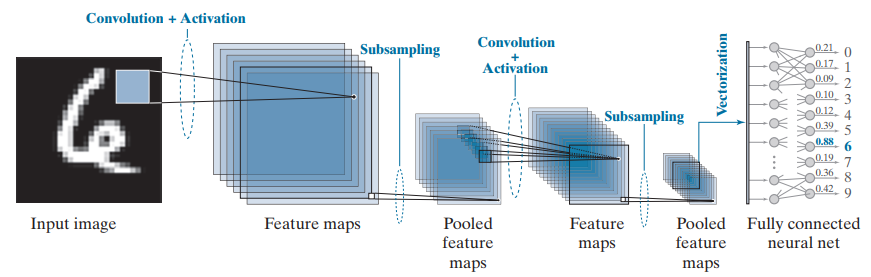
\includegraphics[width=\textwidth]{bilder/cnn_arch.PNG}
	\caption{Darstellung der verschiedenen Funktionen eines CNNs. Dabei wird das Eingangsbild am Ende als die Zahl sechs klassifiziert. Hierfür werden die Feature-Maps vektorisiert, um eine Klassifikation zu ermöglichen\cite{Gonzalez2018}.}
	\label{cnn_arch}
\end{figure}

\subsection{Faltungsschicht}
\label{sec:faltungsschicht}
% anderer Titel


Der grundlegende Unterschied zwischen einer klassischen verbundenen Schicht bei einem neuronalen Netz und einer Faltungsschicht (engl. convolution layer) besteht darin, dass die typische Schicht globale Muster versucht zu lernen. Die Faltungsschicht lernt stattdessen lokale Muster, die aus kleinen 2D-Fenstern bestehen. Die Abbildung \ref{convolution_example} zeigt eine handgeschriebene vier, aus der drei lokale Muster in der Größe von 3 x 3 erkannt wurden\cite{francois}.

\begin{figure}[h!]
	\centering
	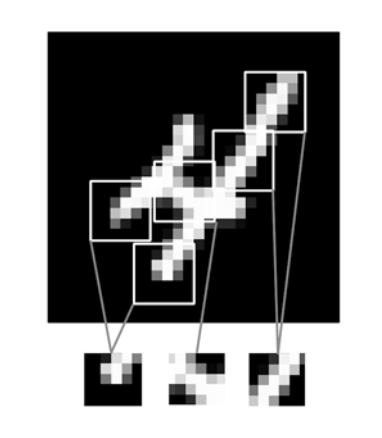
\includegraphics[width=0.7\textwidth]{bilder/convolution_example.PNG}
	\caption{Bilder können in lokale Muster wie Kanten oder Texturen unterteilt werden. Hier wurden drei Muster in dem Bild erkannt\cite{francois}.}
	\label{convolution_example}
\end{figure}

\newpage
~\newline
Grundsätzlich haben CNNs zwei wichtige Eigenschaften\cite{francois}:

\begin{itemize}
	\item \textbf{Translationsinvariante}: Mithilfe dieser Eigenschaft können CNNs nach dem Erlernen eines bestimmten Musters, ortsunabhängig in dem ganzen Bild das Muster wiedererkennen. Bei den klassischen neuronalen Netzen müsste das Muster neu gelernt werden, wenn die Position des Musters aus den Trainingsdaten abweicht. 
	Ein weiterer Vorteil ist, dass weniger Trainingsproben benötigt werden, um Darstellungen zu erlernen, die für die Generalisierung hilfreich sind.
	
	\item \textbf{Räumliche Musterhierarchien}: Da CNNs aus mehreren Faltungsschichten bestehen, lernt die erste Faltungsschicht kleine lokale Muster wie Kanten. Die nächste Schicht lernt größere Muster aus den Merkmalen der ersten beziehungsweise vorherigen Schichten. Dadurch können CNNs immer komplexere und abstraktere visuelle Darstellungen effizient erlernen. Dabei bildet sich eine Hierarchie aus Mustern. Die Abbildung \ref{cat_pattern} zeigt eine solche Hierarchie. Bestehend aus einfachen unterschiedlich aussehenden Kanten werden Konstrukte, zum Beispiel die Nase, Augen und Ohren, gebildet, um eine Katze klassifizieren zu können.
	

	\begin{figure}[h!]
		\centering
		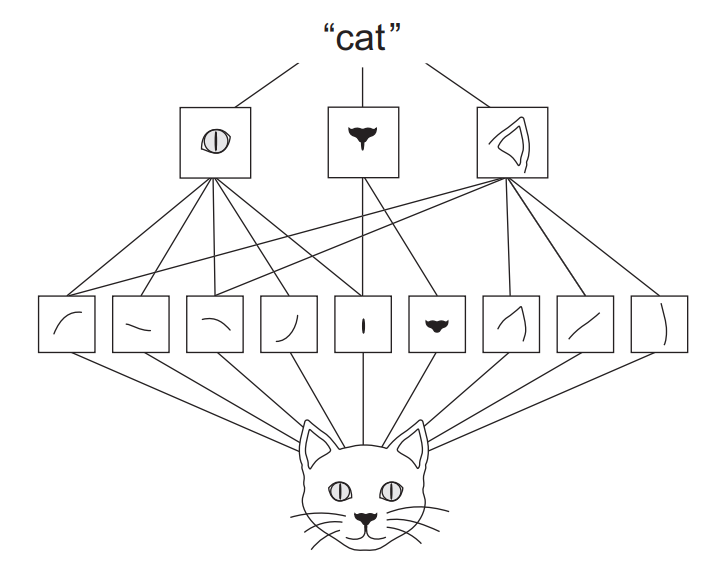
\includegraphics[width=0.7\textwidth]{bilder/cat_pattern.PNG}
		\caption{Lokale Kanten verbinden sich zu lokalen Objekten wie Augen oder Ohren, um die Klasse \glqq Katze\grqq~erkennen zu können\cite{francois}.}
		\label{cat_pattern}
	\end{figure}
	
\end{itemize}



Neben der zwei wichtigsten Eigenschaften arbeiten Faltungsschichten auf einer so genannten Feature-Map mit zwei räumlichen Achsen, hier Höhe und Breite, sowie eine Tiefenachse. Zum Beispiel ist die Dimension der Tiefenachse bei einem RGB-Bild drei, da das Bild drei Farbkanäle beinhaltet, nämlich rot, grün und blau. Die Faltungsoperation extrahiert Felder aus ihrer Input-Feature-Map und wendet die gleiche Transformation auf alle diese Felder an, wodurch eine Output-Feature-Map entsteht. Diese Feature-Map ist immer noch ein 3D-Würfel. Allerdings kann die Tiefe beliebig sein, da die Ausgabetiefe ein Parameter der Ebene ist und die verschiedenen Kanäle in dieser Tiefenachse nicht mehr für bestimmte Farben wie beim RGB-Eingang stehen, sondern für die Anzahl der Filter. Ein Filter kodiert bestimmte Aspekte der Eingangsdaten\cite{francois}. 

Die Funktionsweise einer Faltung lässt sich folgendermaßen erläutern\cite{francois}. Zunächst wird ein Fenster der Größe 3 x 3 oder 5 x 5 über die dreidimensionale Feature-Map verschoben, um ein dreidimensionales Teilstück zu extrahieren. Diese Operation wird an jeder möglichen Stelle ausgeführt. Jedes dreidimensionale Teilstück wird dann in einen eindimensionalen Formvektor transformiert. Alle diese Vektoren werden dann räumlich zu einer dreidimensionalen Feature-Map mit den Dimensionen, also Höhe, Breite und Ausgabetiefe, zusammengefügt. Die Abbildung \ref{feature_map_extraction} visualisiert die beschriebene Schritte.

\begin{figure}[h!]
	\centering
	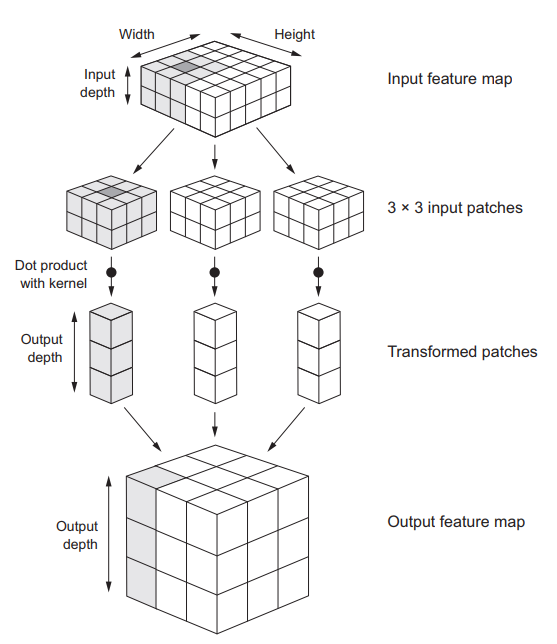
\includegraphics[width=0.7\textwidth]{bilder/feature_map_extraction.PNG}
	\caption{Visualisierung der Zusammensetzung von neuen Feature-Maps mittels der mathematischen Faltung\cite{francois}.}
	\label{feature_map_extraction}
\end{figure}
%% über padding schreiben


\subsection{Poolingschicht}
\label{sec:poolingschicht}
%book i

Die Poolingschicht ist eine Möglichkeit der Nachverarbeitung, wie die Daten in den Feature-Maps nach verarbeitet werden können\cite{francois}. Ein Fenster, das die Größe 2 x 2 hat, durchläuft die Feature-Map und extrahiert Werte. Abhängig von der Operation, zum Beispiel das Maximum, das Minimum oder der Durchschnitt, werden alle umliegenden Werte betrachtet. Ein einzelner Wert repräsentiert die umliegenden Pixel in dem Fensterausschnitt\cite{IntroML}. Ein großer Unterschied zu der Faltungsschicht besteht darin, dass Feature-Maps um den Faktor zwei verkleinert werden, um die Koeffizienten in den Feature-Maps zu reduzieren\cite{francois}. Des Weiteren glättet ein solches Verfahren Feature-Maps. Bei einer Max-Poolingschicht wird ein sehr hoher Wert in die umgebenden Werte einfließen, so dass die genaue Position in der Feature-Map nicht mehr relevant ist. Vielmehr wird nun auf den allgemeinen Bereich, also an und um diese Position herum, fokussiert \cite{IntroML}.


Die Abbildung \ref{cnn_pooling_example} zeigt die Dimensionreduktion nach der Poolingschicht. Das Eingabebild ist zunächst 28 x 28 groß. Nach der mathematischen Faltung in der Faltungsschicht ist die Feature-Map auf 24 x 24 verkleinert. In dieser Feature-Map werden vier benachbarte Werte innerhalb des 2 x 2 großen Fensters anschließend zu einem Wert zusammengeführt, so dass die Größe nun bei 12 x 12 liegt. Außerdem entspricht die Reduzierung der Dimension dem Faktor zwei.


\begin{figure}[h!]
	\centering
	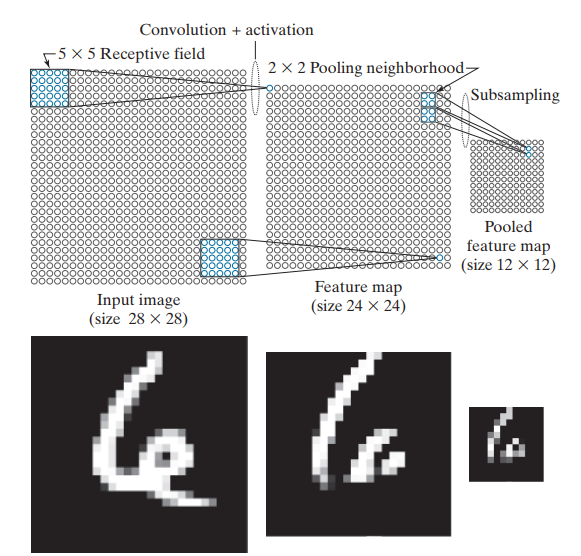
\includegraphics[width=0.75\textwidth]{bilder/convolution_example2.PNG}
	\caption{Veranschaulichung der Konsequenz nach der Poolingschicht. Die Ausgangsgröße der Feature-Map (24 x 24) verkleinert sich auf eine Größe von 12 x 12\cite{Gonzalez2018}.}
	\label{cnn_pooling_example}
\end{figure}



\subsection{Regularisierung}
%TODO: Bessere Abgrenzung von paragraph

%book b 139

Der Begriff Regularisierung beschreibt einen Prozess, welcher die Überanpassung eines Modells reduzieren kann. Es ist eine Möglichkeit, den Lernprozess zu warnen, dass bestimmte Daten ein Rauschen vorweisen oder das Modell auswendig gelernt haben können\cite{Nelli2018}. 


\subsubsection{Gewichtsregulierung}
%book b 139
Falls Daten ein gewisses Rauschen vorweisen, ist es dank der Gewichtsregulierung möglich, die Modellgewichte im Falle einer Überpassung zu bestrafen\cite{Nelli2018,Vasilev2019}. Bei dem Lernverfahren werden die Gewichte der Neuronenverbindungen nach jeder Iteration aktualisiert. Beim Auftreten einer verrauschten Probe kann das Modell fälschlicherweise annehmen, dass diese Probe gültig ist und versucht das Muster, anzupassen\cite{Nelli2018,Subramanian2018}. Durch die Anpassung werden die Gewichte dementsprechend geändert und die Veränderung kann enorm sein. Normalerweise weisen verrauschte Proben keine Ähnlichkeit mit normalen Datenpunkten auf, da sie weit entfernt von ihnen sind. Die Lösung des Problems ist, dass die Gewichte der Kanten zur definierten Verlustfunktion dazu addiert werden und somit ganzheitlich höhere Kosten darstellen. Dann kann das Modell sich selbst abstimmen, um den Verlust zu reduzieren und sorgt dafür, dass die Aktualisierung der Gewichte in die richtige Richtung geht. Die allgemeine Regularisierung lässt sich folgendermaßen beschreiben:

\begin{equation}
Kosten = Verlust + Hyperparameter~x~[Gewichte]
\end{equation}

Dabei entspricht der Hyperparameter dem Ausdruck $\frac{\lambda}{2m}$ und der Wert $\lambda$ wird von dem Anwender definiert. Da einige Regularisierungen existieren, werden hier nur zwei vorgestellt, nämlich L1 und L2.


\paragraph{L1-Regularisierung}
~\newline


Die absoluten Gewichte werden bei der L1-Regularisierung zur Verlustfunktion addiert. Für die Generalisierung des Modells werden die Werte der Gewichte auf null reduziert. Des Weiteren sorgt dieses Verfahren für eine schnellere Berechnung\cite{Nelli2018}.
\newline
Die L1-Regularisierung lässt sich folgendermaßen beschreiben:

\begin{equation}
	Kosten = Verlust + \frac{\lambda}{2m}*\sum\vert\vert Gewichte\vert\vert
\end{equation}



\paragraph{L2-Regularisierung}
~\newline

Bei diesem Verfahren werden die Gewichte quadriert zur Verlustfunktion hinzugefügt. Im Gegensatz zu dem L1-Verfahren werden die Werte der Gewichte auf bei nahezu null reduziert. In den meisten Fällen wird die L2-Regularisierung gegenüber der L1-Regularisierung bevorzugt, um die Überpassung zu reduzieren\cite{Nelli2018}.
\newline
Die mathematische Formulierung kennzeichnet sich durch diese Gleichung:

\begin{equation}
Kosten = Verlust + \frac{\lambda}{2m}*\sum\vert\vert Gewichte\vert\vert^2
\end{equation}

%%erstmal raus
%%\subsubsection{Early-Stopping}
\subsubsection{Dropout-Verfahren}

Für neuronale Netze ist das Dropout-Verfahren eine der effektivsten und am häufigsten verwendeten Regularisierungstechniken. Die Idee hinter diesem Verfahren liegt darin, während des Lernens die Ausgabefunktion in einer Schicht zufällig auf null zu setzen\cite{francois}. Dadurch ändert sich die Struktur des Modells, so dass Variationen an Parametersätzen entstehen\cite{Gonzalez2018}. Des Weiteren gibt die Dropout-Rate an, wie hoch der Anteil der Datenpunkte auf den Wert null gesetzt werden sollen. In der Regel liegt der Anteil zwischen 0.2 und 0.5\cite{francois, Moolayil2018}.

In Abbildung \ref{dropout} werden einige Knoten in dem neuronalen Netz in jeder Schicht nicht mehr angesprochen.

\begin{figure}[h!]
	\centering
	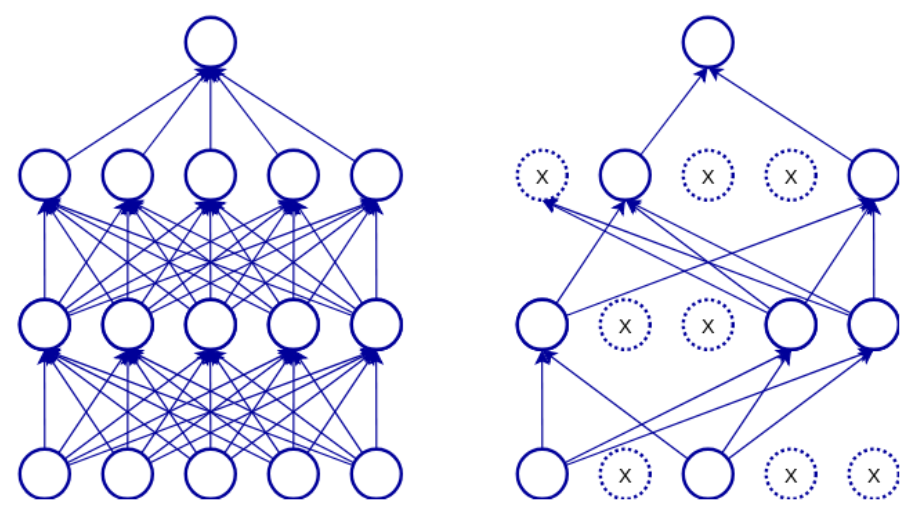
\includegraphics[width=1\textwidth]{bilder/dropout.PNG}
	\caption{In der linken Darstellung wird ein komplett vernetztes Netzwerk angezeigt. Ausgehend von dieser Struktur können einige Knoten in jeder Schicht (rechts) ausgeschlossen werden\cite{Vasilev2019}.}
	\label{dropout}
\end{figure}

\section{Bibliotheken}
%TODO: Tensorflow und GPU Computing/Parallel Computing, book d
%%book h
Zahlreiche Open-Source-Bibliotheken erlauben die Implementierung von tiefen neuronalen Netzen in der Programmiersprache Python. Dabei wird der Code nicht von Grund auf neu geschrieben, weil diese Bibliotheken auf die Grundeinheit für die Datenspeicherung (Tensor) nutzen. Ein Tensor ist eine Verallgemeinerung einer Matrix in höheren Dimensionen bestehend aus mehrdimensionalen Arrays von Basiswerten, die typischerweise von 16 bis 64-Bit Float beziehungsweise Integer repräsentieren. In diesem Abschnitt werden folgende Bibliotheken vorgestellt: Keras und Pytorch\cite{Vasilev2019}.


\subsection{Keras}
%%book i
\label{sec:keras}
Die Bibliothek Keras ermöglicht eine komfortable Definition und Umsetzung von neuronalen Netzen jeglicher Art\cite{francois}. Ursprünglich wurde diese Bibliothek für Forscher entwickelt, um schnelle Experimente zu ermöglichen. Daher verfügt diese Bibliothek über eine integrierte Unterstützung für Faltungsnetzwerke, wiederkehrende Netzwerke (engl. recurrent network) und jede Kombination von beidem. Des Weiteren werden beliebige Netzwerkarchitekturen unterstützt, zum Beispiel Modelle mit mehreren Eingängen
beziehungsweise Ausgängen.

\begin{figure}[h!]
	\centering
	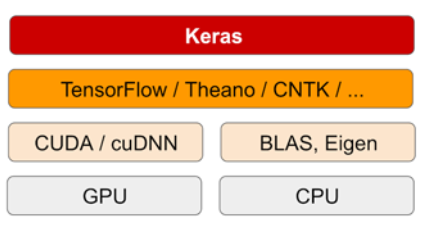
\includegraphics[width=0.7\textwidth]{bilder/keras_backend.PNG}
	\caption{In dieser Grafik wird die Flexibilität von Keras bezüglich des Backends sowie der Prozessoreinheit visualisiert\cite{francois}.}
	\label{keras_backend}
\end{figure}

Da die Bibliothek Keras nicht als Backend fungiert, wird Keras folgende Backends unterstützt: TensorFlow, CNTK und Theano. Jeder Programmiercode, welcher mit Keras geschrieben wurde, kann mit jedem dieser Backends ausgetauscht sowie ausgeführt werden. Hierbei werden keine Anpassungen des Codes benötigt (s. Abbildung \ref{keras_backend})\cite{francois}.  

\subsubsection{Erstellung des Modells}

Die Keras Bibliothek bietet zwei Möglichkeiten, wie ein Modell definiert werden kann. Mit der \textbf{Sequential}-Klasse können linear aufgebaute Modelle, die der häufigsten Netzwerkarchitektur entsprechen, erstellt werden. Mit der \textbf{Functional}-API können beliebige Architekturen gebaut werden, wenn die Struktur der Schichten einem direkten azyklischen Graphen ähnelt. Der Aufbau der zwei Möglichkeiten ist ähnlich. Zunächst müssen Eingabe-Tensoren und Ziel-Tensoren definiert werden. Anschließend wird ein Netzwerk mit Schichten erstellt, welches die Eingaben auf die Ziele abbildet\cite{francois}.

Der Code-Abschnitt \ref{model_seq} zeigt, wie ein Modell mit der \textbf{Sequential}-Klasse erstellt wird. In der ersten Schicht wird die erwartete Form der Eingangsdaten übermittelt.

\begin{lstlisting}[caption={Erstellung eines Modells mit der \textbf{Sequential}-Klasse\cite{francois}.}, label=model_seq]
from keras import models
from keras import layers
model = models.Sequential()
model.add(layers.Dense(32, activation='relu', input_shape=(784,)))
model.add(layers.Dense(10, activation='softmax'))
\end{lstlisting}

Mit der \textbf{Functional}-API werden die Tensoren manipuliert, die vom Modell verarbeitet werden, um diese auf Schichten anzuwenden. Daher werden Tensoren als Funktionsparameter übergeben (s. Code \ref{model_functional}).

\begin{lstlisting}[caption={Ein anderer Ansatz zu der Erstellung eines Modells mittels der \textbf{Functional}-API\cite{francois}.}, label=model_functional]
input_tensor = layers.Input(shape=(784,))
x = layers.Dense(32, activation='relu')(input_tensor)
output_tensor = layers.Dense(10, activation='softmax')(x)
model = models.Model(inputs=input_tensor, outputs=output_tensor)
\end{lstlisting}

\subsubsection{Das Kompilieren eines Modells}
Nach der Erstellung des Modells ist der nächste Schritt die Konfiguration des Trainings\cite{francois}. Diese Konfiguration findet im Kompilierungsschritt statt, in dem die Optimierungs- und Verlustfunktionen angeben werden. Des Weiteren können Metriken benutzt werden, um während des Trainings das Lernen des Modells zu überwachen. Der Code \ref{kcc} zeigt ein Beispiel mit dem RMSprop-Gradientenverfahren sowie der mittleren quadratischen Abweichung als Verlustfunktion. In der Dokumentation von Keras können weitere Optimierungs- und Verlustfunktionen gefunden werden\cite{keras_doc}.


\begin{lstlisting}[caption={Die Kompilierung eines Modells\cite{francois}.}, label=kcc]
from keras import optimizers
model.compile(optimizer=optimizers.RMSprop(lr=0.001),
	loss='mse',
	metrics=['accuracy'])
\end{lstlisting}


\subsubsection{Das Trainieren des Modells}
Um das Training zu starten, werden über die \textit{fit()}-Methode die Eingabedaten und dementsprechend Zieldaten übergeben. Des Weiteren benötigt diese Methode die Anzahl der Epochen sowie die Batchgröße. Als Rückgabe wird ein \textit{History-Objekt} zurückgegeben, welches eine Aufzeichnung der Trainingsverlustwerte und Metrikenwerte in aufeinanderfolgenden Epochen sowie der Validierungsverlustwerte und Validierungsmetrikenwerte enthält\cite{francois}.
Der Code \ref{tkc} zeigt den Aufruf der \textit{fit()}-Methode mit der Batchgröße 128 sowie zehn Epochen. Des Weiteren gibt es weitere Abwandlungen der \textit{fit()}-Methode, die in der Quelle zu finden sind\cite{keras_doc}.


\begin{lstlisting}[caption={Das Starten des Trainings mit der \textit{fit()}-Methode\cite{francois}.}, label=tkc]
model.fit(input_tensor, target_tensor, batch_size=128, epochs=10)
\end{lstlisting}


\subsubsection{Einlesen der Daten}
%%book h
Da Dateien im Bildformat vorliegen können, bietet Keras einen Generator, hier ImageDataGenerator, für das Einlesen an. Mit diesem Generator können die eingelesenen Bilder direkt zufällig manipuliert werden\cite{Vasilev2019}. Der Codeabschnitt \ref{idgc} zeigt wie ein ImageDataGenerator-Objekt mit Breiten- und Höhenverschiebung, horizontalem Spiegeln und einigen Normalisierungen erstellt werden kann. 


\begin{lstlisting}[caption={Vorverarbeitung der Bilder mit der \textbf{ImageDataGenerator}-Klasse\cite{Vasilev2019}.}, label=idgc]
data_generator = ImageDataGenerator(rotation_range=90,
width_shift_range=0.1,
height_shift_range=0.1,
featurewise_center=True,
featurewise_std_normalization=True,
horizontal_flip=True)
data_generator.fit(X_train)
\end{lstlisting}

Weitere Operatoren sind in der Quelle\cite{keras_doc} dokumentiert.

\subsubsection{Callbacks}

Mithilfe von Callbacks kann die Kontrolle während des Trainings sowie das Verständnis, was in dem Modell vor sich geht, erlangt werden. Dadurch können schlechte Ergebnisse vermieden werden, wenn die Callbacks-Funktionen Daten an den Bediener zurücksenden und automatisch Steuerungsentscheidungen auf der Grundlage des aktuellen Zustands treffen. Ein Callback ist ein Objekt, das im Aufruf der \textit{fit()}-Methode an das Modell übergeben wird. Letztendlich wird dieses Objekt von dem Modell an verschiedenen Stellen im Training aufgerufen. Das Callback-Objekt hat Zugriff auf alle verfügbaren Daten über den Zustand des Modells und seine Leistung, so dass es Maßnahmen ergreifen kann. Zwei solcher Maßnahmen werden hier kurz vorgestellt\cite{francois}:

\paragraph{EarlyStopping}
~\newline

Mithilfe des \textit{EarlyStopping}-Callback kann das Training unterbrochen werden, wenn eine zu überwachende Zielgröße für eine bestimmte Anzahl von Epochen keine Verbesserung aufweist. Dadurch kann die Überanpassung des Modells mit steigender Epochenanzahl verhindert werden, wenn das Training rechtzeitig nach der definierten Zielgröße abbricht. Der Code \ref{kces} zeigt die Erstellung eines \textit{EarlyStopping}-Callbacks. Callbacks werden als Parameter in der \textit{fit()}-Methode an das Modell übergeben. Das Modell nimmt eine Liste von Callbacks an. In diesem Beispiel wird die Validierungsgenauigkeit des Modells überwacht. Das Training wird unterbrochen, wenn die Genauigkeit seit mehr als einer Epoche nicht mehr verbessert wird.

\begin{lstlisting}[caption={Das frühe Stoppen des Trainings wird mit dem EarlyStopping-Callback veranlasst\cite{francois}.}, label=kces]
callbacks_list = [
	keras.callbacks.EarlyStopping(
		monitor='acc',
		patience=1,
)]

model.fit(x, y,
	epochs=10,
	batch_size=32,
	callbacks=callbacks_list,
	validation_data=(x_val, y_val))
\end{lstlisting}



\paragraph{ModelCheckpoint}
~\newline

Das \textit{ModelCheckpoint}-Callback wird häufig zusammen mit dem \textit{EarlyStopping}-Callback kombiniert, so dass das Modell während des Trainings kontinuierlich gespeichert werden kann. Des Weiteren besteht die Möglichkeit nur das aktuell beste Modell zu speichern. Der Codeabschnitt \ref{kcmc} veranschaulicht, wie das \textit{ModelCheckpoint}-Callback erstellt wird. Zunächst muss der Pfad des zu speichernden Modells definiert werden. Anschließend wird festgelegt, welche Zielgröße überwacht werden soll. Falls der Parameter \glqq save\_best\_only\grqq~auf wahr gesetzt ist, dann wird das zu speichernde Modell nur überschrieben, wenn sich die Zielgröße verbessert hat. Ansonsten werden die Gewichte des Modells bei jeder Epoche abgespeichert.

\begin{lstlisting}[caption={Mithilfe des ModelCheckpoint-Callbacks wird das beste Modell in dem Training abgespeichert\cite{francois}.}, label=kcmc]
keras.callbacks.ModelCheckpoint(
	filepath='my_model.h5',
	monitor='val_loss',
	save_best_only=True)
\end{lstlisting}



\subsubsection{GPU-Support}
Keras ist in der Lage über TensorFlow oder über andere Backends, den Code sowohl auf CPUs als auch auf GPUs auszuführen. Falls das TensorFlow Backend auf der CPU ausgeführt wird, wird eine Low-Level-Bibliothek für Tensoroperationen namens Eigen verwendet. Falls die Ausführung des Codes über eine Grafikkarte verläuft, dann wird eine Bibliothek verwendet, die für Grafikkarten, zum Beispiel NVIDIA CUDA Deep Neural Network Library (cuDNN), optimiert wurde\cite{francois}. 

\subsection{PyTorch}
\label{sec:pytorch}
Dieser Abschnitt basiert auf dem Buch von Vishnu Subramanian\cite{Subramanian2018}.
 
Für die Erstellung von tiefen Faltungsnetzen kennzeichnet sich PyTorch durch die Benutzerfreundlichkeit und Einfachheit. Viele andere gängige Frameworks, die die Erstellung der Faltungsnetze ermöglichen, verwenden statische Berechnungsgraphen. Die Bibliothek PyTorch verfolgt einen anderen Ansatz und bietet einen dynamischen Berechnungsgraphen an, welcher eine größere Möglichkeit bei der Erstellung von komplexen Architekturen anbietet. Ein weiterer Vorteil von PyTorch ist die Verwendung von Python-Konzepten, zum Beispiel Klassen, Strukturen und bedingte Schleifen, um objektorientiert Faltungsnetze aufbauen zu können. Da PyTorch hauptsächlich für die Forschung entwickelt wurde, wird es in bestimmten Szenarien mit sehr geringen Latenzen nicht für den produktiven Einsatz empfohlen.

\subsubsection{Erstellung des Modells}

Alle neuronale Netze werden in PyTorch als Klassen definiert. Des Weiteren wird diese Klasse von \textbf{nn.Module} vererbt. Grundsätzlich sollte ein Konstruktor erstellt werden, um die Initialisierung der Schichten für das Netzwerk zu realisieren. In der PyTorch Dokumentation sind verschiedene Arten von Schichten aufgelistet\cite{pytorch_doc}. In der \textit{forward()}-Methode werden die Eingabedaten an die Schichten übergeben, die im Konstruktor initialisiert wurden. Anschließend wird die Ausgabe zurückgegeben.

Der folgende Codeausschnitt \ref{pytorch_erstellung} zeigt, wie ein tiefes, neuronales Netz in PyTorch implementiert werden kann.

\begin{lstlisting}[caption={Veranschaulichung der typischen Klassenstruktur eines neuronalen Netzes\cite{Subramanian2018}.}, label=pytorch_erstellung]
class MyFirstNetwork(nn.Module):
	def __init__(self, input_size, hidden_size, output_size):
		super(MyFirstNetwork, self).__init__()
		self.layer1 = nn.Linear(input_size, hidden_size)
		self.layer2 = nn.Linear(hidden_size, output_size)
		
	def __forward__(self, input):
		out = self.layer1(input)
		out = nn.ReLU(out)
		out = self.layer2(out)
		return out
\end{lstlisting}

\subsubsection{Das Trainieren des Modells}

Um das Training zu starten, müssen zunächst die Hyperparameter definiert werden. In dem Code \ref{tpt} wird die Lernrate auf 0.001 gesetzt. Die Verlustfunktion ist in diesem Modell die Kreuzentropie und das Lernverfahren wird mit dem stochastischen Gradientenverfahren (engl. SGD) durchgeführt. Die \textit{StepLR()}-Funktion passt die Lernrate während des Trainings dynamisch an.  

\begin{lstlisting}[caption={Definition der Hyperparameter, die in der Training-Methode benötigt werden\cite{Subramanian2018}.}, label=tpt]
learning_rate = 0.001
criterion = nn.CrossEntropyLoss()
optimizer_ft = optim.SGD(model_ft.parameter(),lr=0.001, momentum=0.9)
exp_lr_scheduler.StepLR(optimizer_ft, step_size=7,gamma=0.1)
\end{lstlisting}

Die Methode \textit{$train\_Model$} in dem Code \ref{headh_train} nimmt ein Modell mit den Hyperparametern an und wird für 25 Epochen trainiert. Die Methode selbst lässt sich in vier Abschnitten einteilen. Zunächst erhält das Modell die Bilddateien und berechnet daraus den Verlust.

\begin{lstlisting}[caption={Berechnung der Verluste in der Training-Methode\cite{Subramanian2018}.}, label=headh_train]
def train_model(model, criterion, optimizer, scheduler, num_epochs=25):
	best_model_wts = model.state_dict()
	best_acc = 0.0
	
	for epoch in range(num_epochs):
		for phase in ['train', 'valid']:
			if phase == 'train':
				scheduler.step()
				model.train(True)
			else:
				model.train(False)
				
			running_loss = 0.0
			running_corrects = 0
			
			for data in dataloaders[phase]:
				inputs, labels = data
				inputs, labels = Variable(inputs), Variable(labels)
				
				#zero the parameter gradients
				optimizer.zero_grad()
				
				#forward
				outputs = model(inputs)
				_, preds = torch.max(outputs.data, 1)
				loss = criterion(outputs, labels)
\end{lstlisting}
Während der Trainingsphase wird der Verlust rückwärts propagiert. In der Validierungs- und Testphase werden die Gewichte nicht aktualisert (s. Code \ref{bwppt}).

\begin{lstlisting}[caption={Aktualisierung der Gewichte in der Training-Methode\cite{Subramanian2018}.}, label=bwppt]		
				#backwards
				if phase == 'train':
					loss.backward()
					optimizer.step()
\end{lstlisting}
Im Codeabschnitt \ref{cumulation} wird der Verlust in Batches für jede Epoche kumuliert.

\begin{lstlisting}[caption={Berechnung der Verluste in Batches in der Training-Methode\cite{Subramanian2018}.}, label=cumulation]					
				#statistics
				running_loss += loss.data[0]
				running_corrects += torch.sum(preds == labels.data)
			
			epoch_loss = running_loss / dataset_sizes[phase]
			epoch_acc = running_corrects / dataset_sizes[phase]
			
\end{lstlisting}
			
Der letzte Schritt ist nun das Speichern der Gewichte von dem besten Modell (s. Code \ref{pytorch_save}).
\begin{lstlisting}[caption={Festlegung des besten Modells in der Training-Methode\cite{Subramanian2018}.}, label=pytorch_save]						
			#copy the model
			if phase == 'valid' and epoch_acc > best_acc:
				best_acc = epoch_acc
				best_model_wts = model.state_dict()
	
	#load best model weights
	model.load_state_dict(best_model_wts)
	return model
\end{lstlisting}

\subsubsection{Einlesen der Daten}

Das \textbf{torchvision.datasets}-Paket wird von PyTorch bereitgestellt und wird mittels der Klasse \textbf{ImageFolder} verwendet, um das Laden von Bildern mit den dazugehörigen Labels zu ermöglichen. Nach erfolgreichem Laden der Bilder können Vorverarbeitungsschritte ausgeführt werden. Zum Beispiel können alle Bilder auf eine Größe skaliert werden. Typischerweise wird der Datensatz mit dem Mittelwert und der Standardabweichung des Datensatzes normalisiert. Nach den Vorverarbeitungsschritten können die Daten zu einem PyTorch-Tensor konvertiert werden. 

\begin{lstlisting}[caption={Das Einlesen der Bilddateien wird mit der Klasse \textit{ImageFolder} realisiert\cite{Subramanian2018}.}, label=eddpt]
simple_transform=transforms.compose([transforms.Scale((244,244)),
							transforms.ToTensor(),
							transforms.Normalize([0.485, 0.456, 0.406],
												[0.229, 0.224, 0.225])])
train = ImageFolder('dogsandcats/train/', simple_transform)
valid = ImageFolder('dogsandcats/valid/', simple_transform)
\end{lstlisting}

Der Codeabschnitt \ref{eddpt} zeigt, wie die Bilder mit der Klasse ImageFolder geladen und anschließend diese mit einer einfachen Transformation verändert werden. Hierbei werden die Bilder auf die Größe 244 x 244 skaliert. Anschließend werden die Bilddateien als Tensor konvertiert und mit dem Mittelwert und der Standardabweichung normalisiert. Nach der Erstellung des Objekts für die Transformation wird dieses Objekt als Parameter an die \textbf{ImageFolder}-Klasse übergeben.

\subsubsection{GPU-Support}

Vortrainierte Modelle können auf der Grafikkarte ausgeführt werden. Hierfür muss das Modell die Methode \textit{cuda()} aufgerufen werden. Der Code \ref{gpupt} zeigt diesen Aufruf. 

\begin{lstlisting}[caption={Mit der \textit{cuda()}-Methode wird das Modell auf der Grafikkarte trainiert\cite{Subramanian2018}.}, label=gpupt]
if is_cuda:
	model = model.cuda()
\end{lstlisting}

Für selbst erstellte Modelle muss zunächst das Objekt erlangt werden, welches den Zugriff auf die Grafikkarte hat. Anschließend werden das neuronale Netz und die Daten, also Datenpunkte sowie die Labels, auf die Grafikkarte transferiert (s. Code \ref{transformiert}). 


\begin{lstlisting}[caption={Die Daten und das Modell werden auf die Grafikkarte übertragen, um dort ausgeführt werden zu können\cite{Subramanian2018}.}, label=transformiert]
device = torch.device("cuda:0" if torch.cuda.is_available())

net.to(device)

inputs, labels = data[0].to(device), data[1].to(device)
\end{lstlisting} 


\chapter{Entwurf}
\label{chapter:entwurf}

In diesem Kapitel werden die Anforderungen der Modelle erläutert und die Herangehensweise im Konzept beschrieben.

\section{Anforderungen}

%Anforderungsanalyse 

% Funktionale: 
% blatt nicht erkennen, sondern direkt die Krankheit, Visualisieren
%- Blattkrankheiten, hier benennen 
%- Erkennung von 4 Krankheiten und gesunde blätter
%-- zwei verschiedene Ansätze: Custom Modell, Transfer LEarning
%- speziell ein Voter entwerfen -> für blights
%-- ähnlich symptome aber sehr schwierig zu unterscheiden sind
%- Visualisierung der Schichten


In dieser Masterarbeit soll das zu erstellende Modell, welches mithilfe von Faltungsnetzen realisiert werden soll, die Erkennung der vier Krankheiten sowie gesunden Blättern von einem vorgegebenen Datensatz ermöglichen. Die Krankheiten, hier Dürrfleckenkrankheit, Tomato Yellow Leaf Curl Virus, Samtfleckenkrankheit und Krautfäule, unterscheiden sich ausgehend in der Ausprägung der Symptome stark. Die zwei Krankheiten, Krautfäule und Dürrfleckenkrankheit, weisen vergleichbare Symptome auf. Deswegen sollen mehrere Modelle erstellt werden, die mit einem Voter verbunden sind. Dieser Voter soll aus den Ergebnissen der verschiedenen trainierten Modelle die passende Ausprägung bestimmen. 

Da neuronale Netze wie eine Black-Box wirken, sollen die Aktivierungen der Schichten visualisiert werden, um Merkmale in der entsprechenden Schicht zu verdeutlichen.

\section{Konzept \& Entwurf}

Im Konzept werden die verschiedenen Ansätze erläutert, wie die Modelle aussehen sowie erstellt werden könnten. Hier wird die Herangehensweise eines typischen Faltungsnetzes beschrieben. Des Weiteren wird auch ein anderer Ansatz gezeigt, wie ein Faltungsnetz mithilfe von vortrainierten Modellen erstellt werden kann. Außerdem wird auch ein Voter vorgestellt, um bessere Ergebnisse in der Klassifikation erzielen zu können. All diese Ansätze werden mittels einer Bibliothek implementiert, die in diesem Abschnitt bei einem Vergleich ausgewählt wurde.

\subsection{Wahl der Bibliothek}
%Nicht funktionale:
%- Welche Bibliothek? Vergleich der Bibs?
%--Performance also auf Grafikkarten, Prozessoren,  oder Architektur, die das ermöglichen,


In den Abschnitten \ref{sec:keras} und \ref{sec:pytorch} wurden zwei unterschiedliche Bibliotheken vorgestellt, die die Erstellung von neuronalen Netzen ermöglichen. Dennoch ist noch zu klären, welche der Bibliotheken optimal für die Erstellung eines Faltungsnetzes ist. Deswegen werden sie unter bestimmten Kriterien analysiert. Die genaue Beschreibung der Kriterien wird hier aufgeführt:

\begin{itemize}
	\item Die einfache Einarbeitung:
	
	Hierbei wird die Frage geklärt, ob sehr viel Detailwissen von neuronalen Netzen für die Anwendung vorausgesetzt wird und wie tief das Wissen über die Implementierung mittels eigener Implementierung sein muss.
	
	\item GPU-Support:
	
	Hier ist es interessant zu wissen, ob die Möglichkeit besteht, eine Grafikkarte für das Training der Modelle anwenden zu können. Des Weiteren wird hier untersucht, ob die Einbindung der Grafikkarte schwierig und aufwändig ist.
	
	\item Programmierfreundlichkeit:

	Unter dem Kriterium Programmierfreundlichkeit fällt alles bezüglich der Erstellung der Modelle. Außerdem wird hier untersucht, ob das Starten des Trainings aufwendig und die Benutzung eines Debuggers möglich ist. 
	
	\item Zeitaufwand:
	
	Der Zeitaufwand für die Erstellung und das Training der Modelle sollte gering sein.
	 
	\item Funktionalitäten:
	
	Ein weiterer Aspekt ist der Umfang der Funktionalität. Hier wird untersucht, ob dieser groß genug ist, um komplexe Architekturen zu ermöglichen.
	
\end{itemize}

Bei der Erstellung von neuronalen Netzen unterscheiden sich diese beiden Bibliotheken stark. In PyTorch werden die neuronalen Netze wie Klassen definiert, die ein Modul aus der Torch-Bibliothek erweitern muss. Mit bereitgestellten Schichten wird das Modell erweitert. Im Konstuktor werden die Eingabe- und Ausgabegrößen definiert, die in der \textit{forward()}-Methode der Klasse ausgeführt werden. Der große Vorteil von PyTorch ist, dass alle Klassenmerkmale von Python genutzt werden können, um die Definition von neuronalen Netzen übersichtlicher zu gestalten. Die Bibliothek Keras kann das neuronale Netze mittels der \textbf{Functional}-API als eine Reihe von Funktionsaufrufen, die nacheinander ausgeführt werden und in sequentieller Reihenfolge vorliegen. Dabei entspricht die Ausgabe der ersten Schicht der Eingabe der zweiten Schicht. Insgesamt lassen sich mit Keras viel schneller Modelle definieren, da das Wissen bezüglich der objektorientierten Programmierung nicht benötigt wird. 

Außerdem verbirgt Keras alle Implementierungsdetails, so dass die Definition von Schichten intuitiv bleibt. Meistens reicht die Standardvorlage aus. Die Problematik an solchen Vorlagen liegt darin, dass komplexe Architekturen nicht gegeben sind und somit selbst implementiert werden muss. Diese Implementierung erfolgt auf der untersten Ebene. Das heißt, dass alle Matrix-Operationen korrekt sein müssen. Des Weiteren gibt es keine Möglichkeiten, die Ausgaben der neu definierten Schicht auszugeben. PyTorch verlangt von dem Benutzer die Angabe bezüglich der Eingabe und Ausgabe jeweiliger Schichten. Da der Berechnungsgraphen in PyTorch dynamisch ist, ist es möglich, zur Laufzeit die Werte auszugeben. Weiterhin ist der Wechsel zwischen Tensoren und Numpy Arrays in PyTorch mithilfe von zwei Operationen einfacher gelöst. 

Das Trainieren des Modells ist in Keras mit einer einzelnen Zeile Code gelöst. Hierbei wird die \textit{fit()}-Methode mit den nötigen Parametern aufgerufen. In PyTorch muss das Training implementiert werden. Folgende Schritte sind hierbei nötig: Gradienten müssen bei jedem Start eines Batches initialisiert werden. Mit dem passenden Modus werden die Daten nach vorne propagiert. Anschließend werden die Daten wieder zurückpropagiert, um den Verlust berechnen und die Gewichte aktualisieren zu können. 

Wenn das passende Backend, zum Beispiel TensorFlow für GPU, installiert wurde, dann erkennt Keras automatisch die Grafikkarte und diese wird als Standardkonfiguration gesetzt. Die PyTorch-Bibliothek hat diese automatische Erkennung von Grafikkarten nicht. Jede Variable, Modelle und Daten müssen daher auf die Grafikkarte übermittelt werden. 

In der Tabelle \ref{bib_comp} werden die Bibliotheken mithilfe von drei Sternen bewertet. Hierbei zeigt sich Keras als geeignete Bibliothek. Deswegen wird Keras für die Implementierung in dieser Masterarbeit verwendet.
~\newline
%% hier kommt eine Tabelle
\begin{figure}[h]
\center
\begin{tabular}{|c|c|c|}
	\hline
	Kriterien/Bibliotheken & Keras & PyTorch \\
	\hline
	Einfache Einarbeitung & *** & ** \\
	\hline
	GPU-Support  & *** & ** \\
	\hline
	Programmierfreundlichkeit  & ** & ** \\
	\hline
	Zeitaufwand  & *** & ** \\
	\hline
	Funktionalitäten  & ** & *** \\
	\hline
\end{tabular}
\caption{Ein Vergleich zwischen den Bibliotheken Keras und PyTorch.}
\label{bib_comp}
\end{figure}



\newpage
\subsection{5-Klassen Modell}

Der Ansatz erfolgt nach dem typischen Aufbau von tiefen Faltungsnetzen. Paare, die aus Faltungs- und Poolingschichten bestehen, sind die Bausteine des Modells. Diese werden oft wiederholt, um ein tiefes Netzwerk zu erhalten. Zwischen den Paaren können Dropout-Schichten auftreten. Mit dieser Struktur sollte das Faltungsnetz Merkmale automatisch aus den Bildern extrahieren können.

\subsection{Modell mittels Transfer Learning}
Eine weitere Möglichkeit die Klassifikation der fünf Klassen zu ermöglichen, ist die Nutzung von vortrainierten Modellen. Der Vorteil von vortrainierten Modellen ist, dass solche Modelle sehr große Datensätze mit mehreren hundert Klassen trainiert wurden. Dadurch können die Faltungsschichten in den unteren Ebenen grundlegende Merkmale, die die Ausprägungen der Symptome eventuell gelernt haben, nutzen, um die vier Krankheiten klassifizieren zu können. Dabei werden die Gewichte des vortrainierten Modells eingefroren, so dass das zu erstellende Modell diese nutzen kann.  
Bekannte vortrainierte Modellen sind beispielsweise VGG16, VGG19, DenseNet und ResNet. 


\subsection{Voter}


Neuronale Netze können nicht immer korrekt die Klasse bestimmen. Je nachdem wie das Modell trainiert ist, kann eine Klasse oft falsch klassifiziert werden. Zum Beispiel erkennt ein Modell die Dürrfleckenkrankheit als gesunde Blätter an. Um eine gewisse Sicherheit zu erlangen, kann das Eingangsbild bei anderen Modellen, die unterschiedliche Architekturen haben, getestet werden. Hierdurch lässt sich herausfinden, ob die Dürrfleckenkrankheit korrekt erkannt wurde. Auf dieser Basis kann ein Mehrheitsvotum mit drei Modellen stattfinden, um die Fehlerrate zu reduzieren. Hierbei kann die häufigste genannte Klasse unter den drei Modellen als korrekte Klasse angesehen werden.


Die Abbildung \ref{voter_image_funel} veranschaulicht die Idee eines Voters. Drei Modelle versuchen das Eingangsbild zu klassifizieren. Die Ergebnisse werden dem Voter übertragen und dieser klassifiziert endgültig die Klasse \glqq Healthy\grqq.


\begin{figure}[h!]
	\centering
	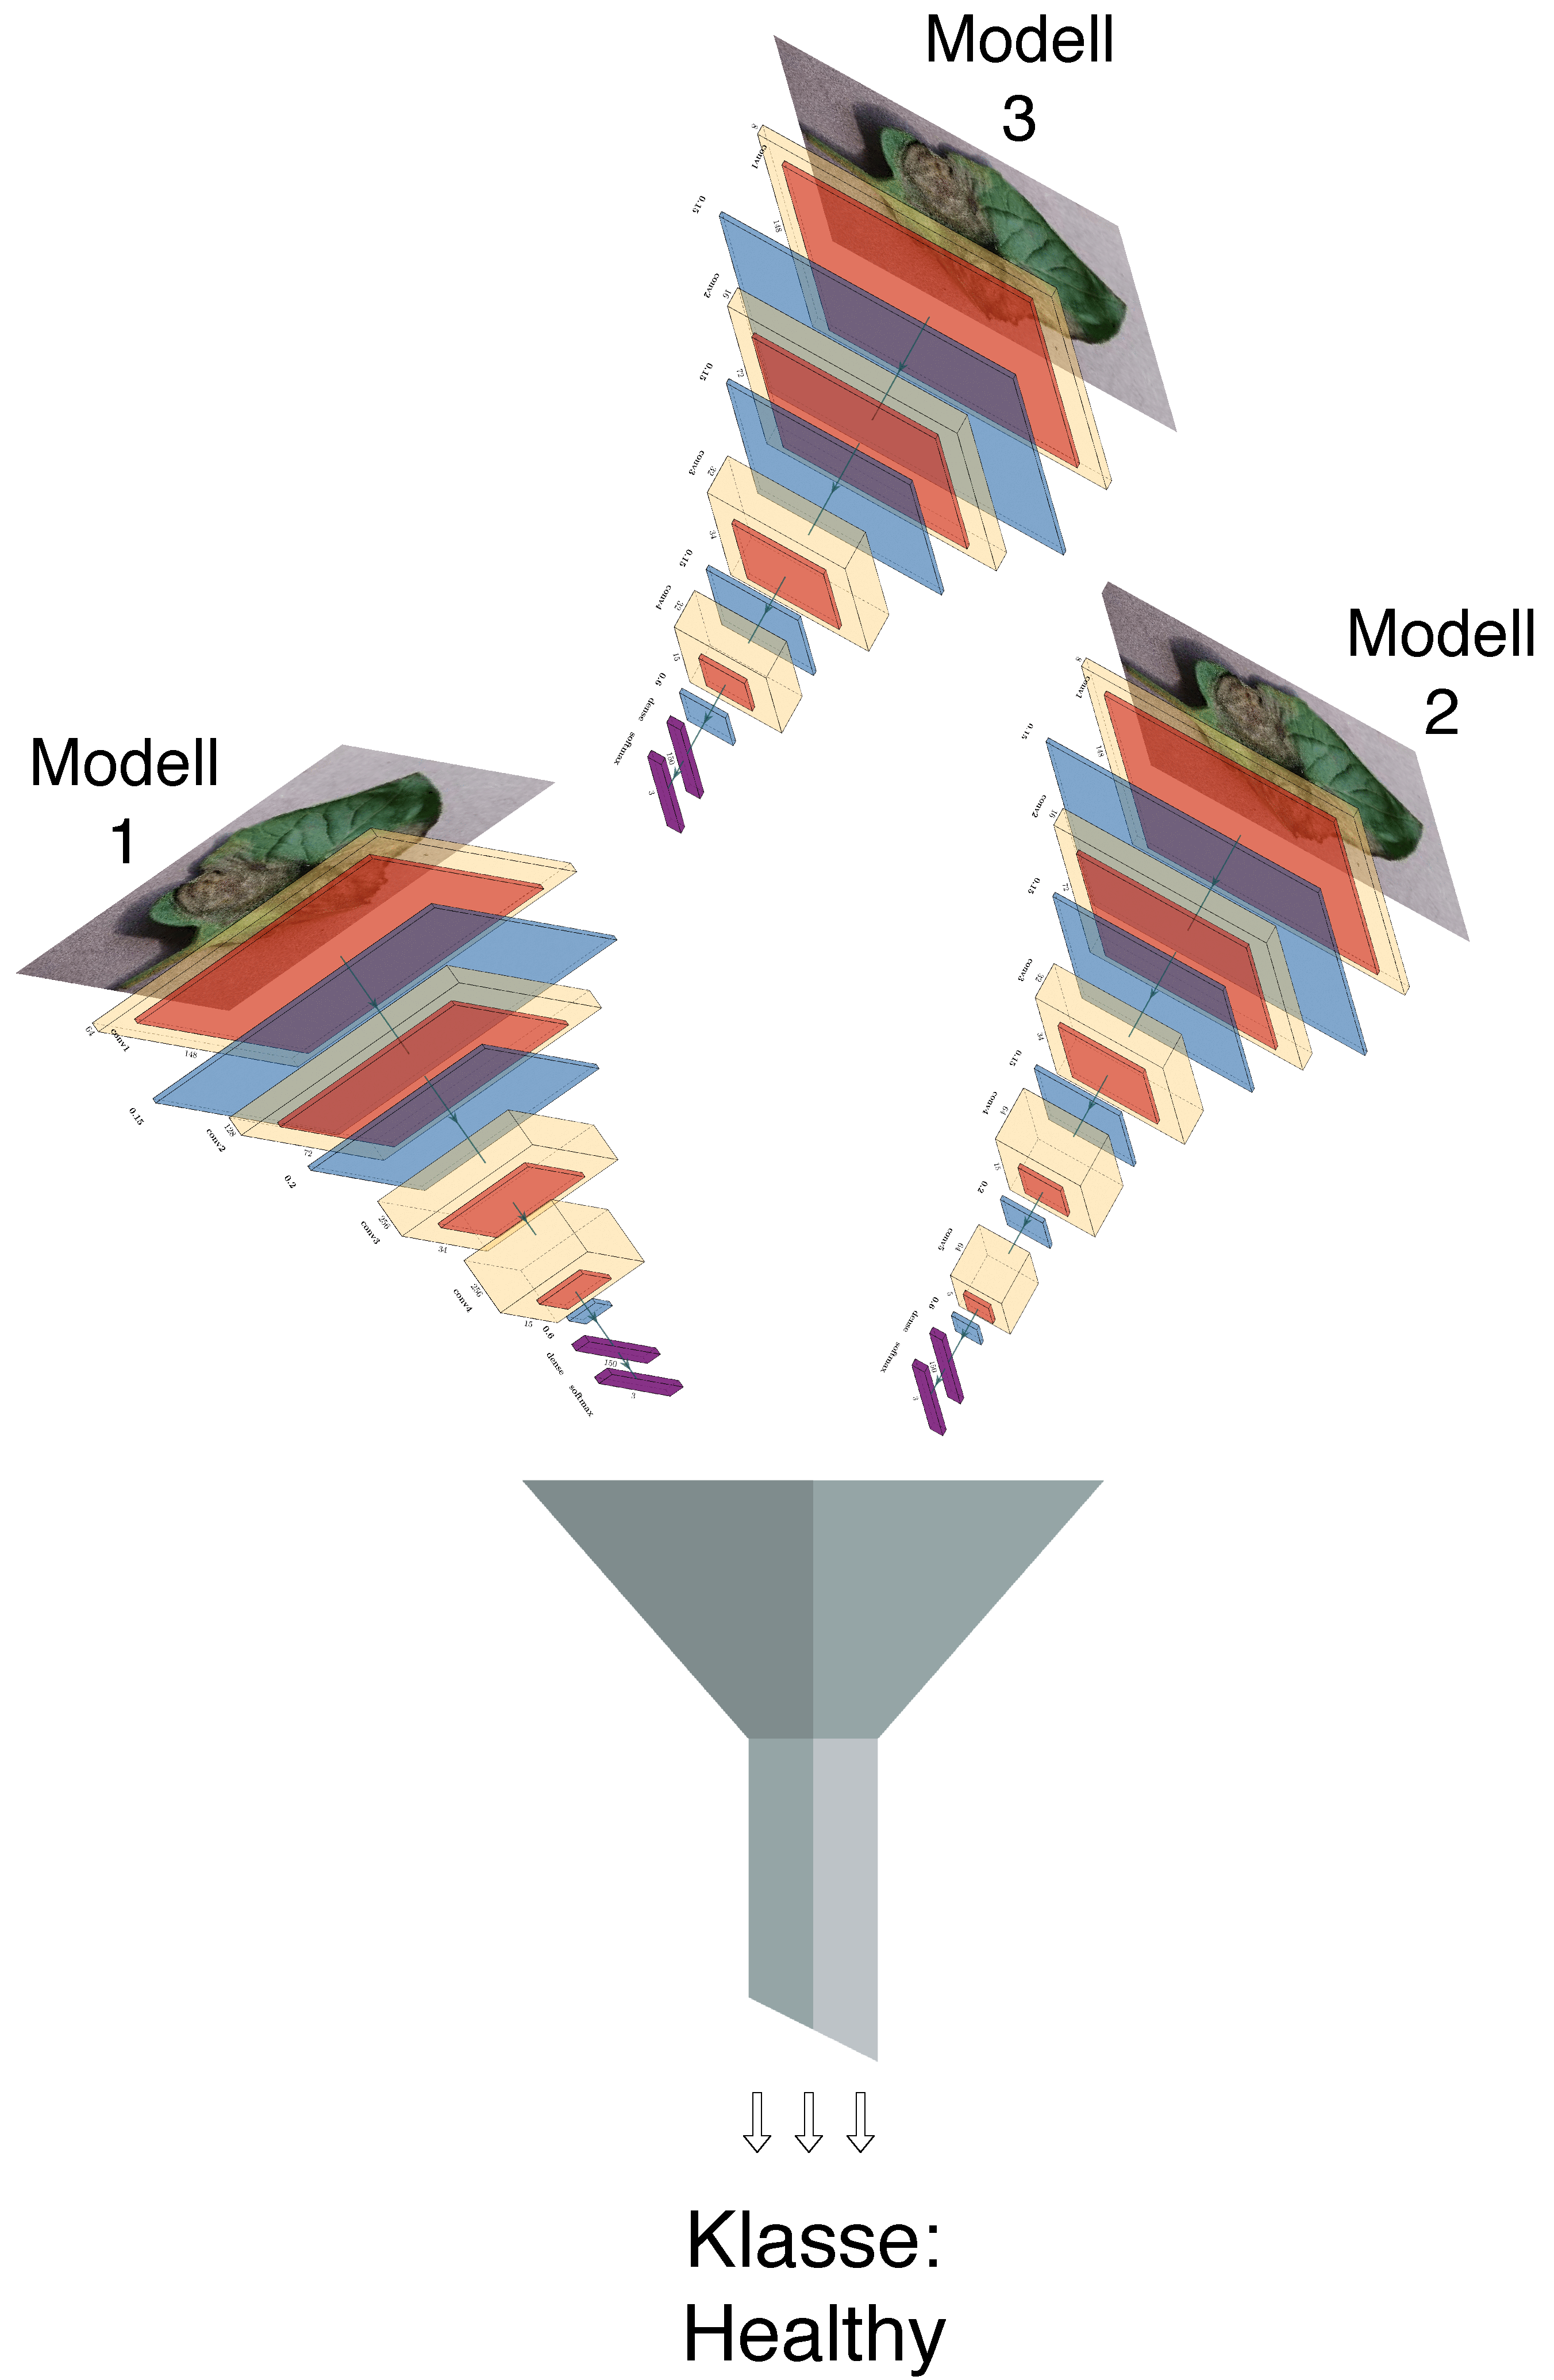
\includegraphics[width=\textwidth]{bilder/voter_image_funel.pdf}
	\caption{Darstellung eines Voters mit drei Modellen. Der Voter hat aus den Ergebnissen die Klasse \glqq Healthy\grqq~bestimmt (eigene Darstellung).}
	\label{voter_image_funel}
\end{figure}



% kapitel2.tex
\chapter{Implementierung}
\label{chapter:implementierung}

Nachdem im letzten Kapitel die Konzeption und der Entwurf einer Lösung beschrieben wurde, behandelt dieses Kapitel deren Implementierung. Im Abschnitt \ref{sec:datensatz} wird der Datensatz vorgestellt und aufbereitet. Anschließend werden in den Abschnitten \ref{sec:customNN} und \ref{sec:transferlearning} neuronale Netze mit verschiedenen Ansätzen erstellt, um die Klassifizierung der vier Krankheiten sowie gesunde Blätter zu ermöglichen. Darüber hinaus beschäftigt sich der Abschnitt \ref{sec:voter} mit drei verschiedenen, trainierten Modellen für die Klassifizierung zwischen gesunden Blättern, der Krautfäule und der Dürrfleckenkrankheit.

\section{Datensatz}
\label{sec:datensatz}
Der Datensatz stammt von einer Onlineplattform\cite{plantvillage}, die sich Pflanzengesundheit und -krankheiten widmet. Dabei sammelten die Betreiber der Plattform Daten zu Nutzpflanzen, die frei für jeden zur Verfügung stehen. Diese Daten beinhalten über 150 Pflanzenkulturen sowie 1800 Pflanzenkrankheiten. Von Pflanzenpathologen wurde der Inhalt verfasst und entspricht wissenschaftlichen Anforderungen.

Im Rahmen eines Informatikwettbewerbs von CrowdAI\cite{crowdai} zur Klassifizierung von Pflanzenkrankheiten wurde ein Datensatz erstellt, welcher einer Teilmenge des PlantVillage-Datensatzes entspricht. In der Masterarbeit werden nur die Daten aus dem Wettbewerbs-Datensatz verwendet, welcher in den folgenden Abschnitten vorgestellt wird\cite{dataset}. 

\subsection{Überblick}

Die Bilddaten wurden an experimentellen Forschungsstationen in Kooperation verschiedener staatlicher Universitäten in den USA aufgenommen\cite{dataset}.

Die Pflanzen wurden im Rahmen eines Feldversuchs mit einer Krankheit infiziert. Anschließend wurden die Blätter von Mitarbeitern entfernt und auf ein Papierblatt gelegt. Die Hintergrundfarbe des Papiers war entweder grau oder schwarz. Des Weiteren wurden alle Bilder im Freien aufgenommen. Dabei existieren Unterschiede bei der Lichtintensität. Manche Bilder wurden unter vollem Sonnenlicht und andere Bilder unter bewölkter Lichtbedingungen aufgenommen. Der Zweck hinter diesen verschiedenen Lichtintensitäten liegt darin, dass eine realistische Simulation eines Bauers, der mit dem Smartphone durch das Feld läuft und Bilder aufnimmt, dargestellt werden soll. In der Realität werden Bilder unter einer Reihe von Bedingungen aufgenommen. 

\begin{figure}[h!]
	\centering
	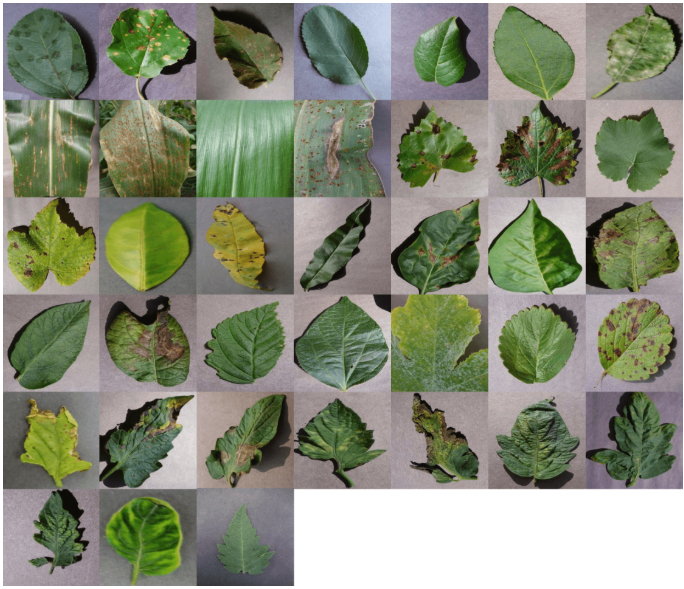
\includegraphics[width=\textwidth]{bilder/data_visualized}
	\caption{Visualisierung der verschiedenen Pflanzenkrankheiten\cite{crowdai}.}
	\label{data_visualized}
\end{figure}
Nach dem erfolgreichen Sammeln wurden die Bilder bearbeitet. Dabei wurde ein Großteil des Hintergrunds entfernt. Des Weiteren wurden die Bilder auf eine Größe von 256 x 256 Pixeln gebracht und sind so ausgerichtet, dass sie nach oben zeigen.

In der Abbildung \ref{data_visualized} werden verschiedene Pflanzen mit unterschiedlichen Krankheiten gezeigt.
In dem Datensatz sind folgende Pflanzen mit der jeweiligen Anzahl von Bilddateien vertreten: Apfel (3172), Heidelbeere (1502), Kirsche (1906), Mais (3852), Traube (4063), Orange (5507), Pfirsich (2657), Paprika (2475), Kartoffel (2152), Himbeere (371), Soja (5090), Kürbis (1835), Erdbeere (1565) und Tomate (18162). Heidelbeere, Himbeere und Soja beinhalten lediglich gesunde Bilddateien. Bei den Pflanzen Orange und Kürbis liegen nur Bilddateien vor, die kranke Blätterausprägungen zeigen. Insgesamt treten in diesem Datensatz 26 Pflanzenkrankheiten auf.

%TODO: Text im Plot größer! Nochmal neu machen!
\begin{figure}[h!]
	\centering
	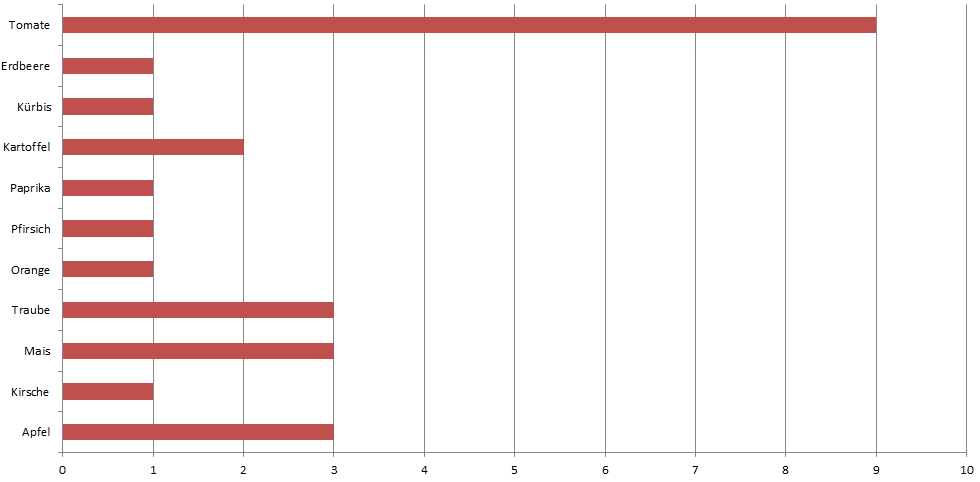
\includegraphics[width=\textwidth]{bilder/disease_distribution}
	\caption{Verteilung der Krankheiten auf Pflanzen (eigene Darstellung).}
	\label{disease_distribution}
\end{figure}

Davon sind 17 Pilzerkrankungen, vier bakteriellen Erkrankungen, zwei Schimmelpilzerkrankungen, zwei Viruserkrankungen und eine Erkrankung durch eine Milbe. In der Abbildung \ref{disease_distribution} wird die Verteilung der jeweiligen Krankheiten auf die Pflanzen veranschaulicht. Dabei sticht die Tomate besonders hervor, da neun Pflanzenkrankheiten in diesem Datensatz zu finden sind.

\begin{figure}[h!]
	\centering
	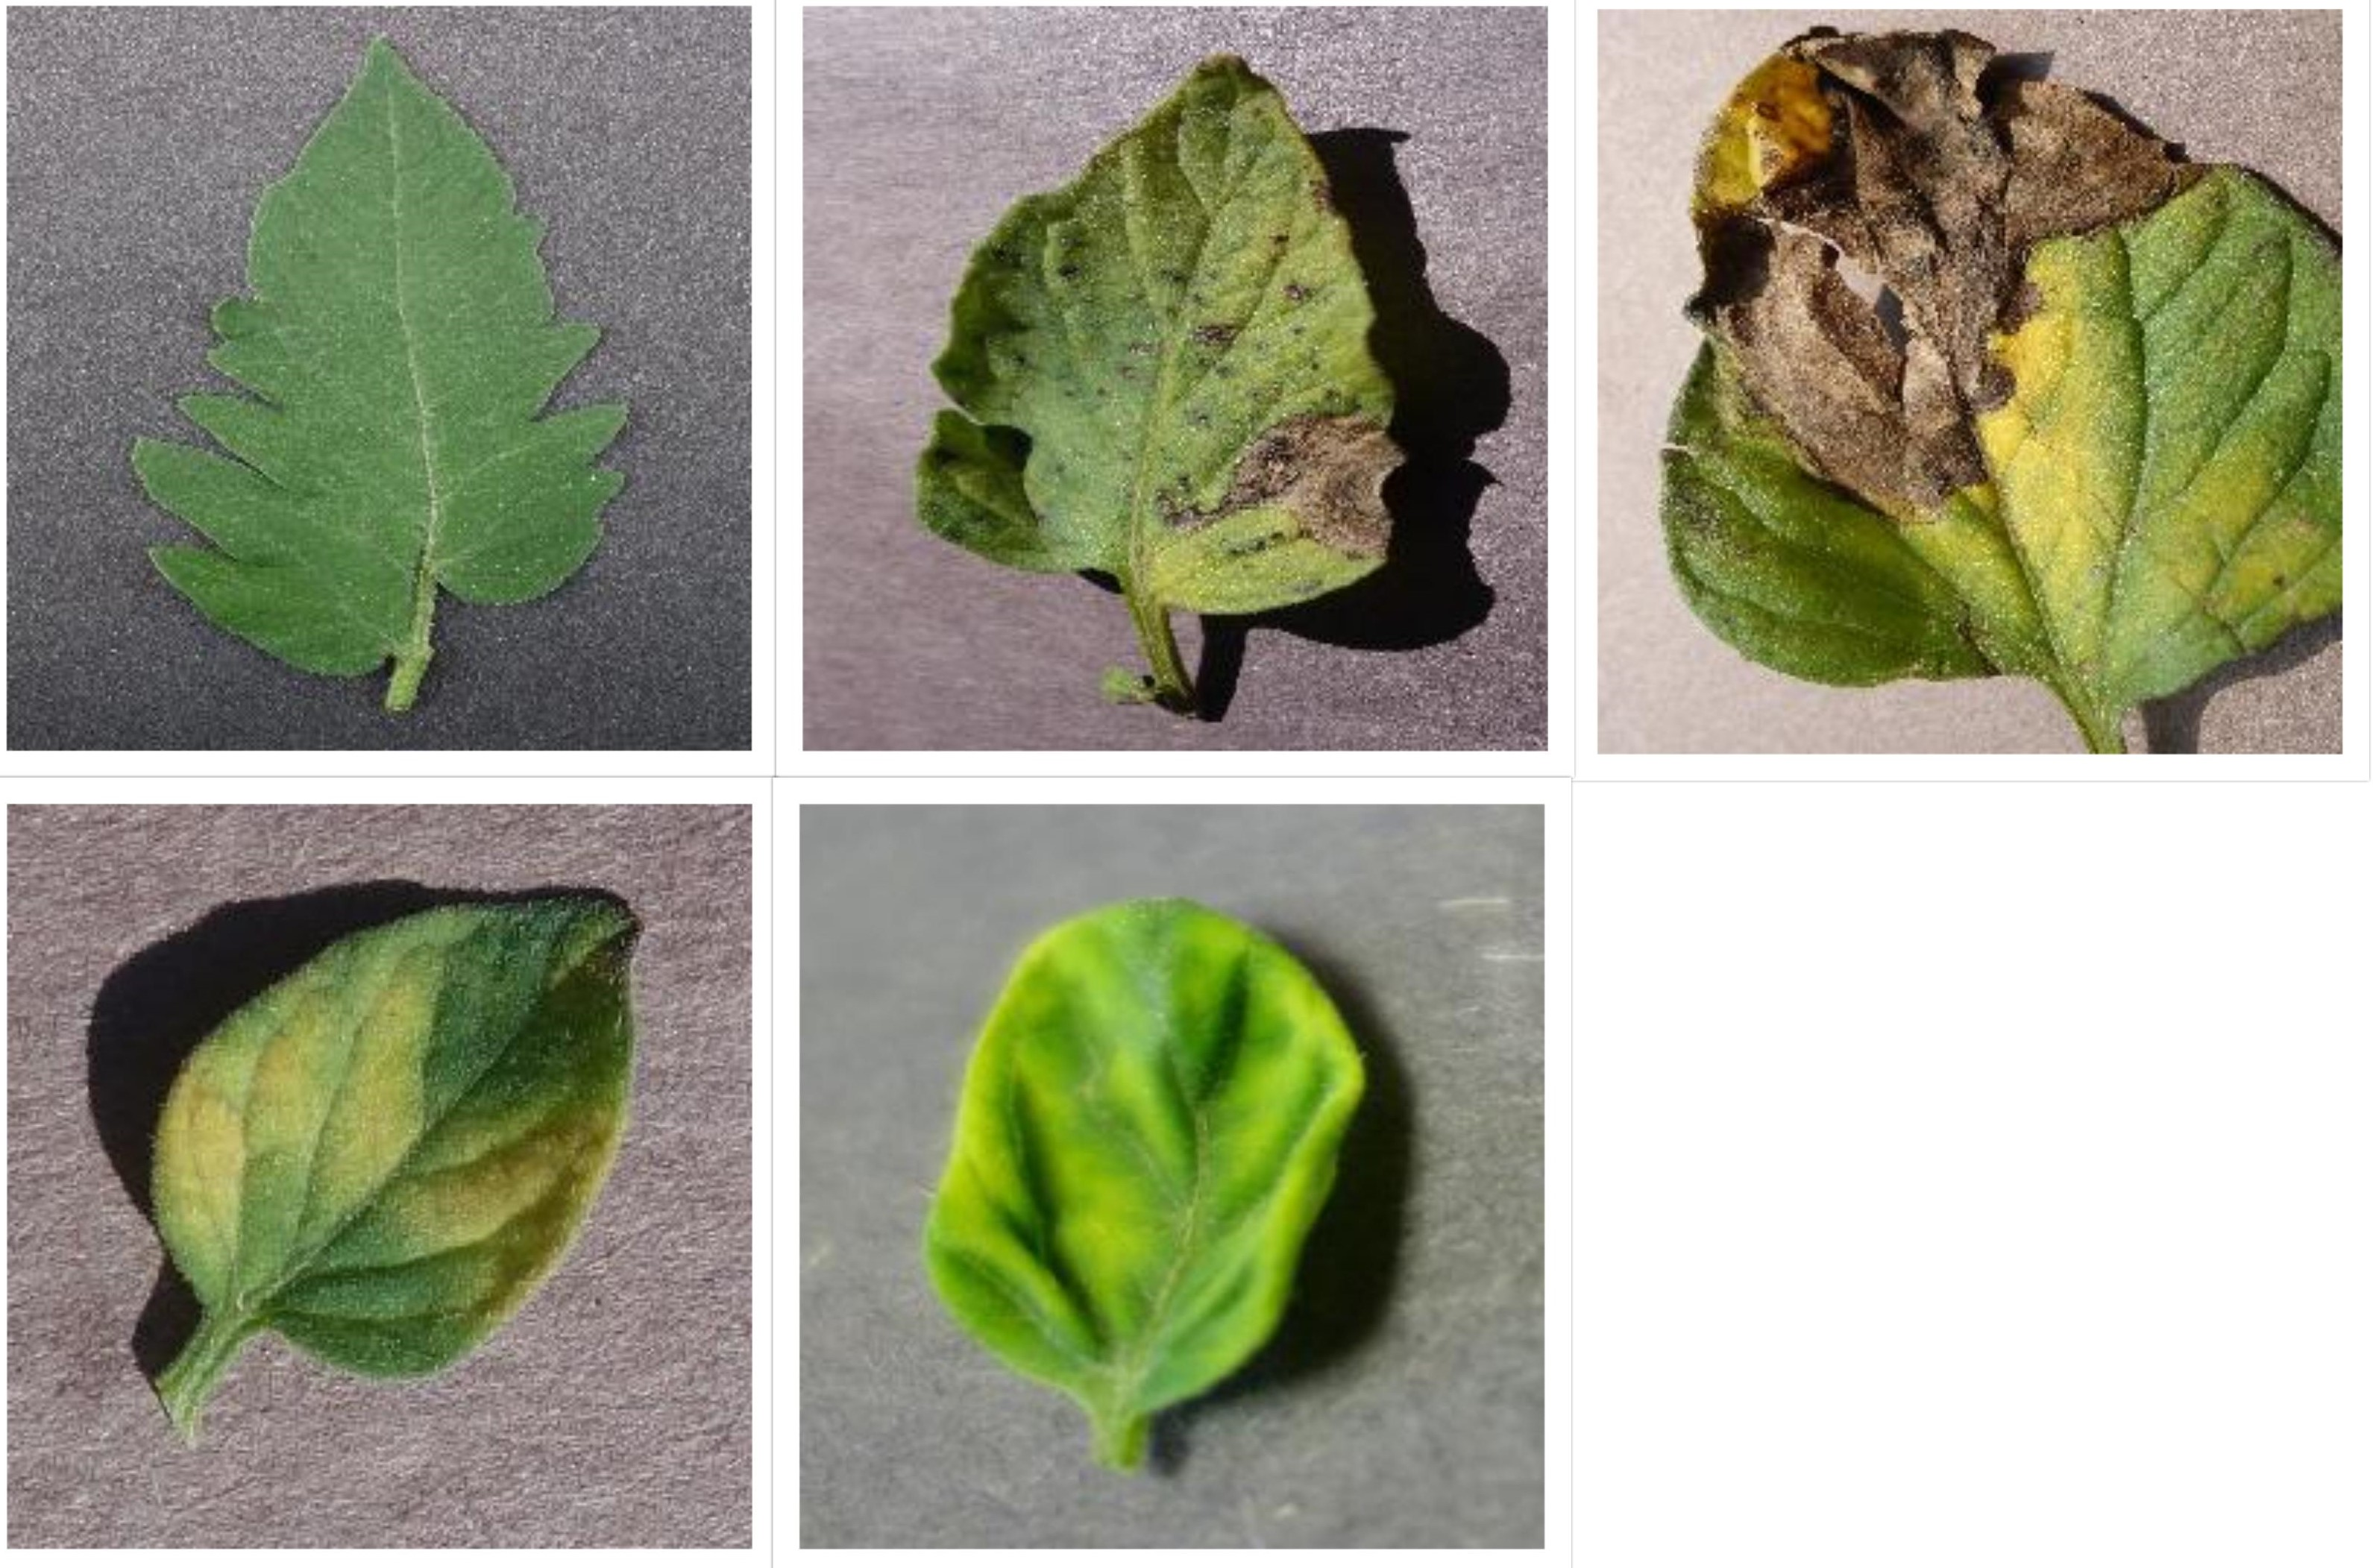
\includegraphics[width=0.8\textwidth]{bilder/collage_5_classes}
	\caption{Visualisierung der fünf Krankheiten, die in dieser Arbeit untersucht wird (eigene Darstellung).}
	\label{collage_5_classes}
\end{figure}


In dieser Masterarbeit wird nur ein Ausschnitt aus dem gegebenen Datensatz behandelt. Fünf Klassen, nämlich \glqq Healthy\grqq, \glqq Early Blight\grqq, \glqq Late Blight\grqq, \glqq Leaf Mold\grqq~und \glqq Yellow Leaf Curl Virus\grqq, werden in der Abbildung \ref{collage_5_classes} beginnend mit der gesunden Tomate von links nach rechts dargestellt. 


\subsection{Aufbereitung}


Neuronale Netze benötigen bestimme Vorverarbeitungsschritte, um gute Ergebnisse liefern zu können. Des Weiteren muss die Struktur des Datensatzes angepasst werden, so dass das Lernverfahren durchführbar ist. 

\subsubsection{Teilung des Datensatzes}
%Quelle wegen den Hauptspeicher
\begin{figure}[!h]
	\begin{minipage}[c]{0.5\textwidth}
		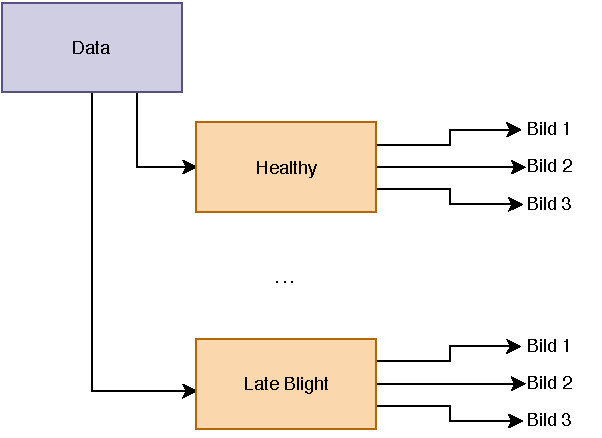
\includegraphics[width=\textwidth]{bilder/original_structure}
		\caption{Die Struktur von dem Datensatz (eigene Darstellung).}
		\label{original_structure}
	\end{minipage}
	\hfill
	\begin{minipage}[c]{0.48\textwidth}
	Der Datensatz hat für jede Klasse einen Ordner. Alle Bilddateien zu einer Klasse befinden sich dementsprechend in einem Ordner. Die Abbildung \ref{original_structure} zeigt die Struktur von dem Datensatz. Für das Trainingsverfahren des neuronalen Netzes wird der Datensatz in Trainings-, Validierungs- und Testsdateien aufgeteilt. Die Abbildung \ref{flow_chart} veranschaulicht die Struktur des Datensatzes, die für die nächsten Schritte benötigt werden.
	\end{minipage}
\end{figure}


Der Vorteil an dieser Strukturierung ist, dass der komplette Datensatz nicht in den 
\begin{figure}[h!]
	\centering
	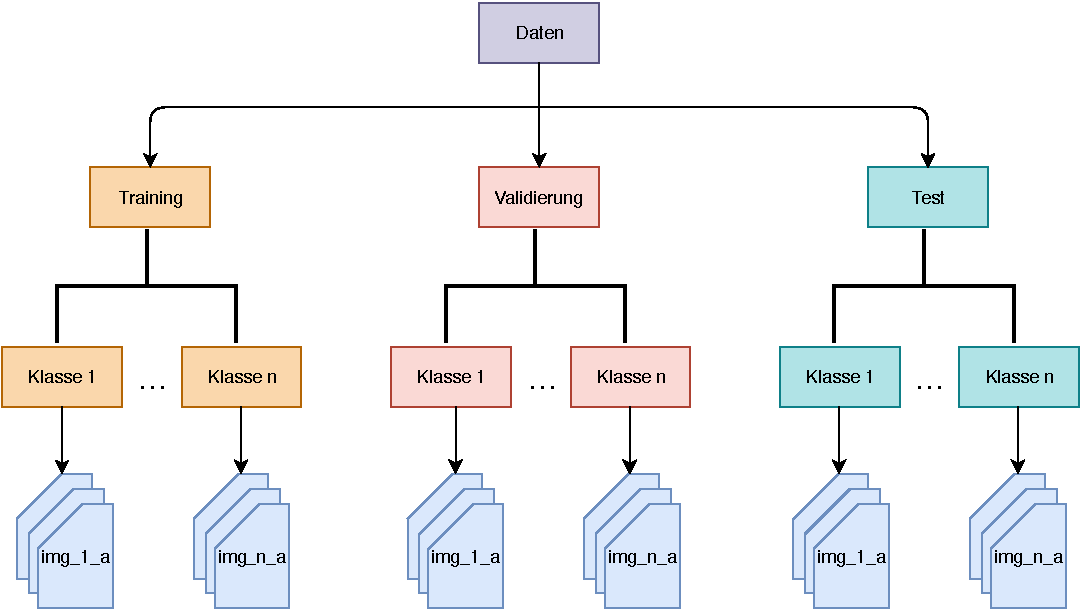
\includegraphics[width=0.73\textwidth]{bilder/flow_chart}
	\caption{Die Darstellung der angepassten Ordnerstruktur, die in drei Teilordner, hier Training, Validierung und Test, aufgeteilt wurde (eigene Darstellung).}
	\label{flow_chart}
\end{figure}

 \newpage~\newline
Hauptspeicher geladen werden muss. Sehr große Datensätze können im schlimmsten Fall nicht im Hauptspeicher passen. Die Bibliothek Keras bietet daher eine Klasse an, die das Einlesen der Daten übernimmt. Die Klasse \textit{ImageDataGenerator}\cite{flowfrom} liest schrittweise die Daten ein. Dabei werden die Daten stapelweise (engl. Batch) eingelesen, so dass kleinere sowie sehr große Datensätze verwendet werden können. Es werden nur so viele Daten in den Hauptspeicher geladen, wie für den aktuellen Batch beim Training und der Validierung des Modells benötigt werden.

\subsubsection{Anpassung der Verteilung}

CNNs haben in der Praxisanwendung Probleme, wenn einige Klassen eine deutlich höhere Anzahl an Daten in dem Trainingsdatensatz als andere Klassen haben. Dieses Klassenungleichgewicht sorgt für Schwierigkeiten bei dem Lernverfahren von klassischen Klassifikatoren und mehrschichtigen neuronalen Netzen. Dabei wirkt es sich die Konvergenz während der Trainingsphase aus und könnte die Generalisierung des Modells bei dem Testdatensatz negativ beeinflussen. Eine naive, leichte Lösung des Problems ist das Undersampling. Mit dieser Methodik wird zufällig ein Teil der Daten aus den überrepräsentierten Klassen entfernt\cite{papernn}.

\begin{figure}[h!]
	\centering
	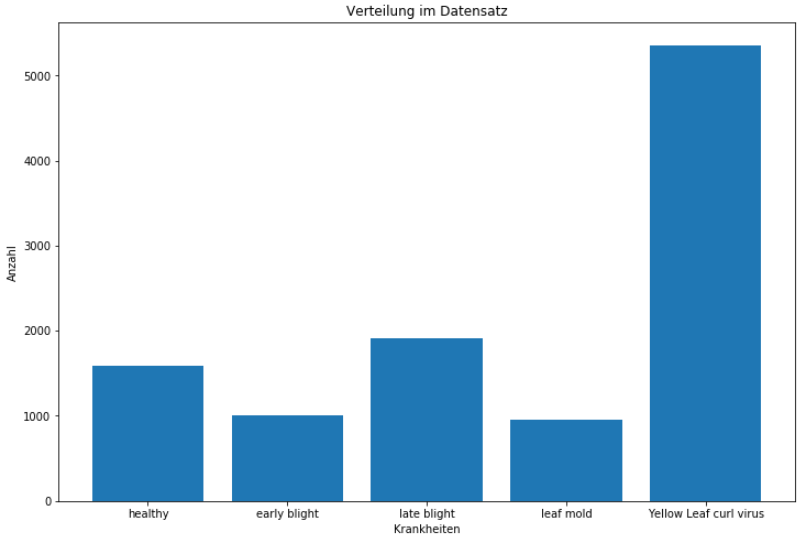
\includegraphics[width=\textwidth]{bilder/original_distribution.PNG}
	\caption{Die Verteilung der Daten ist bei den Klassen nicht gleich verteilt. Die Datenmenge von der TYLCV-Krankheit ist mindestens doppelt so groß im Vergleich zu den anderen Krankheiten (eigene Darstellung).}
	\label{original_distribution}
\end{figure}

In der Abbildung \ref{original_distribution} wird die momentane Verteilung der Daten von vier verschiedenen Pflanzenkrankheiten sowie der gesunden Klasse veranschaulicht. Hierbei ist klar zu sehen, dass die Klasse \glqq TYLCV\grqq~mit über 5000 Bilddaten deutlich überrepräsentiert ist. Die anderen Klassen haben eine Datenmenge zwischen 800 und 2000 Bildern. Daher wird hier der naive Ansatz angewendet, um alle Datenmengen jeweiliger Klasse auf den Bereich 700 bis 800 zu reduzieren. Die Trainingsdaten der Klasse \glqq TYLCV\grqq~werden drastisch gekürzt. Des Weiteren wurden die beiden leicht überrepräsentierten Klassen \glqq healthy\grqq~und \glqq leaf mold\grqq~auch gekürzt. Nun befindet sich die Menge von Trainingsdaten aller Klassen in der Spannweite zwischen 700 und 800 (s. Abbildung \ref{corrected_distribution}). Außerdem wurde in dieser Abbildung die Anzahl der Validierungs- und Testdaten in orange und grün gekennzeichnet. Die Menge an Validierungsdaten liegt zwischen 150 bis 300. Die Testdaten sind im Vergleich zu den anderen Daten deutlich geringer, nämlich zwischen 80 bis 280.

\begin{figure}[h!]
	\centering
	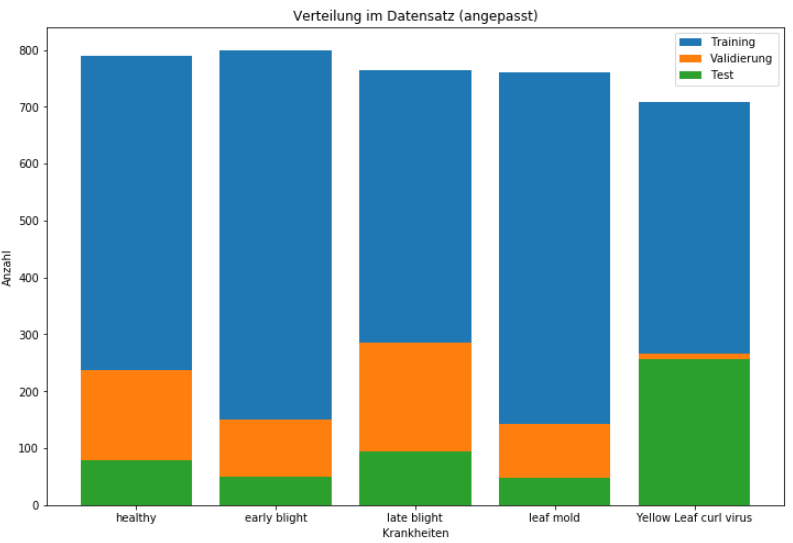
\includegraphics[width=\textwidth]{bilder/corrected_distribution.PNG}
	\caption{Die Anzahl der Trainingsdaten von allen Klassen (blau) befindet sich in dem Bereich zwischen 700 und 800. Die orangene Säule repräsentiert die Validierungsdaten, dessen Anzahl maximal 280 liegt. Außerdem stellt die grüne Säule die Testdaten dar, die bei der Klasse \glqq TYLCV\grqq~leicht höher ist (eigene Darstellung).}
	\label{corrected_distribution}
\end{figure}


\subsubsection{Vorverarbeitung}

%load the data from the directory on demand with the help of flow_from_directory in Keras
% https://keras.io/preprocessing/image/#imagedatagenerator-class

Da der Datensatz nicht vorverarbeitet ist, werden Vorverarbeitungen benötigt, um den Datensatz optimal für den Lernprozess vorzubereiten. Zunächst wird der Datensatz künstlich erweitert, um eine Anzahl von Variationen zu erzeugen. Damit kann eine Überanpassung des Modells verhindert werden. Der Gradbereich für zufällige Rotationen liegt bei maximalen 40 Grad. Darüber hinaus werden die Bilder horizontal und vertikal in beide Richtungen zufällig bis 20\% verschoben. Außerdem werden die Bilder im Gegenuhrzeigersinn um 20\% geschert. Um weitere Diversität in dem Datensatz zu erzeugen, werden die Bilder mit dem Faktor 30\% rein- sowie rausgezoomt. Die durch Transformation entstandenen Flächen werden mit dem Farbton des angrenzenden Pixels gefüllt. Ein weiterer Vorverarbeitungsschritt ist nun das zufällige, horizontale Spiegeln der Bilder. Anschließend werden die Farbwerte normiert. Da jeder Farbkanal jeweils acht Bit lang ist, ist der maximale Wert bei 256. Daher werden die Farbwerte durch 255 geteilt, um den Zahlenbereich der RGB-Werte zwischen null und eins zu erhalten. 

In Abbildung \ref{data_segm} werden drei Bilder gezeigt. Das linke Bild ist das unverarbeitete Bild aus dem Datensatz. Die Bilder, die sich in der Mitte sowie rechts befinden, wurden mit verschiedenen Transformationen geändert. Das mittlere Bild ist horizontal gespiegelt und die Blattfläche nimmt mehr Platz in dem Bild ein. Deutlich ist es zu erkennen, dass das rechte Bild herausgezoomt wurde. Daher hat dieses Bild einige geradlinige Füllelemente.  

%Vorher und nachher Vergleich
\begin{figure}[h!]
	\centering
	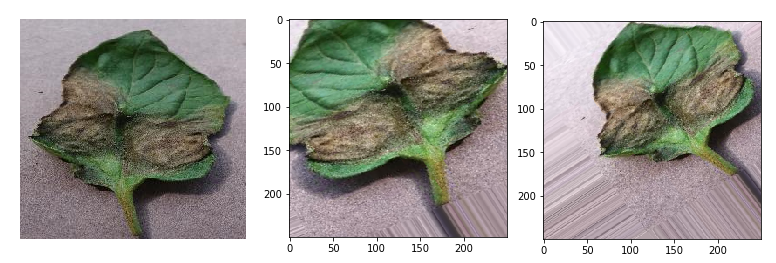
\includegraphics[width=\textwidth]{bilder/data_segmentation.PNG}
	\caption{Das linke Bild zeigt das unveränderte Bild. Durch Transformationen wird das mittlere sowie rechte Bild verändert. Des Weiteren wurden die Farbweite von den beiden Bildern normalisiert.}
	\label{data_segm}
\end{figure}

\section{Anmerkungen zum Training}
%Titel ändern??

Aus Übersichtlichkeitsgründen wird ein Teil der Hyperparameter für alle folgenden Modelle hier zusammengefasst, da sie größtenteils redundant sind. Bei allen Modellen greift das Modell auf die kategorische Kreuzentropie als Kostenfunktion zurück, da das Klassifizierungsproblem mehr als zwei Klassen beinhaltet. Des Weiteren werden die neuronalen Netze mithilfe von dem Gradientenabstieg des Typs \glqq Adam\grqq~trainiert. Hierbei ist die Lernrate auf den Wert 0.001 gesetzt. Die Größe des Batchs liegt bei 230. 

Unterschiede zwischen den Modellen liegen bei der Anzahl der Epochen oder der Konfiguration des frühzeitigen Abbruchs des Trainings.

\section{Aufbau des neuronalen Netzes}
\label{sec:customNN}
%Chapter Titel anpassen?
%Convolution und poolingschicht schreibweise nochmal überprüfen

Das hier vorgestellte neuronale Netz soll die vier Krankheiten und zusätzlich gesunde Blätter erkennen, die im Abschnitt \ref{sec:Blattkrankheiten} vorgestellt wurden.  

%Modell
%\subsection{Struktur}
Das Modell hat eine grundlegende Struktur. Nach jeder Faltungsschicht folgt unmittelbar eine Max-Poolingschicht. Insgesamt treten solche Konstrukte fünf mal auf. Anschließend beinhaltet das Modell zwei weitere voll verbundene Schichten. Grundsätzlich haben alle Filter in den Faltungsschichten die Größe 3 x 3 und werden mit der ReLU-Aktivierungsfunktion aktiviert. Die Fenstergröße der Poolingschichten ist auf die Größe 2 x 2 gesetzt.
In Abbildung \ref{my_arch} wird die Struktur des Modells visualisiert. Gelbe Flächen sollen Faltungsschichten, rote Poolingsschichten und blaue dementsprechend Dropout-Schichten symbolisieren. Zunächst wird das Modell mit einer Faltungsschicht, die das Eingangsbild in der Größe 150 x 150 akzeptiert, beginnen. Das Eingangsbild wurde von der ursprünglichen Größe von 256 x 256 auf 150 x 150 verkleinert, um in der Lernphase Zeit zu sparen. Die Anzahl der Filter in der ersten Faltungsschicht beträgt 32.

\begin{figure}[h!]
	\centering
	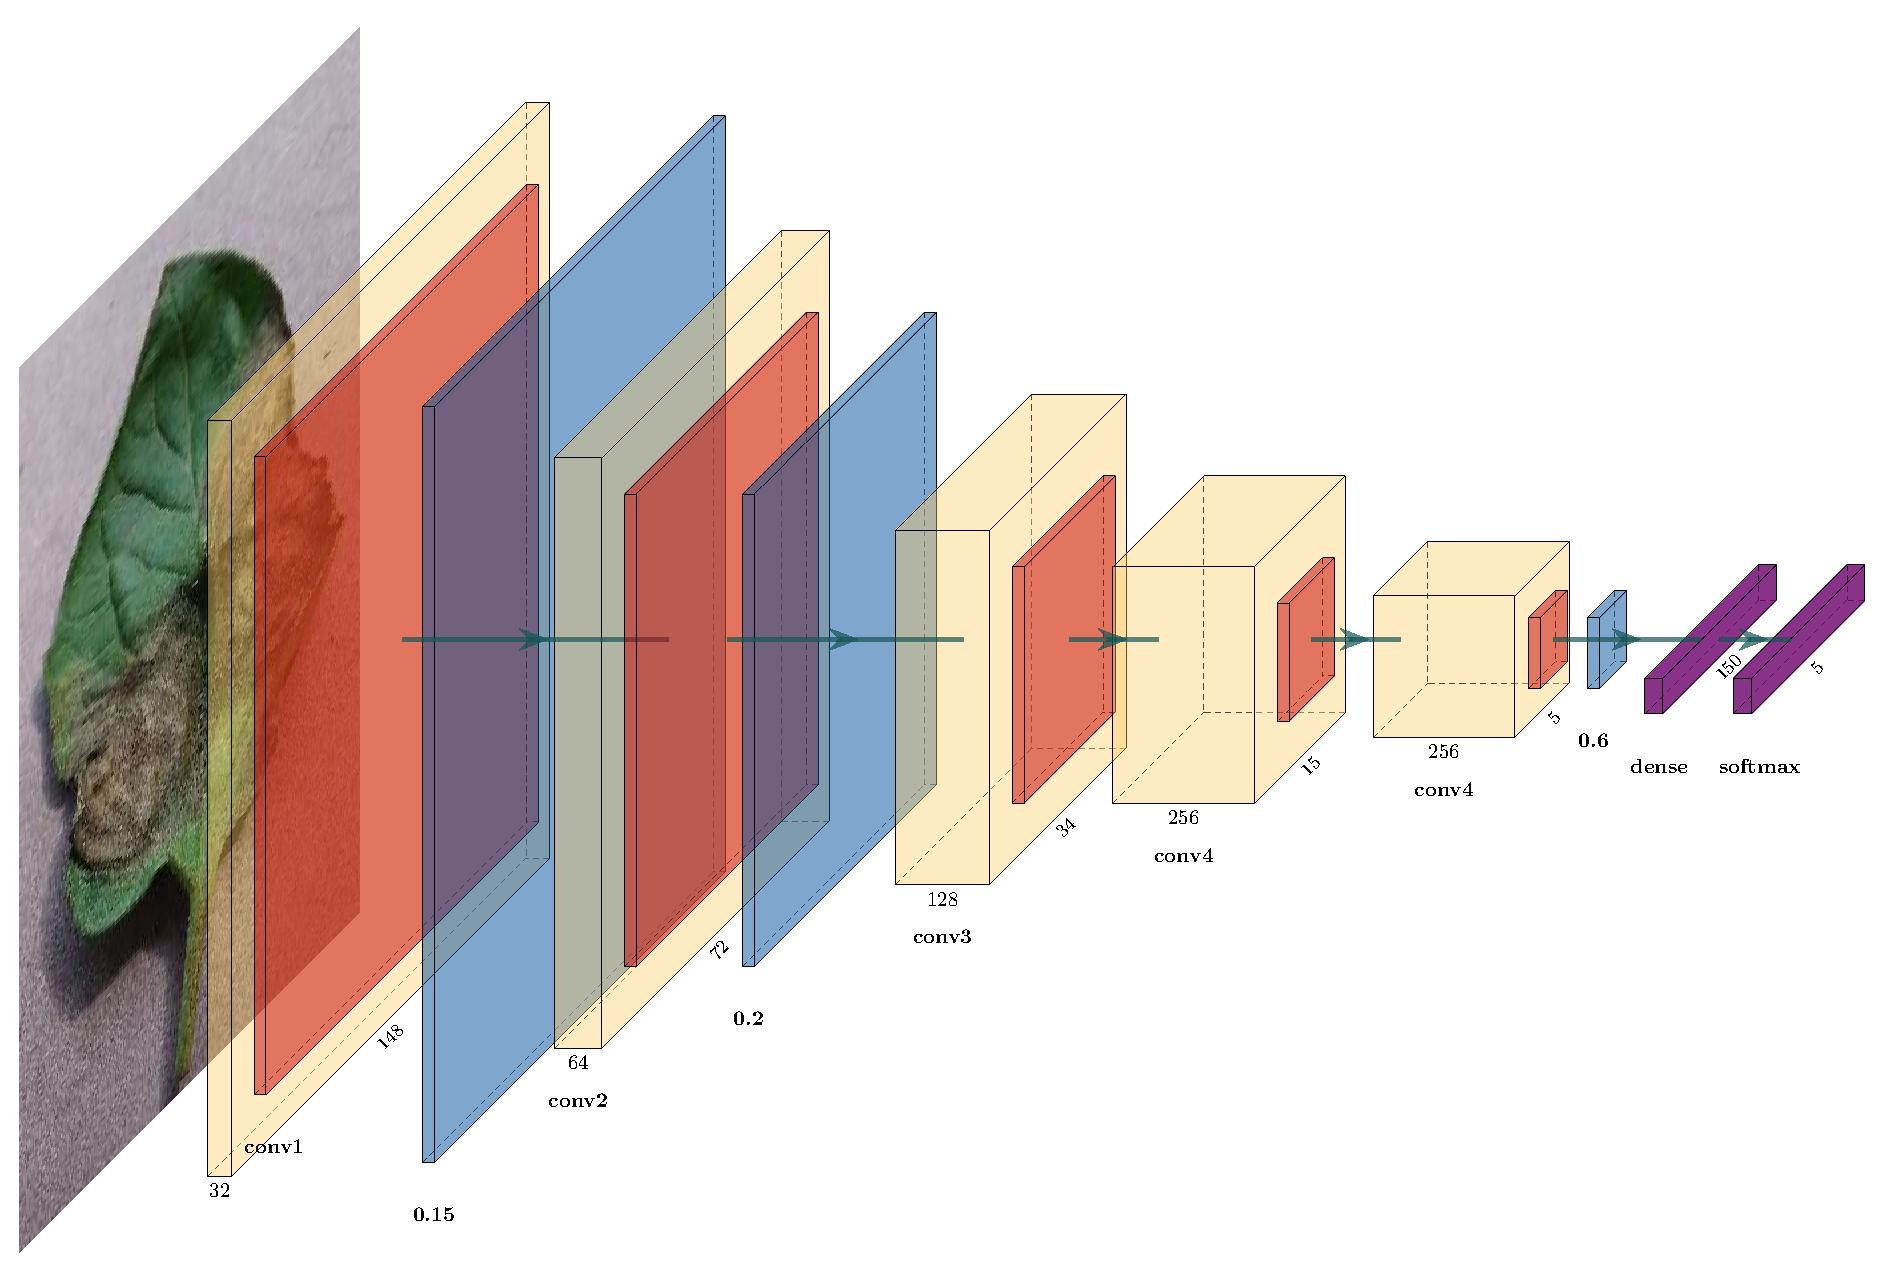
\includegraphics[width=\textwidth]{bilder/my_arch.pdf}
	\caption{Darstellung des Modells mit fünf Faltungs- und Poolingschichten (eigene Darstellung).}
	\label{my_arch}
\end{figure} 
 
Nach der ersten Max-Poolingschicht folgt die erste Dropout-Schicht mit dem Wert 0.15. Anschließend folgt die zweite Faltungsschicht mit 64 Filtern. Auch hier wird nach der zweiten Max-Poolingschicht eine zweite Dropout-Schicht hinzugefügt, um 20\% der Ausgabefunktionen auf den Wert 0 setzen zu können. Die dritte Faltungsschicht hat insgesamt 128 Filter. Anknüpfend werden zwei weitere Faltungsschichten mit ihren Max-Poolingschichten im Modell hinzugefügt. Hierbei beträgt die Anzahl der Filter bei beiden Schichten 256. Daraufhin fügt sich eine Dropout-Schicht an, die auf 60\% eingestellt ist. Nach der letzten Dropout-Schicht weist das Modell zwei voll verbundene Schichten auf, wobei die erste Schicht 150 Knoten und die ReLU-Aktivierungsfunktion hat. Außerdem werden die Gewichte dieser Schicht mit einer L2-Regularisierung mit dem Faktor 0.002 angepasst. Die zweite voll verbundene Schicht hat nur fünf Knoten, da nur fünf Klassen klassifiziert werden sollen. Um die Klassifikation durchführen zu können, wird auf die Softmax-Aktivierungsfunktion zurückgegriffen. 




\paragraph{Training}
~\newline

Das Modell wird mit 200 Epochen trainiert. Dabei kann das Training frühzeitig abgebrochen werden, wenn sich die Kosten des Validierungsdatensatzes nicht minimieren. Bevor der Abbruch stattfindet, werden zunächst 20 Epochen durchlaufen. Hierbei stellt sich heraus, ob die Kostenfunktion einen neuen minimalen Wert zurückgibt. Das Trainingsverfahren bricht bei der Hälfte, hier bei der 96. Epoche, schon ab. Das beste Modell bezüglich der minimalen Kosten wurde in der 76. Epoche erreicht und hat eine Genauigkeit von 98.51\%.







\section{Voter}
\label{sec:voter}
%- performance des Voters im  kapitel eval
Um die Anzahl der Fehlklassifizierungen reduzieren zu können, wird in diesem Abschnitt auf einen Voter gesetzt. Die Grundidee hierbei ist, dass mehrere Modelle dasselbe Eingangsbild erhalten und klassifizieren. Der Voter wählt aus den Ergebnissen der drei verschiedenen trainierten Modelle die passende Klasse aus. Hierbei wird die Klasse, die am häufigsten unter den drei Modellen erkannt wurde, ausgewählt. Die folgenden Modelle wurden speziell für die zwei Krankheiten, hier Dürrfleckenkrankheit und Krautfäule, entworfen. Daher kann der Voter zwischen diesen beiden Krankheiten sowie gesunden Blättern auswählen.


\subsection{Modell 1}
\label{model1_voter}
%\subsubsection{Struktur}
Das vorliegende Modell sowie alle anderen folgenden Modelle beinhalten denselben Aufbau. Auf jede Faltungsschicht folgt eine Max-Poolingschicht. Diese Kombination tritt genau vier Mal auf. Zwei voll verbundene Schichten runden die Architektur des Modells ab. Auch hier ist die Filtergröße der Faltungsschichten 3 x 3 groß und sind mit der ReLU-Aktivierungsfunktion eingestellt. Die Größe des Max-Poolingfenster beträgt  2 x 2. Diese Parametergrößen sind bei den folgenden Modellen in den Abschnitten \ref{model2_voter} und \ref{model3_voter} dieselben. 
Die erste Faltungsschicht mit 64 Filtern akzeptiert das Eingangsbild, das in der Größe 150 x 150 vorliegt. Anschließend wurde nach der Max-Poolingschicht eine Dropout-Schicht hinzugefügt, welche 15\% der Ausgabefunktionen nicht mehr beachtet. Nach einer solchen Dropout-Schicht wird eine Kombination aus einer Faltungsschicht mit der doppelten Anzahl von Filtern und einer Max-Poolingschicht gesetzt. Daraufhin folgt wieder eine Dropout-Schicht, die auf 20\% eingestellt ist. Nach dieser Schicht wird die Architektur mit zwei Kombinationen aus einer Faltungschicht mit 256 Filtern und einer Max-Poolingschicht erweitert. Nach der Erweiterung wird eine letzte Dropout-Schicht mit der Rate von 60\% ergänzt, so dass zwei voll verbundene Schichten mit 150 sowie fünf Knoten vervollständigt werden können. Die erste voll verbundene Schicht weist die ReLU-Aktivierungsfunktion auf. Die Gewichte in dieser Schicht werden mit dem Faktor 0.002 mittels einer L2-Regularisierung korrigiert. Die zweite voll verbundene Schicht ist mit einer Softmax-Aktivierungsfunktion versehen, um die drei Klassen bestimmen zu können.        


\begin{figure}[h!]
	\centering
	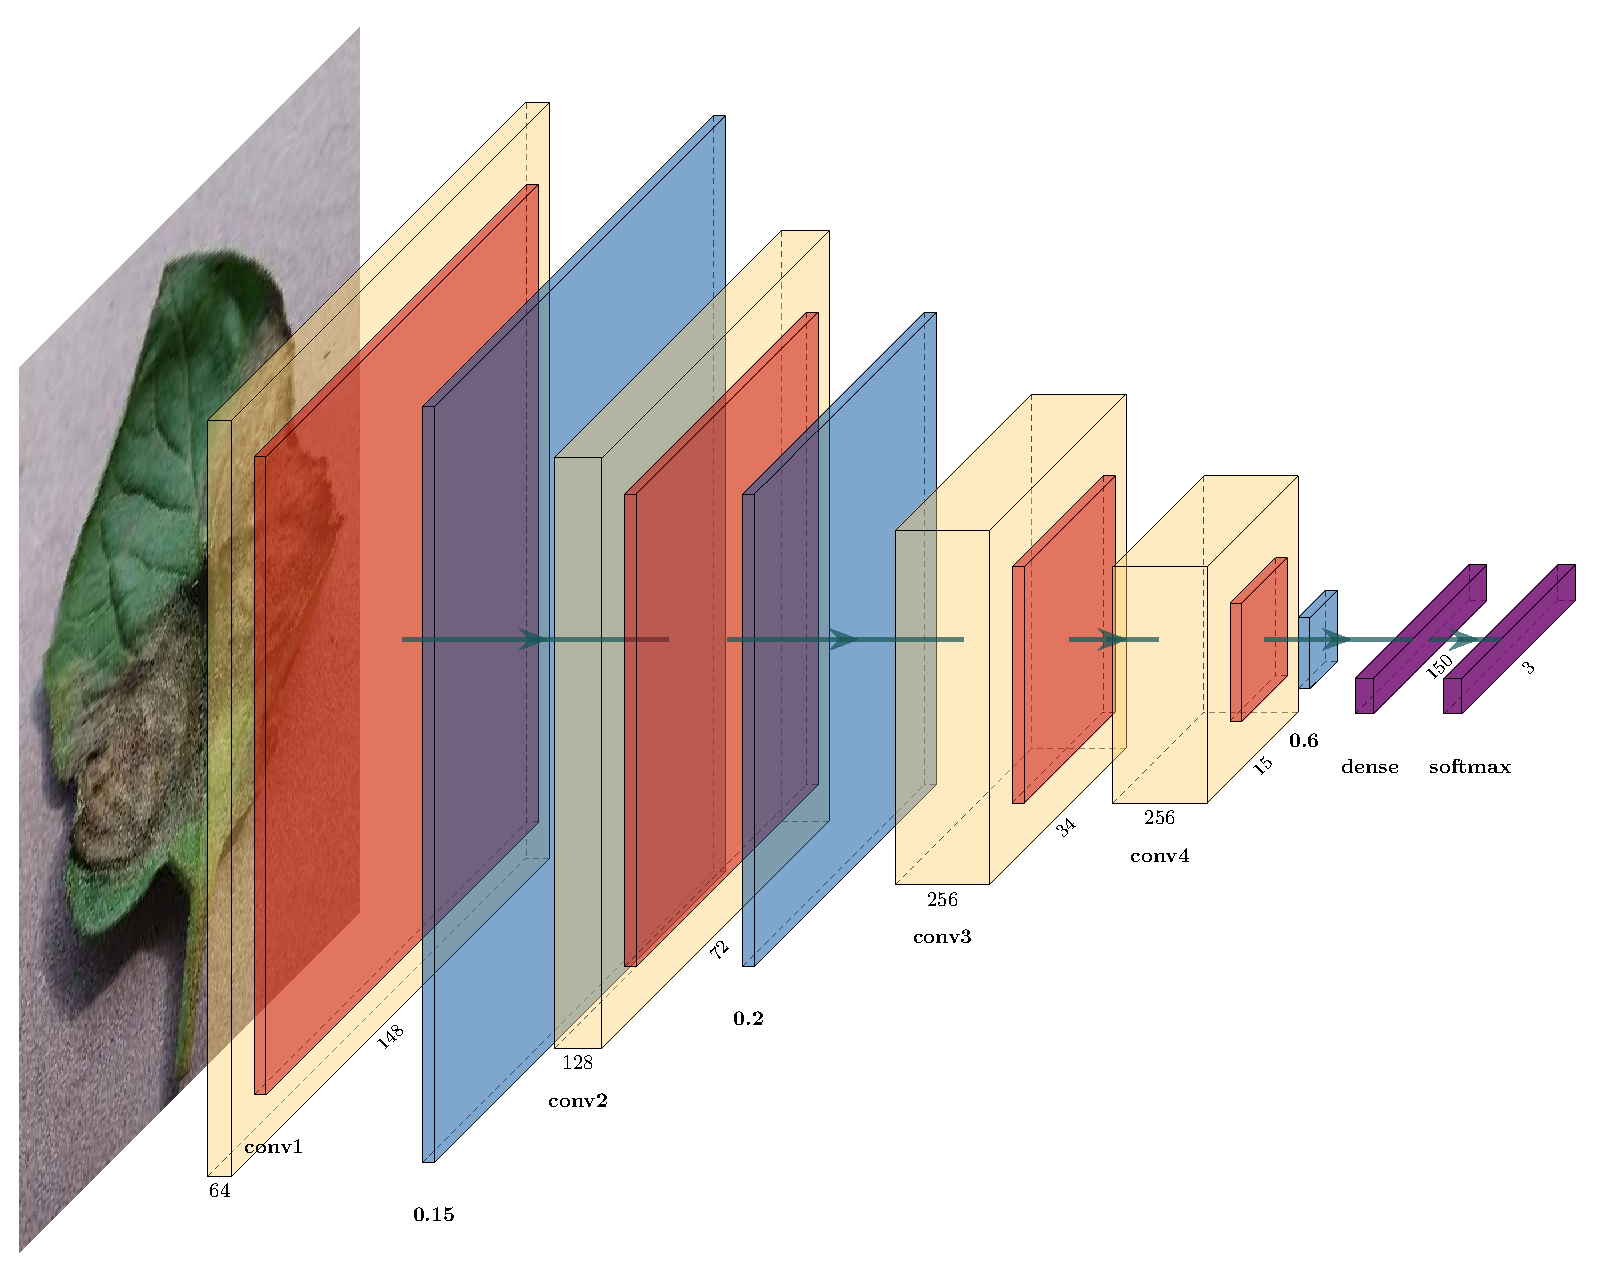
\includegraphics[width=\textwidth]{bilder/voter1.pdf}
	\caption{Veranschaulichung des ersten Modells mit vier Faltungs- und Poolingschichten und drei Dropout-Schichten (eigene Darstellung).}
	\label{voter1}
\end{figure}

\newpage
\paragraph{Training}
~\newline

Dieses Modell erreicht schnell gute Ergebnisse. Schon bei der 35. Epoche von 100 wurden die minimalsten Kosten erreicht und das Modell weist bei weiteren Epochen keine Verbesserungen auf. Deswegen wird das Training nach 15 weiteren Epochen abgebrochen. Die Genauigkeit des Modells liegt bei 97.94\%. 


\subsection{Modell 2}
\label{model2_voter}
%\subsubsection{Struktur}

Dieses Modell setzt auf viele Faltungsschichten mit einer kleinen Anzahl von Filtern. Die erste Faltungsschicht hat lediglich acht Filter. Die darauffolgende Dropout-Schicht ist auf den Wert 15\% eingestellt. Zwei weitere Dropout-Schichten, die in den nächsten zwei Iterationen von Faltungsschichten und Poolingschichten auftreten, sind auch auf den Wert 15\% konfiguriert. Nach der ersten Faltungs- und Poolingschicht folgt wieder eine Kombination, in der die Anzahl der Filter von acht auf 16 erhöht wurde. Die dritte Kombination mit 32 Filtern setzt sich nach der zweiten Dropout-Schicht fort. Erst auf die anschließende Kombination mit 64 Filtern nach der dritten Dropout-Schicht folgt eine weitere Dropout-Schicht, die ihre Rate von 15\% auf 20\% angepasst hat.

\begin{figure}[h!]
	\centering
	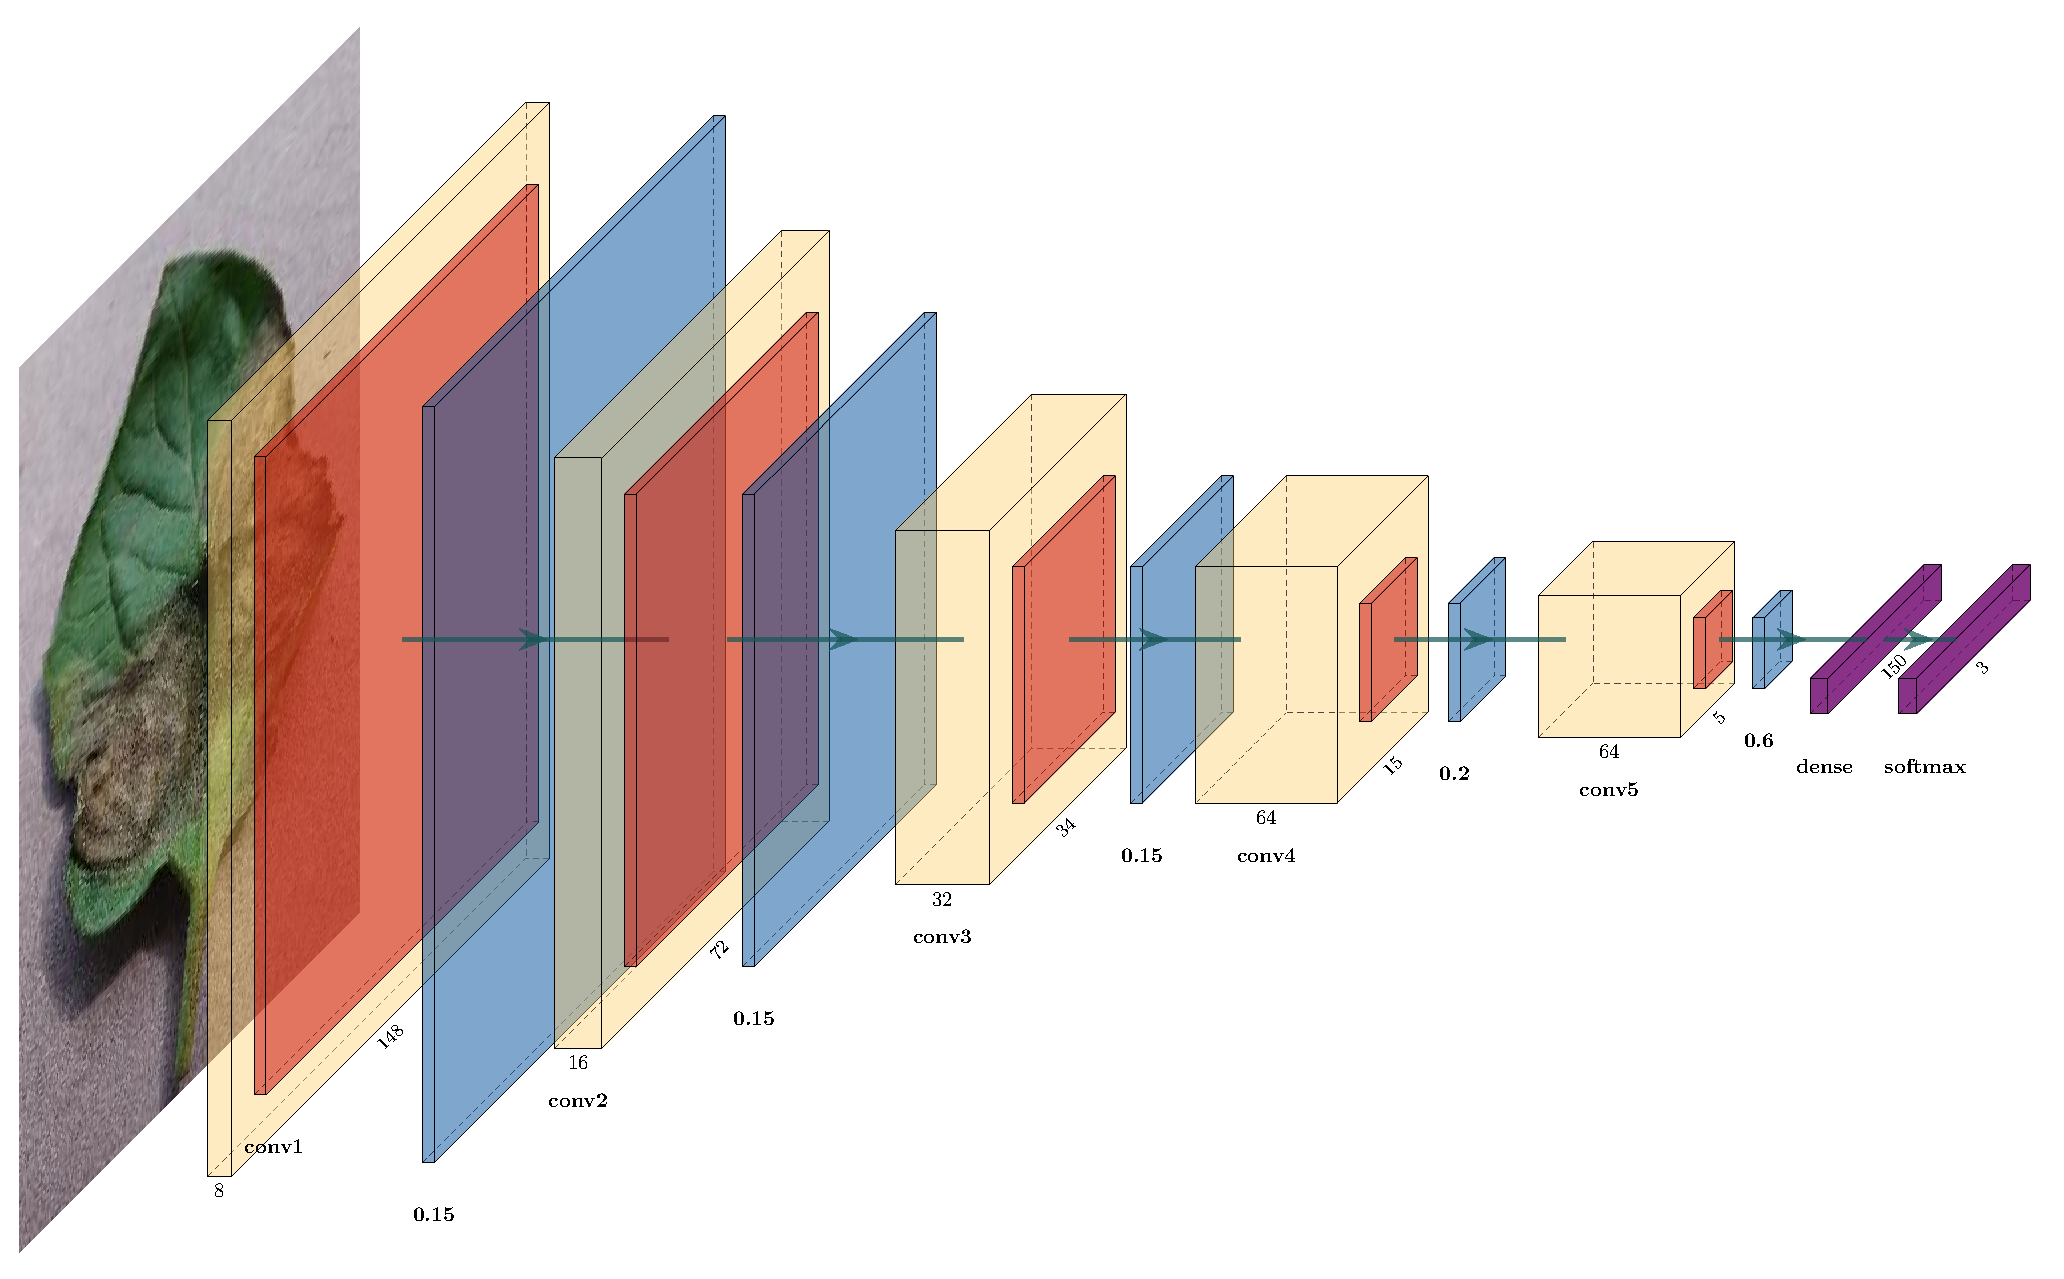
\includegraphics[width=\textwidth]{bilder/voter2.pdf}
	\caption{Veranschaulichung des zweiten Modells mit fünf Faltungs-, Pooling- und Dropout-Schichten (eigene Darstellung).}
	\label{voter2}
\end{figure}

Nun erhält die Architektur ihre letzte Kombination aus einer Faltungsschicht mit derselben Anzahl von Filtern und einer Max-Poolingschicht. Auch hier wird mit einer Dropout-Schicht, die die Rate von 60\% wie aus den Modellen \ref{sec:customNN} und \ref{model1_voter} bekannt ist, ergänzt. Letztendlich benötigt die Architektur des neuronalen Netzes noch zwei voll verbundene Schichten mit jeweils 150 und drei Knoten. Die erste voll verbundene Schicht verwendet die ReLU-Aktivierungsfunktion mit der L2-Regularisierung, die die Gewichte um den Faktor 0.002 berichtigt. Die letzte Schicht ist für die Klassifikation zuständig. Daher hat diese die Softmax-Aktivierungsfunktion.


~\newline
\paragraph{Training}
~\newline



Mit 100 Epochen wurde das Training dieses Modells gestartet. Des Weiteren wurde das Training so konfiguriert, dass nach 15 Epochen das Lernverfahren abgebrochen wird, wenn sich die minimale Kosten nicht verringern. Der Abbruch erfolgt bei der 92. Epoche, da die Kosten nicht kleiner werden. Das beste Modell bezüglich der minimalen Kosten wurde in der 77. Epoche gefunden und legt eine Genauigkeit auf dem Trainingsdatensatz von 96.54\% dar. 


~\newline
\subsection{Modell 3}
\label{model3_voter}
%\subsubsection{Struktur}

Ein weiteres Modell verwendet dieselbe Strategie des Modells \ref{model2_voter}. Hier wird auch auf viele Faltungsschichten gesetzt. Nach jeder Faltungsschicht mit der Max-Poolingschichtkomponente folgt eine Dropout-Schicht. Die erste Faltungsschicht nimmt wie bei allen anderen Modellen das Eingangsbild an und hat genau acht Filter. Anschließend folgt schon die erste Dropout-Schicht, die auf 15\% eingestellt ist. Nach diesem Muster wird die Architektur des neuronalen Netzes erstellt. Dies wird noch zwei mal wiederholt. Dabei verdoppelt sich iterativ die Anzahl der Filter in der Faltungsschicht. Des Weiteren sind bis dahin alle Dropout-Schichten auf den Wert 0.15 eingestellt. Die vierte Faltungsschicht hat genau so viele Filter wie die vorherige Faltungsschicht, nämlich 32. Daraufhin schließt sich die letzte Dropout-Schicht an, welche auf 60\% konfiguriert ist. Abschließend vervollständigt sich das Modell mit zwei voll verbundenen Schichten. Die erste folgende Schicht hat 150 Knoten mit der ReLU-Aktivierungsfunktion sowie L2-Regularisierung, die aus den anderen Modellen bekannt sind. Die letzte voll verbundene Schicht hat drei Knoten für die Klassifikation, die mittels der Softmax-Aktivierungsfunktion erfolgt.

\begin{figure}[h!]
	\centering
	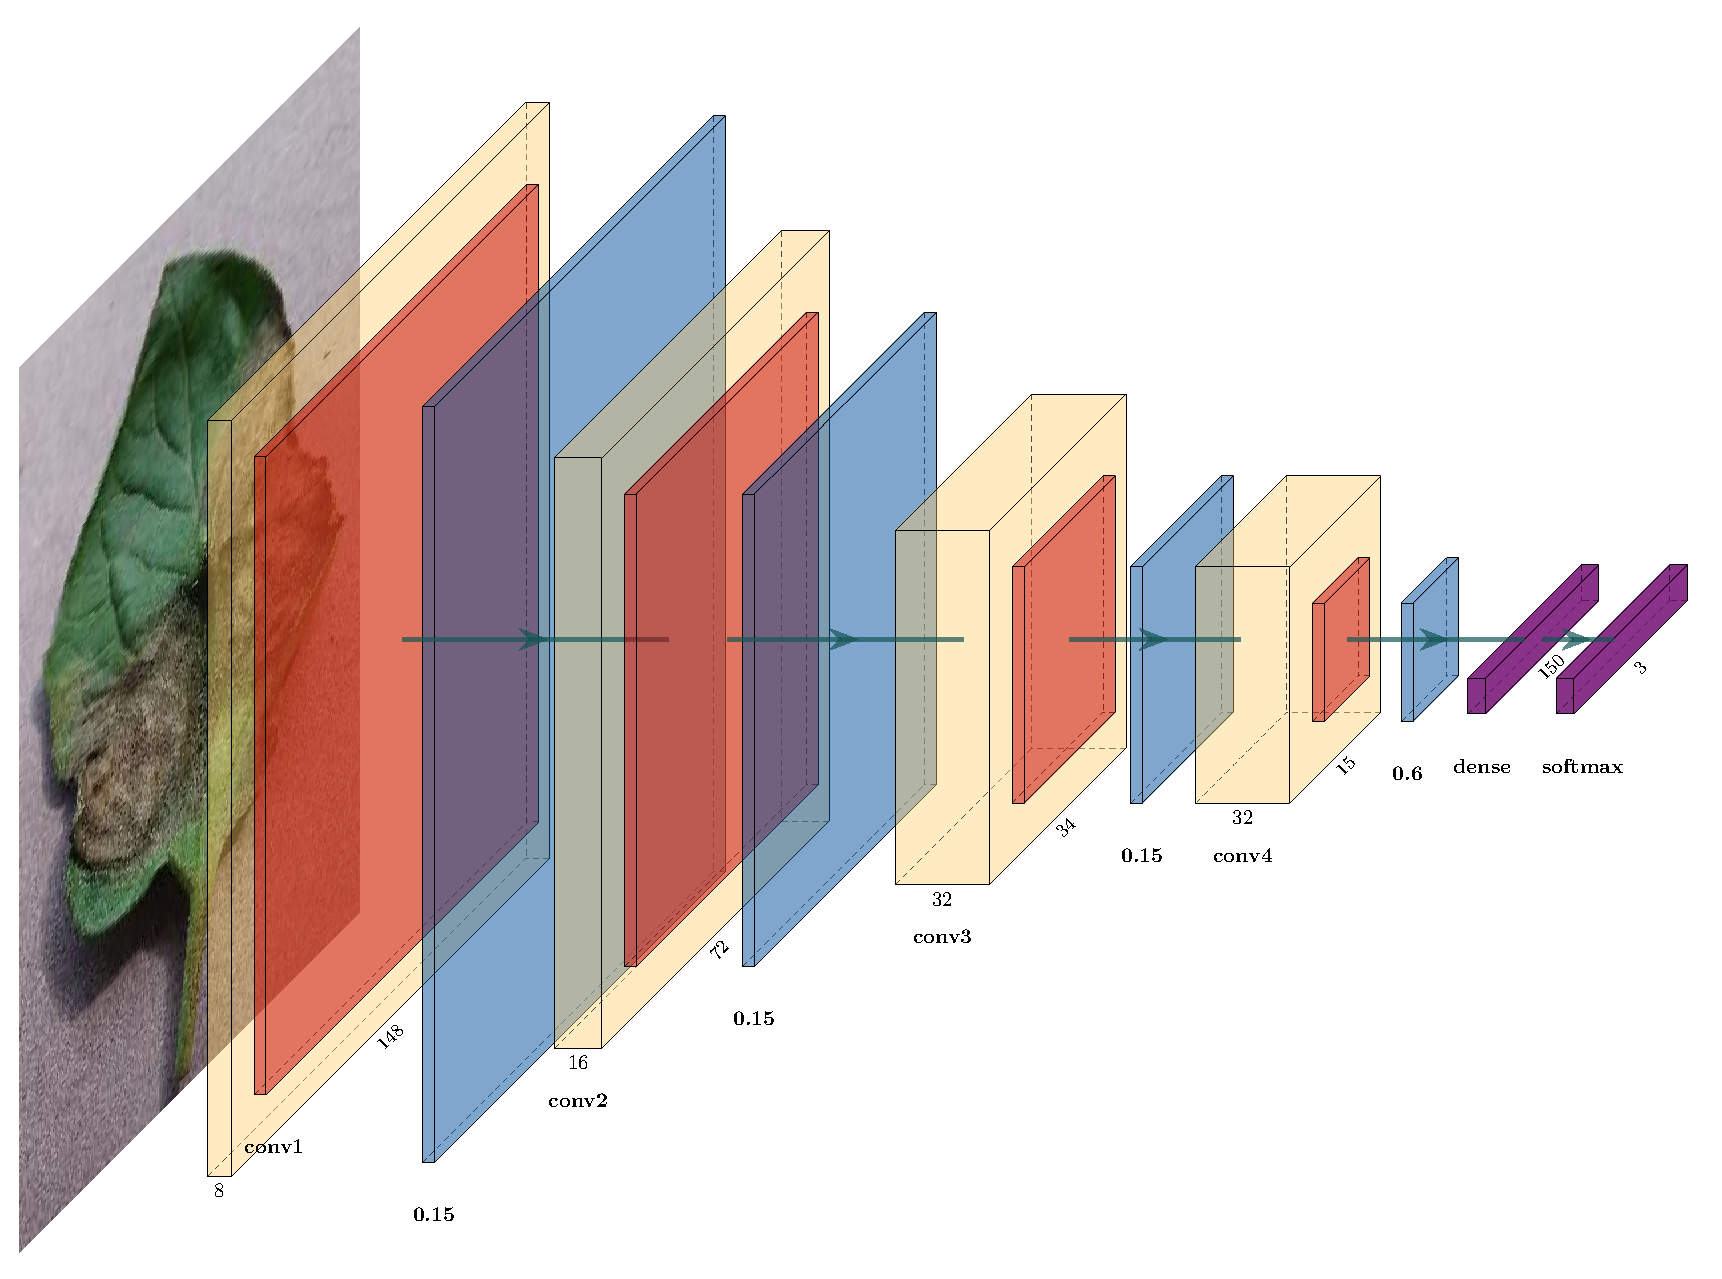
\includegraphics[width=\textwidth]{bilder/voter3.pdf}
	\caption{Veranschaulichung des dritten Modells mit vier Faltungs-, Pooling- und Dropout-Schichten (eigene Darstellung).}
	\label{voter3}
\end{figure}




\newpage
\paragraph{Training}
~\newline


Das Training des Modells wird auch hier mit 100 Epochen gestartet. Das Training wird abgebrochen, wenn nach 15 Epochen keine Verbesserung der Minimierung auftritt. Dies tritt bei der 79. Epoche ein. Das beste Modell bezüglich der minimalen Kosten wurde in der 64. Epoche entdeckt und die Genauigkeit liegt bei 96.92\%. 


\section{Transfer gelerntes Modell}
\label{sec:transferlearning}


Die Basisstruktur des folgenden neuronalen Netzes basiert auf der Grundlage des Lernens durch den Transfer von vortrainierten Modellen (engl. transfer learning). Die Idee dahinter ist, dass trainierte Modelle auf ein neues, aber verwandtes Problem angewendet werden. Solche Modelle werden in der Regel auf einem sehr großen Datensatz trainiert. Die gelernten einfachen Merkmale, zum Beispiel Formen und Figuren, werden wiederverwendet, um solche Repräsentationen nicht noch einmal trainieren zu müssen \cite{Subramanian2018,natural,Vasilev2019}. 



Da alle größeren vortrainierten Modelle keine Blattkrankheiten als Klassen haben, wird ein beliebiges, vortrainiertes Modell, hier VGG19\cite{VGG16}, verwendet. 

\begin{wrapfigure}{r}{5cm}
	\centering
	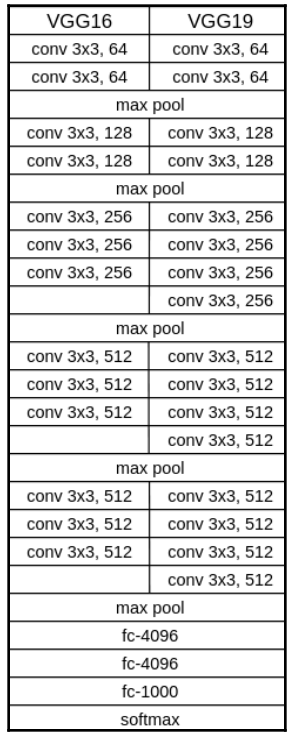
\includegraphics[width=0.18\textheight]{bilder/vgg19.PNG}
	\caption{Darstellung der VGG16 und VGG19 Struktur\cite{Vasilev2019}.}
	\label{VGG19_arch}
\end{wrapfigure}

Das neuronale Netzwerk besteht aus mehreren Blöcken, die mit zwei oder vier gestapelten Faltungsschichten in Kombination mit einer Max-Poolingschicht versehen sind. In Abbildung \ref{VGG19_arch} ist die Struktur der Architektur mit 16 und 19 Schichten visualisiert. Das Netzwerk hat bei zunehmender Tiefe deutlich mehr Filter in den Faltungsschichten. Die Anzahl der Filter reicht von 64 bis 512. Jede Faltungsschicht hat innerhalb eines Blocks dieselbe Anzahl von Filtern. Anschließend folgen drei voll verbundene Schichten. Davon sind zwei Schichten mit 4096 Knoten versehen. Die dritte Schicht hat 1000 Knoten\cite{Vasilev2019}. 


Um das vortrainierte Modell verwenden zu können, muss die letzte voll verbundene Schicht mit der Softmax-Aktivierungsfunktion entfernt werden. Nach der Entfernung werden zwei voll verbundene Schichten mit 150 und fünf Knoten hinzugefügt für die Klassifikation von fünf Klassen. Wichtig ist es zu beachten, dass die Gewichte des ursprünglichen VGG19-Modells eingefroren werden, um die extrahierten Merkmale aus dem großen Datensatz beibezuhalten. 


\paragraph{Training}
~\newline


Dieses Modell hat im Vergleich zu anderen Modellen die höchste Epochenanzahl, hier 150. Der Abbruch des Trainings erfolgt erst nach 35 Epochen bei einer Nicht-Verbesserung der minimalen Kosten. Dies geschieht bei diesem Modell ab der 103. Epoche. Die Genauigkeit des Modells beträgt 71.1\%. 




% kapitel2.tex
\chapter{Ergebnisse und Evaluierung}
\label{chapter:evaluation}

Hier werden die Ergebnisse von den trainierten Modellen gezeigt und diskutiert. Alle Ergebnisse wurden mit der folgenden Hardware mit diesen Komponenten erstellt: Zwei $Intel^{\textregistered} Xeon^{\textregistered}$ CPU E5-2650 @ 2.20GHz Prozessoren mit 112 Gb Arbeitsspeicher. Außerdem besitzt die Hardware eine Grafikkarte vom Typ NVIDIA GeForce GTX 1080 mit 8Gb Speicher.



\section{Ergebnisse}

Mithilfe der Genauigkeit und der Verlustfunktion können Aussagen darüber getroffen werden, wie gut die Modelle trainiert wurden. In diesem Abschnitt wird die Frage mittels Grafiken geklärt, ob eine Überanpassung beziehungsweise Unteranpassung stattgefunden hat. Des Weiteren werden die Ergebnisse der Modelle, die auf den Tomatendatensatz angewendet wurden, gezeigt.

\subsection{Auswertung des 5-Klassen-Modells}

In der Abbildung \ref{eval_acc_loss_5} erreichen die beiden Graphen die 96. Epoche. Das Training wurde in 

\begin{figure}[h!]
	
	\hfill
	\subfigure{
		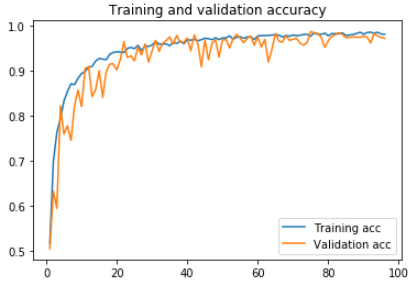
\includegraphics[width=0.44\textwidth]{model/final_model/final_model_acc.PNG}}
	\hfill
	\subfigure{
		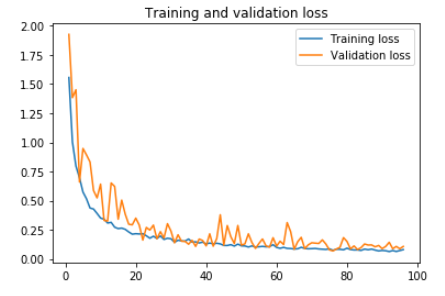
\includegraphics[width=0.48\textwidth]{model/final_model/final_model_loss.PNG}}
	\hfill
	\caption{Die linke Abbildung zeigt die Genauigkeit des Modells. Die andere Abbildung visualisiert die Werte von der Verlust-Funktion in der jeweiligen Epoche (eigene Darstellung).
	}
	\label{eval_acc_loss_5}
\end{figure}

\newpage
der 76. Epoche abgebrochen und hat eine Genauigkeit von 98.51\%. Da die beiden Graphen nah beieinander liegen, kann hier eine Über- und Unteranpassung ausgeschlossen werden. Des Weiteren stagnieren die Werte der Loss-Funktion auf dem Trainings- und Validationsdatensatz, so dass kein Anzeichen für eine Über- und Unteranpassung vorliegt.




In der Abbildung \ref{final_model_cm} ist klar zu erkennen, dass alle Krankheiten in über 98\% der Fälle korrekt klassifiziert wurden. Des Weiteren können alle Krankheiten ausgehend von einem gesunden Blatt unterschieden werden. Lediglich die Krautfäule (late blight) wurde genau einmal falsch als ein gesundes Blatt erkannt. Die Unterscheidung zwischen der Krautfäule (late blight) und Dürrfleckenkrankheit (early blight) kann in der Größenordnung von etwa fünf bis sechs Fehlklassifizierung liegen. Darüber hinaus weist das Modell zwei Fehlklassifizierungen zwischen der Samtfleckenkrankheit (leaf mold) und Dürrfleckenkrankheit (early blight) auf.

\begin{figure}[h!]
	\centering
	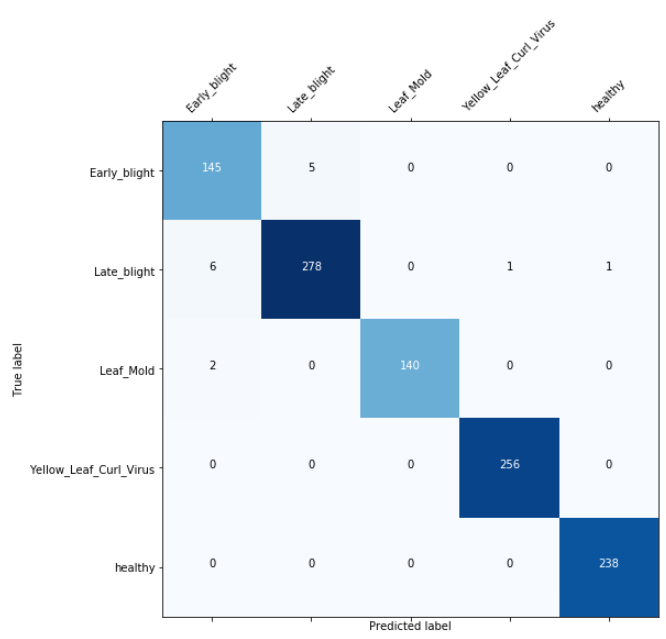
\includegraphics[width=0.83\textwidth]{model/final_model/final_model_cm.PNG}
	\caption{Veranschaulichung von Klassifizierungen des 5-Klassen Modells (eigene Darstellung).}
	\label{final_model_cm}
\end{figure}

\newpage
\subsection{Auswertung des Voters}

In diesem Unterabschnitt werden jeweils die Ergebnisse der Modelle, die für zwei Krankheiten trainiert wurden, diskutiert. Anschließend wird eine Wahrheitsmatrix gezeigt, die das Ergebnis der drei Modelle mithilfe des Voting-Verfahrens veranschaulicht. Die Performanz des Voters wird dann mit den einzelnen Modellen verglichen.


\subsubsection{Modell 1}

Die Abbildung \ref{eval_acc_loss_voter1} zeigt, dass die Genauigkeit und die Verluste unter großen Schwankungen stehen. Der Verlauf des Validationsdatensatzes weist eine alternierende Struktur auf. Das Training wurde in der 35. Epoche abgebrochen, da die Werte zu dieser Epoche auf der selben Höhe liegen und keine weiteren Verbesserungen auftraten. Dort befindet sich auch der minimalste Verlust. Die Werte der Loss-Funktion werden mit steigender Epochenanzahl nicht kleiner. Letztendlich besitzt das Modell eine Genauigkeit von 97.94\%. Des Weiteren ist hier eine Überanpassung erkennbar, weil der Verlauf des Validationsdatensatzes in der rechten Abbildung oberhalb des Trainingsverlaufs ist.


\begin{figure}[h!]
	
	\hfill
	\subfigure{
		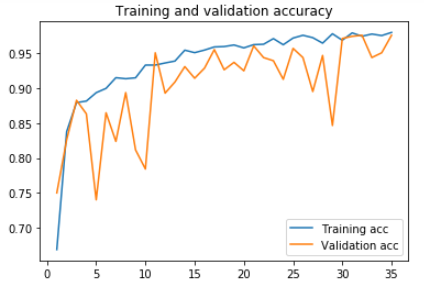
\includegraphics[width=0.48\textwidth]{model/voter1/voter1_acc.PNG}}
	\hfill
	\subfigure{
		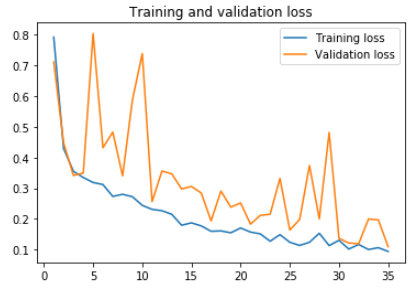
\includegraphics[width=0.47\textwidth]{model/voter1/voter1_loss.PNG}}
	\hfill
	\caption{Die Genauigkeit des ersten Modells ist in der linken Abbildung visualisiert. Die Verläufe der beiden Datensätze liegen nah beieinander. Die Werte der Verlust-Funktion von dem Validationsdatensatz nähern sich mit steigender Epochenanzahl an den Trainingsdatensatz an. Dies wird in der rechten Abbildung gezeigt (eigene Darstellung).
	}
	\label{eval_acc_loss_voter1}
\end{figure}

In Abbildung \ref{voter1_cm} wird eine Matrix veranschaulicht, die die Performance der Klassifizierung darstellt. Gesunde Blätter werden in diesem Modell stets richtig klassifiziert. Ausgehend von der Krautfäule existieren zwei Fehlklassifizierung. Diese werden als Dürrfleckenkrankheit (early blight) wahrgenommen. Blätter von der Dürrfleckenkrankheit werden vier Mal als Krautfäule erkannt.

\begin{figure}[h!]
	\centering
	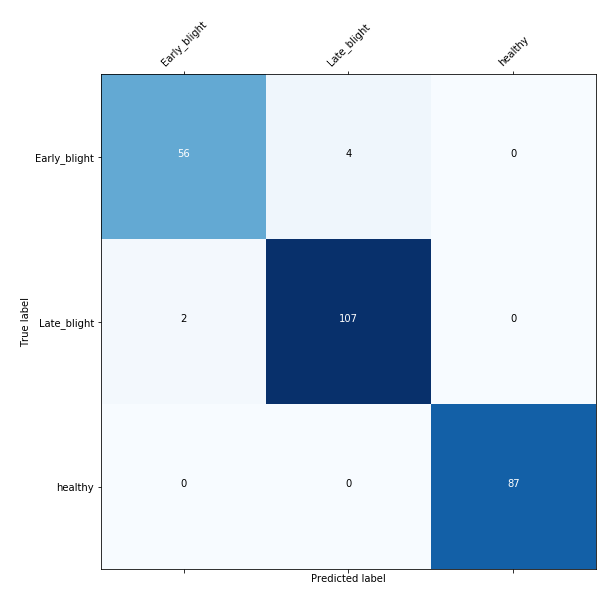
\includegraphics[width=0.8\textwidth]{model/voter1/voter1_cm.PNG}
	\caption{Veranschaulichung von Klassifizierungen des ersten Voter-Modells (eigene Darstellung).}
	\label{voter1_cm}
\end{figure}

\newpage
\subsubsection{Modell 2}

Auch das zweite Modell hat eine leichte Überanpassung. In der Abbildung \ref{eval_acc_loss_voter2} sind die Graphen bezüglich der Genauigkeit und der Verlustwerte abgebildet. In beiden Graphen

\begin{figure}[h!]
	
	\hfill
	\subfigure{
		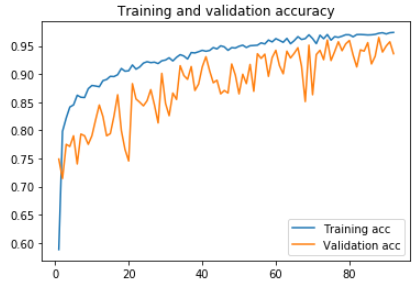
\includegraphics[width=0.48\textwidth]{model/voter2/voter2_acc.PNG}}
	\hfill
	\subfigure{
		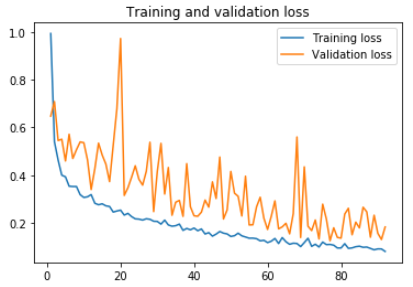
\includegraphics[width=0.48\textwidth]{model/voter2/voter2_loss.PNG}}
	\hfill
	\caption{Die linke Abbildung veranschaulicht die Genauigkeit des Modells in den jeweiligen Datensatz. Die Verlust-Werte (rechte Abbildung) liegen nicht eng beieinander (eigene Darstellung).
	}
	\label{eval_acc_loss_voter2}
\end{figure}

ist diese Überanpassung erkennbar. In der linken Abbildung ist der Verlauf des Trainingsdatensatzes oberhalb des Validationsdatensatzes. In dem rechten Graphen befindet sich der Verlauf des Validationsdatensatzes oberhalb des Trainingsdatensatzes. Außerdem weist auch hier der Validationsdatensatz einen alternierenden Verlauf an. Die beiden Graphen gehen bis zur 92. Epoche, da das Training früher abgebrochen wurde. Der minimalste Verlust wurde in der 77. Epoche gefunden und hat in dieser Epoche eine Genauigkeit von 96.54\%. Dieses Modell zu dieser Epoche legt die besten Ergebnisse vor.



Die Abbildung \ref{voter2_cm} veranschaulicht, dass alle gesunden Blätter korrekt erkannt sowie nicht als Krankheit verwechselt werden. Solche Ergebnisse zeigt auch die Dürrfleckenkrankheit (early blight). Lediglich erkennt das Modell zweimal die Krankheit Krautfäule (late blight) als Dürrfleckenkrankheit (early blight).


\begin{figure}[h!]
	\centering
	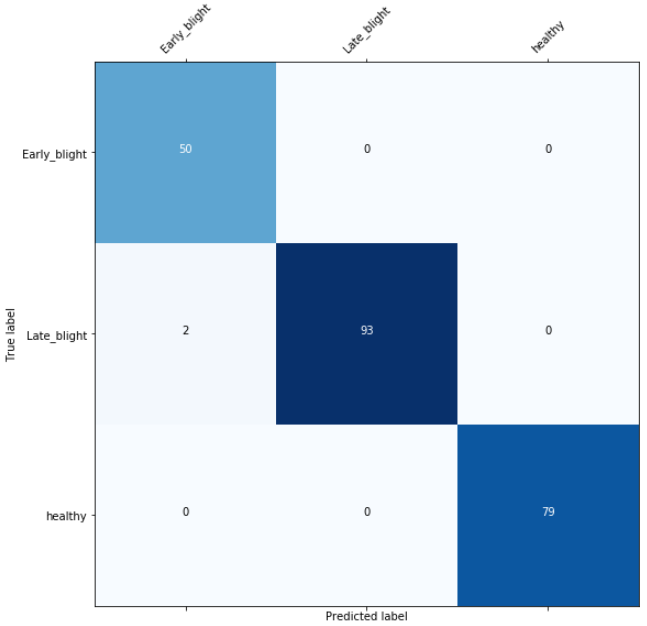
\includegraphics[width=0.83\textwidth]{model/voter2/voter2_cm.PNG}
	\caption{Veranschaulichung von Klassifizierungen des zweiten Voter-Modells (eigene Darstellung).}
	\label{voter2_cm}
\end{figure}


\subsubsection{Modell 3}

In der Abbildung \ref{eval_acc_loss_voter3} werden die beiden Graphen bezüglich der Genauigkeit und der Verluste bis zur 79. Epoche visualisiert. Die Genauigkeit und die Loss-Werte des Validationsdatensatzes verlaufen in den ersten 40 Epochen alternierend mit großem Abstand zu dem Trainingsdatensatz. Ab der 40. Epoche nähern sich die beiden Datensätze an.

\begin{figure}[h!]
	
	\hfill
	\subfigure{
		\includegraphics[width=0.48\textwidth]{model/voter3/voter3_acc.PNG}}
	\hfill
	\subfigure{
		\includegraphics[width=0.48\textwidth]{model/voter3/voter3_loss.PNG}}
	\hfill
	\caption{Die linke Abbildung zeigt, dass sich die Genauigkeit des Modells auf dem Validationsdatensatz mit steigender Epochenanzahl an den Trainingsdatensatz annähert. Die Verlust-Funktion zeigt das selbe Verhalten in der rechten Abbildung (eigene Darstellung).
	}
	\label{eval_acc_loss_voter3}
\end{figure}

Dieser Effekt ist bei den beiden Grafiken zu sehen. In der 64. Epoche, in der das

\begin{figure}[h!]
	\centering
	\includegraphics[width=0.75\textwidth]{model/voter3/voter3_cm.PNG}
	\caption{Veranschaulichung von Klassifizierungen des dritten Voter-Modells (eigene Darstellung).}
	\label{voter3_cm}
\end{figure}
~\newline
Training abgebrochen wurde, hat das dritte Modell die höchste Genauigkeit mit 96.62\%. Die Struktur der Graphen zeigen eine Stagnierung mit steigender Epochenanzahl.



Des Weiteren hat das Modell eine leichte Überanpassung. Die Genauigkeit liegt bei dem Trainingsdatensatz höher als der Validationsdatensatz. Weiterhin sind die Verlustwerte bei dem Trainingsdatensatz geringer als der Validationsdatensatz.

Die Abbildung \ref{voter3_cm} visualisiert die Ergebnisse der Klassifikation mit dem Testdatensatz. Es existiert keine Verwechslung mit gesunden Blättern. Des Weiteren werden diese auch alle korrekt als gesunde Blätter klassifiziert. Die Dürrfleckenkrankheit (early blight) wird genau einmal falsch als Krautfäule (late blight) erkannt. Mit sechs Fehlklassifizierungen zeigt die Klasse \glqq late blight\grqq, dass Fehlklassifizierungen mit der Dürrfleckenkrankheit (early blight) auftreten können.


\subsubsection{Wahrheitsmatrix mit den drei Modellen}

In der Abbildung \ref{voter_combined} zeigt sich, dass der Voter die Ergebnisse der einzelnen Modelle verbessern kann. Nur das zweite Modell weist ohne die Hilfe des Voters bessere Ergebnisse auf.

\begin{figure}[h!]
	\centering
	\includegraphics[width=0.73\textwidth]{bilder/voter.PNG}
	\caption{Veranschaulichung von Klassifizierungen mit drei Modellen, die mithilfe von einem Voting-Verfahren bestimmt wurden (eigene Darstellung).}
	\label{voter_combined}
\end{figure}


Das zweite Modell hat lediglich zwei Fehlklassifikation. Der Voter klassifiziert gegenüber dem ersten Modell deutlich besser die Dürrfleckenkrankheit (early blight). Allerdings ist die Erkennung der Krautfäule (late blight) mit dem ersten Modell minimal besser. Hier verringert sich die Anzahl der Fehlklassifizierung von drei auf zwei. Das dritte Modell hat bei der Erkennung der Krautfäule (late blight) sechs Fehlklassifizierungen. Der Voter erkennt hierbei nur drei Exemplare falsch.


\subsection{Auswertung des transfergelernten Modells}


Die Abbildung \ref{eval_acc_loss_transfer} zeigt den Verlauf des Trainings in dem Aspekt der Genauigkeit und der Verlust-Funktion. Dieser geht bis zu der 103. Epoche. Der geringste Verlustwert wurde in der 68. Epoche gefunden und das Modell besitzt eine Genauigkeit von 71.1\%. Die Graphen in den beiden Abbildungen liegen nicht eng beieinander. Des Weiteren ist dieses Modell das einzige Modell mit einer Unteranpassung. Die Unteranpassung lässt sich daran erkennen, dass die Genauigkeit des Trainingsdatensatzes unterhalb des Validationsdatensatzes liegt. Außerdem sind die Verlustwerte bei dem Validationsdatensatz geringer als bei dem Trainingsdatensatz.

\begin{figure}[h!]
	\hfill
	\subfigure{
		\includegraphics[width=0.48\textwidth]{model/transfer/acc.png}}
	\hfill
	\subfigure{
		\includegraphics[width=0.48\textwidth]{model/transfer/loss.png}}
	\hfill
	\caption{Genauigkeit (links) und Loss-Funktion (rechts) des transfergelernten Modells. In beiden Graphiken ist die Unteranpassung sichtbar (eigene Darstellung).
	}
	\label{eval_acc_loss_transfer}
\end{figure}



In der Abbildung \ref{transfer_confusion_matrix} sind die Schwächen des Modells klar zu erkennen. Größtenteils wird die Krankheit korrekt erkannt. Dennoch treten Fehlklassifizierungen auf. Bei der Klasse \glqq early blight\grqq~gibt es keine Verwechslung mit gesunden Blättern. Allerdings werden zwei Mal gesunde Blätter als die Dürrfleckenkrankheit (early blight) erkannt. Des Weiteren hat diese Klasse leichte Schwierigkeiten mit der Klasse \glqq late blight\grqq. Die Anzahl der Fehlklassifikation liegt bei neun. Die restlichen zwei Klassen haben maximal fünf Fehlklassifikationen.

Die Klasse \glqq late blight\grqq~ hat Schwierigkeiten mit den Klassen \glqq early blight\grqq~und \glqq leaf mold\grqq. Mit 18 beziehungsweise 10 Fehlerkennung ist die Fehlerrate recht hoch. Am wenigsten hat die Klasse Probleme mit der Krankheit \glqq TYLCV\grqq.

Die beste Performance bezüglich der Klassifikation hat die Klasse \glqq leaf mold\grqq. Diese hat höchstens zwei Fehlklassifkationen in allen Klassen. Die schlechtesten Ergebnisse sind von der Klasse \glqq TYLCV\grqq. Diese zeichnet sich durch eine hohe Fehlerkennung mit der Dürrfleckenkrankheit (early blight), nämlich 26, aus.
Auch bei dem Vergleich mit den anderen Klassen schneidet die Klasse \glqq TYLCV\grqq deutlich schlechter ab. Nur die Erkennung von gesunden Blättern schlägt genau drei Mal fehl. Die Klasse der gesunden Blätter hat mit fünf Fehlerkennungen bei der Klasse \glqq leaf mold\grqq~ leichte Defizite.

\begin{figure}[h!]
	\centering
	\includegraphics[width=0.83\textwidth]{model/transfer/confusion_matrix.PNG}
	\caption{Veranschaulichung von Klassifizierungen des Modells, welches durch Transfer Learning gelernt hat (eigene Darstellung).}
	\label{transfer_confusion_matrix}
\end{figure}


\section{Evaluierung}

Manche Blattkrankheiten, zum Beispiel die Dürrfleckenkrankheit und die Krautfäule, treten nicht nur bei Tomaten auf. Andere Nachtschattengewächse beispielsweise Kartoffeln sind auch von diesen Krankheiten betroffen. In diesem Abschnitt werden diese Krankheiten auf den Blättern von Kartoffeln mit den Modellen, die eigentlich für Tomaten vorgesehen sind, vorhergesagt. In Abbildung \ref{potatoes_combined} ist eindeutig zu sehen, dass die trainierten Modelle auf dem Kartoffeldatensatz keine gute Ergebnisse zeigen. Die Dürrfleckenkrankheit (early blight) wird am häufigsten bei allen Modellen als gesunde Blätter erkannt. Die Krautfäule (late blight) wird auch sehr häufig als gesunde Blätter klassifiziert. Des Weiteren ist die 


\begin{figure}[h!]
	\centering
	\includegraphics[width=\textwidth]{potatoes_plots/combined.PNG}
	\caption{Veranschaulichung von Klassifizierungen des Modells auf dem Kartoffeldatensatz (eigene Darstellung).}
	\label{potatoes_combined}
\end{figure}

Erkennung von Krautfäule bei allen Modellen kaum vorhanden. In dem ersten Modell wurde die Krautfäule lediglich drei Mal erkannt. In dem dritten Modell wurde diese Krankheit höchstens 19 Mal klassifiziert. Nur in dem ersten Modell werden gesunde Blätter überproportional als gesunde Blätter erkannt. Andere Modelle haben mit der Erkennung der gesunden Blätter Schwierigkeiten und erkennen gesunde Blätter oft als Dürrfleckenkrankheit (early blight). Der Voter sorgt für keine Besserung und zeigt das Verhalten wie die anderen Modelle. Eine mögliche Erklärung für diese Ergebnisse können die unterschiedliche Struktur der Blattoberfläche sowie die Form sein. Die Modelle haben nicht nur die Erkennung der Flecken gelernt, sondern auch die Struktur von dem vorliegenden Blatt.

In den Abbildungen \ref{eval_pot_early} und \ref{eval_pot_late} ist klar zu sehen, dass die Aderung des Blattes beispielsweise unterschiedlich ist. Weiterhin ähneln die Blätter von Tomaten einer Pfeilspitze. Bei Kartoffeln ist die Form eher oval.


\begin{figure}[t!]
	\hfill
	\subfigure{
		\includegraphics[width=0.43\textwidth]{potatoes_plots/tom_early.JPG}}
	\hfill
	\subfigure{
		\includegraphics[width=0.43\textwidth]{potatoes_plots/pot_early.JPG}}
	\hfill
	\caption{Visualisierung der Dürrfleckenkrankheit bei Tomaten (links) und Kartoffeln (rechts) (eigene Darstellung).
	}
	\label{eval_pot_early}
\end{figure}

\begin{figure}[h!]
	\hfill
	\subfigure{
		\includegraphics[width=0.43\textwidth]{potatoes_plots/tom_late.JPG}}
	\hfill
	\subfigure{
		\includegraphics[width=0.43\textwidth]{potatoes_plots/pot_late.JPG}}
	\hfill
	\caption{Visualisierung der Krautfäule bei Tomaten (links) und Kartoffeln (rechts) (eigene Darstellung).
	}
	\label{eval_pot_late}
\end{figure}















\newpage
\section{Visualisierung}

Die Klassenentscheidung von neuronalen Netzen ist auf den ersten Blick nicht ganz klar, weil grundsätzliche Visualisierungen den Benutzern nicht angezeigt werden. Dadurch entsteht der Eindruck, dass neuronale Netze wie eine Blackbox wirken. Durch Visualisierungen können die Entscheidungen von neuronalen Netzen nachvollziehbar dargestellt werden. In diesem Abschnitt werden die Aktivierungswerte in den Faltungschichten visualisiert. Des Weiteren können die Aktivierungswerte in einer Heatmap dargestellt werden. Alle Abbildungen von jeder Krankheit und gesunden Blättern werden im Anhang A-E auf den Seiten \pageref{anahnga} - \pageref{anahngd} bereitgestellt.


\begin{figure}[h!]
	\hfill
	\subfigure{
		\includegraphics[width=0.44\textwidth]{visualisierungen/healthy/heatmap_ohne/cropped_ohne.png}}
	\hfill
	\subfigure{
		\includegraphics[width=0.43\textwidth]{visualisierungen/healthy/heatmap_mit/cropped_mit.png}}
	\hfill
	\caption{Die linke Darstellung hat keine Normierung der Farbwerte. Das rechte Bild mit der Normierung zeigt schwache Aktivierungswerte deutlicher an (eigene Darstellung).
	}
	\label{vis_normalised_rgb}
\end{figure}


Angemerkt sei, dass die Darstellung mit normierten Farbwerte visualisiert wird. Die Abbildung \ref{vis_normalised_rgb} zeigt deutlich, dass die Aktivierungswerte in der normierten Grafik (rechts) erkennbarer als die nicht normierten Bilder sind. Das linke Bild zeigt zwar das Hintergrundbild, allerdings sind schwache Aktivierungswerte kaum erkennbar.

\subsection{Gesunde Blätter}

Die Abbildung \ref{healthy_sample} wird als Ausgangsbild für die Visualisierung benutzt. Die dritte Faltungschicht ist für dieses Beispiel ideal, da die Visualisierung noch Strukturen des Blattes aufweist (s. Abbildung \ref{healthy6}). 
\begin{figure}[h!]
	\centering
	\includegraphics[width=0.5\textwidth]{visualisierungen/healthy/healthy_sample.jpg}
	\caption{Das Beispielbild für die Visualisierung von gesunden Blättern (eigene Darstellung).}
	\label{healthy_sample}
\end{figure}

\newpage
Die Aderung und die Umrandung des Blattes ist noch in der Abbildung erkennbar. Außerdem hat das 5-Klassen Modell nur vereinzelt den Hintergrund gelernt. Insgesamt haben 51 Filter auf das Eingangsbild nicht reagiert. Die vierte und fünfte Faltungschicht, die sich in dem Anhang befinden, zeigen abstrakte kleine Konstrukte, die nicht genau zuordenbar sind.

\begin{figure}[h!]
	\centering
	\includegraphics[width=\textwidth]{visualisierungen/healthy/activation/healthy6.JPG}
	\caption{Visualisierung der Aktivierungswerte in der dritten Faltungschicht von gesunden Blättern (eigene Darstellung).}
	\label{healthy6}
\end{figure}

In der Heatmap \ref{conv2d_8_healthy} ist klar zu sehen, dass zwei Filter den Hintergrund gelernt haben. Außerdem sind die Konzentrationen großteils an dem Rand des Blattes angesiedelt und treten vereinzelt auf. In der letzten Faltungschicht sind die Konzentrationen signifikant größer und mittig positioniert (s. Abbildung \ref{conv2d_10_heat}).

\begin{figure}[h!]
	\centering
	\includegraphics[width=\textwidth]{visualisierungen/healthy/heatmap_mit/conv2d_8.png}
	\caption{Visualisierung der Aktivierungswerte als Heatmap in der dritten Faltungschicht von gesunden Blättern (eigene Darstellung).}
	\label{conv2d_8_healthy}
\end{figure}

\newpage
\subsection{Dürrfleckenkrankheit}

Die erste Krankheit, die hier visualisiert wird, ist die Dürrfleckenkrankheit. Die Abbildung \ref{early_visual} zeigt das Ausgangsbild. Das Blatt hat vermehrt Flecken auf der rechten Seite. Diese verlaufen an der Hauptaderung des Blattes entlang. In der unteren linken Ecke befinden sich vereinzelte Flecken, die sowohl an der Hauptaderung als auch an dem Rand des Blattes liegen. Des Weiteren weist das Bild gelbe Bereiche in dem unteren rechten Bereich auf.


%\begin{figure}[h!]
%	\centering
%	\includegraphics[width=0.45\textwidth]{visualisierungen/early/early.jpg}
%	\caption{Das Beispielbild für die Visualisierung der Dürrfleckenkrankheit (eigene Darstellung).}
%	\label{early_visual}
%\end{figure}

\begin{wrapfigure}{r}{8cm}
	\centering
	\includegraphics[width=0.45\textwidth]{visualisierungen/early/early.jpg}%
	\caption{Das Beispielbild für die Visualisierung der Dürrfleckenkrankheit (eigene Darstellung).}
	\label{early_visual}
\end{wrapfigure}

In der dritten Faltungschicht (s. Abbildung \ref{early_visual_act}) hat das Modell einige Male den Hintergrund gelernt. Großteil der Aktivierungen finden in der rechten Hälfte an der Hauptaderung statt. Das Modell ist auch in der Lage, gelbe Flächen auf der rechten Seiten zu lernen. Weiterhin sind die Flecken auf der unteren linken Seite vereinzelt in der Abbildung erkennbar. 45 Filter haben in dieser Faltungschicht nicht auf das Bild angesprochen. Die vierte Faltungschicht in der Abbildung \ref{early8_anhang} zeigt dasselbe Verhalten wie in der dritten Schicht. Allerdings ist in der vierten Schicht die Reaktion deutlich erkennbarer.

\begin{figure}[h!]
	\centering
	\includegraphics[width=\textwidth]{visualisierungen/early/activation/early6.JPG}
	\caption{Visualisierung der Aktivierungswerte in der dritten Faltungschicht von der Dürrfleckenkrankheit (eigene Darstellung).}
	\label{early_visual_act}
\end{figure}

Die Aktivierungswerte konzentrieren sich an Stellen, an denen die Flecken vorhanden sind (s. Abbildung \ref{conv2d_8_heat_early}). Dabei wird nicht nur die rechte Seite erkannt, sondern auch die Flecken an der unten linken Ecke. Des Weiteren lernt die nachfolgende Schicht (s. Abbildung \ref{conv2d_9_anhang}) den Hintergrund nicht mehr.

\begin{figure}[h!]
	\centering
	\includegraphics[width=\textwidth]{visualisierungen/early/heatmap_mit/conv2d_8.png}
	\caption{Visualisierung der Aktivierungswerte als Heatmap in der dritten Faltungschicht von der Dürrfleckenkrankheit (eigene Darstellung).}
	\label{conv2d_8_heat_early}
\end{figure}





\newpage
\subsection{Tomato Yellow Leaf Curl Virus}

Das TYLCV-Virus zeichnet sich durch die Krümmung der Blattränder sowie die Gelbfärbung des Blattes aus. Die Abbildung \ref{yellow_sample} veranschaulicht deutlich die Symptome der Viruserkrankung. Die beiden Seitenränder sind gekrümmt und in gelb verfärbt. Außerhalb der Blattränder sind manche Regionen des Blattes von der Färbung betroffen.

%\begin{figure}[h!]
%	\centering
%	\includegraphics[width=0.5\textwidth]{visualisierungen/yellow/yellow_sample.jpg}
%	\caption{Das Beispielbild für die Visualisierung des TYLCV-Virus (eigene Darstellung).}
%	\label{yellow_sample}
%\end{figure}

\begin{wrapfigure}{r}{8cm}
	\centering
	\includegraphics[width=0.45\textwidth]{visualisierungen/yellow/yellow_sample.jpg}%
	\caption{Das Beispielbild für die Visualisierung des TYLCV-Virus (eigene Darstellung).}
	\label{yellow_sample}
\end{wrapfigure}


Das Bild \ref{yellow6_act_vis} zeigt deutlich, dass die Ränder des Blattes für das Modell ein Merkmal für die Krankheit darstellt. Das Modell hat jeweils eine Seite des Randes gelernt. Einige Filter in der dritten Faltungschicht sind in der Lage, beide Seiten als Merkmale zu erkennen. Die gelben Verfärbungen, die sich außerhalb des Blattrandes befinden, werden von wenigen Filter erkannt. Des Weiteren fasst das Modell den Hintergrund des Bildes noch als Merkmal auf. Die nachfolgende Schicht hat dieses Problem nicht (s. Abbildung \ref{yellow8_anhang}). Weiterhin hat das Modell in der dritten Faltungschicht 62 inaktive Filter.

\begin{figure}[h!]
	\centering
	\includegraphics[width=\textwidth]{visualisierungen/yellow/activation/yellow6.JPG}
	\caption{Visualisierung der Aktivierungswerte in der dritten Faltungschicht von dem TYLCV-Virus (eigene Darstellung).}
	\label{yellow6_act_vis}
\end{figure}

Die Heatmap (s. Abbildung \ref{yellow_heat_vis}) bestätigt, dass sich die Aktivierungen auf die Ränder des Blattes konzentrieren. In der ersten Zeile und der fünften Spalte ist ein Filter zu sehen, welcher hauptsächlich nur auf die Verfärbung außerhalb des Randes reagiert.

\begin{figure}[h!]
	\centering
	\includegraphics[width=\textwidth]{visualisierungen/yellow/heapmap_mit/conv2d_8.png}
	\caption{Visualisierung der Aktivierungswerte als Heatmap in der dritten Faltungschicht von dem TYLCV-Virus (eigene Darstellung).}
	\label{yellow_heat_vis}
\end{figure}



\newpage
\subsection{Samtfleckenkrankheit}

\begin{wrapfigure}{r}{7cm}
	\centering
	\includegraphics[width=0.45\textwidth]{visualisierungen/leaf_mold/mold_sample.jpg}%
	\caption{Das Beispielbild für die Visualisierung der Samtfleckenkrankheit (eigene Darstellung).}
	\label{mold_sample}
\end{wrapfigure}


In der Abbildung \ref{mold_sample} ist ein Blatt mit der Samtfleckenkrankheit abgebildet. Sehr viele gelbe Flecken sind in der Spitze des Blattes konzentriert. Im Inneren des Blattes auf der mittleren Höhe sind einige Ausprägungen sichtbar. Das Modell reagiert jeweils auf den linken und rechten Rand des Blattes. Die Abbildung \ref{mold6_act_vis} präsentiert deutlich, dass in der dritten Faltungschicht die Ausprägungen in der oberen Spitze nur von wenigen Filter angesprochen werden. In der vierten Faltungschicht (s. Abbildung \ref{mold8_anhang}) ist es zu abstrakt, um zu erkennen, ob das Modell das Verhalten der vorherigen Schicht übernommen hat. Des Weiteren zeigen in der dritten Faltungschicht 47 Filter keine Reaktion auf das Eingangsbild.

\begin{figure}[h!]
	\centering
	\includegraphics[width=\textwidth]{visualisierungen/leaf_mold/activation/mold6.JPG}
	\caption{Visualisierung der Aktivierungswerte in der dritten Faltungschicht von der Samtfleckenkrankheit (eigene Darstellung).}
	\label{mold6_act_vis}
\end{figure}
~\newline
Ein interessantes Merkmal, welches in den Aktivierungswerten nicht zu sehen ist, ist der horizontale Verlauf ausgehend von der Hauptaderung. Einige Filter in der Abbildung \ref{mold6_heat_vis} reagieren sehr stark darauf, zum Beispiel der Filter in der ersten Spalte und der sechsten Zeile. Des Weiteren sind die Ränder und die vorhin beschriebenen Positionen der Flecken relevant für das Modell. Dennoch lernt das Modell einige Male den Hintergrund.

\begin{figure}[h!]
	\centering
	\includegraphics[width=\textwidth]{visualisierungen/leaf_mold/heatmap_mit/conv2d_8.png}
	\caption{Visualisierung der Aktivierungswerte als Heatmap in der dritten Faltungschicht von der Samtfleckenkrankheit (eigene Darstellung).}
	\label{mold6_heat_vis}
\end{figure}



\newpage
\subsection{Krautfäule}

\begin{wrapfigure}{r}{7cm}
	\centering
	\includegraphics[width=0.45\textwidth]{visualisierungen/late/late_sample.jpg}%
	\caption{Das Beispielbild für die Visualisierung der Krautfäule (eigene Darstellung).}
	\label{late_sample}
\end{wrapfigure}


Das Beispielbild \ref{late_sample} veranschaulicht die typischen Ausprägungen von der Krautfäule. Diese zeichnen sich durch große braune Flecken aus. Um diese treten hellgrüne Verfärbungen auf, die das Blatt blass wirken lassen. Außerdem gibt es keine bevorzugte Position, auf der Ausprägungen auftreten. In der dritten Faltungschicht (s. Abbildung \ref{late6_act_vis}) ist zu erkennen, dass die Krümmung des linken Rands von dem Modell als interessantes Merkmal angesehen wird. Sehr viele Filter reagieren auf dieses Merkmal. Auch die Blattoberfläche ist für das Modell interessant. In der zehnten Spalte und der vierten Zeile sowie der sechsten Spalte und der ersten Zeile sind zwei Filter, die besonders auf die braune Ausprägung reagieren.


\begin{figure}[h!]
	\centering
	\includegraphics[width=\textwidth]{visualisierungen/late/activation/late_sample6.JPG}
	\caption{Visualisierung der Aktivierungswerte in der dritten Faltungschicht von der Krautfäule (eigene Darstellung).}
	\label{late6_act_vis}
\end{figure}
~\newline
Die Heatmap zeigt, dass die Beobachtungen mit den Aktivierungswerten übereinstimmen. Sehr viele konzentrierte Stellen treten auf diesem gekrümmten Rand auf. Darüber hinaus sind die Aktivierungswerte der drei großen braunen Flecken bei einigen Filtern konzentriert. Die Blattoberfläche mit der leichten blassen Verfärbung hat in der Abbildung \ref{late6_heat_vis} nur eine leichte Anhäufung von Aktivierungswerten. Insgesamt hat die dritte Faltungschicht 53 inaktive Filter.

\begin{figure}[h!]
	\centering
	\includegraphics[width=\textwidth]{visualisierungen/late/heatmap_mit/conv2d_8.png}
	\caption{Visualisierung der Aktivierungswerte als Heatmap in der dritten Faltungschicht von der Krautfäule (eigene Darstellung).}
	\label{late6_heat_vis}
\end{figure}

% kapitel2.tex
\chapter{Zusammenfassung und Ausblick}
\label{chapter:fazit}

In diesem Kapitel wird die Masterarbeit zusammengefasst und ein Ausblick auf mögliche
Verbesserungen gegeben.

\section{Zusammenfassung}
In dieser Masterarbeit wurde mehrere Modelle erfolgreich erstellt, die spezifische Pflanzenkrankheiten anhand von Bilddateien erkennen können. Die grundlegende Methodik für die Erstellung der Modelle sind Faltungsnetze. Hierbei wurden mehrere Ansätze verfolgt, um diese zu erstellen. Für besondere Anwendungsszenarien, zum Beispiel die Erkennung von ähnlichen Krankheiten, wurden mehrere Modelle realisiert, die miteinander zusammenarbeiten, um Fehlklassifizierungen zu reduzieren. Des Weiteren wurden die Schichten des Hauptmodells visualisiert, um ein Verständnis der Aktivierungen in dem neuronalen Netz zu erhalten. Für jede Krankheit sowie gesunde Blätter wurden Visualisierungen erstellt. Die Implementierung wurde anschließend dokumentiert. Vor der Implementierung wurden Bibliotheken miteinander verglichen und bewertet, um die Anforderungen der Implementierung zu erfüllen.

\section{Ausblick}
Die Masterarbeit hat gezeigt, dass Faltungsnetze für die Klassifizierung von Pflanzenkrankheiten geeignet sind. Dennoch gibt es Verbesserungsbedarf hinsichtlich der Modelle. Die leichte Überanpassung könnte mit mehr Variationen von Bilddateien angegangen werden. Des Weiteren ist die Leistung des transfergelernten Modells nicht sehr hoch, so dass diese mit mehr Bilddateien verbessert werden kann. Außerdem gibt es eine weitere Möglichkeit, um vortrainierte Modelle nutzen zu können. Diese Möglichkeit nennt sich auch Feintuning. Hierbei wird nur ein Teil der Gewichte von dem vortrainierten Modell statt alle Gewichte benutzt. Weiterhin besteht das Potenzial, die Gewichte der Modelle für andere Nutzpflanzen mit derselben Krankheit zur Verfügung zu stellen. Mithilfe von Transfer-Lernen können die Ergebnisse anderer Datensätze verbessert werden, da die Klassendomänen ähnlich sind. 



% Anhang
\appendix
% anhang.tex
\chapter{Visualisierung der gesunden Blätter}
\label{anahnga}


\begin{figure}[h!]
	\centering
	\includegraphics[width=\textwidth]{visualisierungen/healthy/activation/healthy0.JPG}
	\caption{Visualisierung der Aktivierungswerte in der ersten Faltungschicht von gesunden Blättern (eigene Darstellung).}
	\label{}
\end{figure}

\begin{figure}[h!]
	\centering
	\includegraphics[width=\textwidth]{visualisierungen/healthy/activation/healthy3.JPG}
	\caption{Visualisierung der Aktivierungswerte in der zweiten Faltungschicht von gesunden Blättern (eigene Darstellung).}
	\label{}
\end{figure}

\begin{figure}[h!]
	\centering
	\includegraphics[width=\textwidth]{visualisierungen/healthy/activation/healthy6.JPG}
	\caption{Visualisierung der Aktivierungswerte in der dritten Faltungschicht von gesunden Blättern (eigene Darstellung).}
	\label{}
\end{figure}

\begin{figure}[h!]
	\centering
	\includegraphics[width=\textwidth]{visualisierungen/healthy/activation/healthy8.JPG}
	\caption{Visualisierung der Aktivierungswerte in der vierten Faltungschicht von gesunden Blättern (eigene Darstellung).}
	\label{}
\end{figure}

\begin{figure}[h!]
	\centering
	\includegraphics[width=\textwidth]{visualisierungen/healthy/activation/healthy10.JPG}
	\caption{Visualisierung der Aktivierungswerte in der fünften Faltungschicht von gesunden Blättern (eigene Darstellung).}
	\label{}
\end{figure}

%%%%%%%%%%%%%%%%%%%%%%%%%%%%%%%%%%%%%%%%%%%%%%heat_maps

\begin{figure}[h!]
	\centering
	\includegraphics[width=\textwidth]{visualisierungen/healthy/heatmap_mit/conv2d_6.png}
	\caption{Visualisierung der Aktivierungswerte als Heatmap in der ersten Faltungschicht von gesunden Blättern (eigene Darstellung).}
	\label{}
\end{figure}

\begin{figure}[h!]
	\centering
	\includegraphics[width=\textwidth]{visualisierungen/healthy/heatmap_mit/conv2d_7.png}
	\caption{Visualisierung der Aktivierungswerte als Heatmap in der zweiten Faltungschicht von gesunden Blättern (eigene Darstellung).}
	\label{}
\end{figure}

\begin{figure}[h!]
	\centering
	\includegraphics[width=\textwidth]{visualisierungen/healthy/heatmap_mit/conv2d_8.png}
	\caption{Visualisierung der Aktivierungswerte als Heatmap in der dritten Faltungschicht von gesunden Blättern (eigene Darstellung).}
	\label{}
\end{figure}

\begin{figure}[h!]
	\centering
	\includegraphics[width=\textwidth]{visualisierungen/healthy/heatmap_mit/conv2d_9.png}
	\caption{Visualisierung der Aktivierungswerte als Heatmap in der vierten Faltungschicht von gesunden Blättern (eigene Darstellung).}
	\label{}
\end{figure}

\begin{figure}[h!]
	\centering
	\includegraphics[width=\textwidth]{visualisierungen/healthy/heatmap_mit/conv2d_10.png}
	\caption{Visualisierung der Aktivierungswerte als Heatmap in der fünften Faltungschicht von gesunden Blättern (eigene Darstellung).}
	\label{conv2d_10_heat}
\end{figure}

% anhang.tex
\chapter{Visualisierung der Dürrfleckenkrankheit}
\label{anahngb}
\begin{figure}[h!]
	\centering
	\includegraphics[width=\textwidth]{visualisierungen/early/activation/early0.JPG}
	\caption{Visualisierung der Aktivierungswerte in der ersten Faltungschicht von der Dürrfleckenkrankheit (eigene Darstellung).}
	\label{}
\end{figure}

\begin{figure}[h!]
	\centering
	\includegraphics[width=\textwidth]{visualisierungen/early/activation/early3.JPG}
	\caption{Visualisierung der Aktivierungswerte in der zweiten Faltungschicht von der Dürrfleckenkrankheit (eigene Darstellung).}
	\label{}
\end{figure}

\begin{figure}[h!]
	\centering
	\includegraphics[width=\textwidth]{visualisierungen/early/activation/early6.JPG}
	\caption{Visualisierung der Aktivierungswerte in der dritten Faltungschicht von der Dürrfleckenkrankheit (eigene Darstellung).}
	\label{}
\end{figure}

\begin{figure}[h!]
	\centering
	\includegraphics[width=\textwidth]{visualisierungen/early/activation/early8.JPG}
	\caption{Visualisierung der Aktivierungswerte in der vierten Faltungschicht von der Dürrfleckenkrankheit (eigene Darstellung).}
	\label{early8_anhang}
\end{figure}

\begin{figure}[h!]
	\centering
	\includegraphics[width=\textwidth]{visualisierungen/early/activation/early10.JPG}
	\caption{Visualisierung der Aktivierungswerte in der fünften Faltungschicht von der Dürrfleckenkrankheit (eigene Darstellung).}
	\label{}
\end{figure}

%%%%%%%%%%%%%%%%%%%%%%%%%%%%%%%%%%%%%%%%%%%%%%%%%%%%%%%%%%

\begin{figure}[h!]
	\centering
	\includegraphics[width=\textwidth]{visualisierungen/early/heatmap_mit/conv2d_6.png}
	\caption{Visualisierung der Aktivierungswerte als Heatmap in der ersten Faltungschicht von der Dürrfleckenkrankheit (eigene Darstellung).}
	\label{}
\end{figure}

\begin{figure}[h!]
	\centering
	\includegraphics[width=\textwidth]{visualisierungen/early/heatmap_mit/conv2d_7.png}
	\caption{Visualisierung der Aktivierungswerte als Heatmap in der zweiten Faltungschicht von der Dürrfleckenkrankheit (eigene Darstellung).}
	\label{}
\end{figure}

\begin{figure}[h!]
	\centering
	\includegraphics[width=\textwidth]{visualisierungen/early/heatmap_mit/conv2d_8.png}
	\caption{Visualisierung der Aktivierungswerte als Heatmap in der dritten Faltungschicht von der Dürrfleckenkrankheit (eigene Darstellung).}
	\label{}
\end{figure}

\begin{figure}[h!]
	\centering
	\includegraphics[width=\textwidth]{visualisierungen/early/heatmap_mit/conv2d_9.png}
	\caption{Visualisierung der Aktivierungswerte als Heatmap in der vierten Faltungschicht von der Dürrfleckenkrankheit (eigene Darstellung).}
	\label{conv2d_9_anhang}
\end{figure}

\begin{figure}[h!]
	\centering
	\includegraphics[width=\textwidth]{visualisierungen/early/heatmap_mit/conv2d_10.png}
	\caption{Visualisierung der Aktivierungswerte als Heatmap in der fünften Faltungschicht von der Dürrfleckenkrankheit (eigene Darstellung).}
	\label{}
\end{figure}
% anhang.tex
\chapter{Visualisierung des Tomate Yellow Leaf Curl Virus}
\label{anahngc}
\begin{figure}[h!]
	\centering
	\includegraphics[width=\textwidth]{visualisierungen/yellow/activation/yellow0.JPG}
	\caption{Visualisierung der Aktivierungswerte in der ersten Faltungschicht von dem TYLCV-Virus (eigene Darstellung).}
	\label{}
\end{figure}

\begin{figure}[h!]
	\centering
	\includegraphics[width=\textwidth]{visualisierungen/yellow/activation/yellow3.JPG}
	\caption{Visualisierung der Aktivierungswerte in der zweiten Faltungschicht von dem TYLCV-Virus (eigene Darstellung).}
	\label{}
\end{figure}

\begin{figure}[h!]
	\centering
	\includegraphics[width=\textwidth]{visualisierungen/yellow/activation/yellow6.JPG}
	\caption{Visualisierung der Aktivierungswerte in der dritten Faltungschicht von dem TYLCV-Virus (eigene Darstellung).}
	\label{}
\end{figure}

\begin{figure}[h!]
	\centering
	\includegraphics[width=\textwidth]{visualisierungen/yellow/activation/yellow8.JPG}
	\caption{Visualisierung der Aktivierungswerte in der vierten Faltungschicht von dem TYLCV-Virus (eigene Darstellung).}
	\label{yellow8_anhang}
\end{figure}

\begin{figure}[h!]
	\centering
	\includegraphics[width=\textwidth]{visualisierungen/yellow/activation/yellow10.JPG}
	\caption{Visualisierung der Aktivierungswerte in der fünften Faltungschicht von dem TYLCV-Virus (eigene Darstellung).}
	\label{}
\end{figure}

%%%%%%%%%%%%%%%%%%%%%%%%%%%%%%%%%%%%%%%%%%%%%%

\begin{figure}[h!]
	\centering
	\includegraphics[width=\textwidth]{visualisierungen/yellow/heapmap_mit/conv2d_6.png}
	\caption{Visualisierung der Aktivierungswerte als Heatmap in der ersten Faltungschicht von dem TYLCV-Virus (eigene Darstellung).}
	\label{}
\end{figure}

\begin{figure}[h!]
	\centering
	\includegraphics[width=\textwidth]{visualisierungen/yellow/heapmap_mit/conv2d_7.png}
	\caption{Visualisierung der Aktivierungswerte als Heatmap in der zweiten Faltungschicht von dem TYLCV-Virus (eigene Darstellung).}
	\label{}
\end{figure}

\begin{figure}[h!]
	\centering
	\includegraphics[width=\textwidth]{visualisierungen/yellow/heapmap_mit/conv2d_8.png}
	\caption{Visualisierung der Aktivierungswerte als Heatmap in der dritten Faltungschicht von dem TYLCV-Virus (eigene Darstellung).}
	\label{}
\end{figure}

\begin{figure}[h!]
	\centering
	\includegraphics[width=\textwidth]{visualisierungen/yellow/heapmap_mit/conv2d_9.png}
	\caption{Visualisierung der Aktivierungswerte als Heatmap in der vierten Faltungschicht von dem TYLCV-Virus (eigene Darstellung).}
	\label{}
\end{figure}

\begin{figure}[h!]
	\centering
	\includegraphics[width=\textwidth]{visualisierungen/yellow/heapmap_mit/conv2d_10.png}
	\caption{Visualisierung der Aktivierungswerte als Heatmap in der fünften Faltungschicht von dem TYLCV-Virus (eigene Darstellung).}
	\label{}
\end{figure}

% anhang.tex
\chapter{Visualisierung der Samtfleckenkrankheit}
\label{anahngd}
\begin{figure}[h!]
	\centering
	\includegraphics[width=\textwidth]{visualisierungen/leaf_mold/activation/mold0.JPG}
	\caption{Visualisierung der Aktivierungswerte in der ersten Faltungschicht von der Samtfleckenkrankheit (eigene Darstellung).}
	\label{}
\end{figure}

\begin{figure}[h!]
	\centering
	\includegraphics[width=\textwidth]{visualisierungen/leaf_mold/activation/mold3.JPG}
	\caption{Visualisierung der Aktivierungswerte in der zweiten Faltungschicht von der Samtfleckenkrankheit (eigene Darstellung).}
	\label{}
\end{figure}

\begin{figure}[h!]
	\centering
	\includegraphics[width=\textwidth]{visualisierungen/leaf_mold/activation/mold6.JPG}
	\caption{Visualisierung der Aktivierungswerte in der dritten Faltungschicht von der Samtfleckenkrankheit (eigene Darstellung).}
	\label{}
\end{figure}

\begin{figure}[h!]
	\centering
	\includegraphics[width=\textwidth]{visualisierungen/leaf_mold/activation/mold8.JPG}
	\caption{Visualisierung der Aktivierungswerte in der vierten Faltungschicht von der Samtfleckenkrankheit (eigene Darstellung).}
	\label{mold8_anhang}
\end{figure}

\begin{figure}[h!]
	\centering
	\includegraphics[width=\textwidth]{visualisierungen/leaf_mold/activation/mold10.JPG}
	\caption{Visualisierung der Aktivierungswerte in der fünften Faltungschicht von der Samtfleckenkrankheit (eigene Darstellung).}
	\label{}
\end{figure}


%%%%%%%%%%%%%%%%%%%%%%%%%%%%%%%%%%%%%%%%%%%%%%

\begin{figure}[h!]
	\centering
	\includegraphics[width=\textwidth]{visualisierungen/leaf_mold/heatmap_mit/conv2d_6.png}
	\caption{Visualisierung der Aktivierungswerte als Heatmap in der ersten Faltungschicht von der Samtfleckenkrankheit (eigene Darstellung).}
	\label{}
\end{figure}

\begin{figure}[h!]
	\centering
	\includegraphics[width=\textwidth]{visualisierungen/leaf_mold/heatmap_mit/conv2d_7.png}
	\caption{Visualisierung der Aktivierungswerte als Heatmap in der zweiten Faltungschicht von der Samtfleckenkrankheit (eigene Darstellung).}
	\label{}
\end{figure}

\begin{figure}[h!]
	\centering
	\includegraphics[width=\textwidth]{visualisierungen/leaf_mold/heatmap_mit/conv2d_8.png}
	\caption{Visualisierung der Aktivierungswerte als Heatmap in der dritten Faltungschicht von der Samtfleckenkrankheit (eigene Darstellung).}
	\label{}
\end{figure}

\begin{figure}[h!]
	\centering
	\includegraphics[width=\textwidth]{visualisierungen/leaf_mold/heatmap_mit/conv2d_9.png}
	\caption{Visualisierung der Aktivierungswerte als Heatmap in der vierten Faltungschicht von der Samtfleckenkrankheit (eigene Darstellung).}
	\label{}
\end{figure}

\begin{figure}[h!]
	\centering
	\includegraphics[width=\textwidth]{visualisierungen/leaf_mold/heatmap_mit/conv2d_10.png}
	\caption{Visualisierung der Aktivierungswerte als Heatmap in der fünften Faltungschicht von der Samtfleckenkrankheit (eigene Darstellung).}
	\label{}
\end{figure}

% anhang.tex
\chapter{Visualisierung der Krautfäule}
\label{anahnge}
\begin{figure}[h!]
	\centering
	\includegraphics[width=\textwidth]{visualisierungen/late/activation/late_sample0.JPG}
	\caption{Visualisierung der Aktivierungswerte in der ersten Faltungschicht von der Krautfäule (eigene Darstellung).}
	\label{}
\end{figure}

\begin{figure}[h!]
	\centering
	\includegraphics[width=\textwidth]{visualisierungen/late/activation/late_sample3.JPG}
	\caption{Visualisierung der Aktivierungswerte in der zweiten Faltungschicht von der Krautfäule (eigene Darstellung).}
	\label{}
\end{figure}

\begin{figure}[h!]
	\centering
	\includegraphics[width=\textwidth]{visualisierungen/late/activation/late_sample6.JPG}
	\caption{Visualisierung der Aktivierungswerte in der dritten Faltungschicht von der Krautfäule (eigene Darstellung).}
	\label{}
\end{figure}

\begin{figure}[h!]
	\centering
	\includegraphics[width=\textwidth]{visualisierungen/late/activation/late_sample8.JPG}
	\caption{Visualisierung der Aktivierungswerte in der vierten Faltungschicht von der Krautfäule (eigene Darstellung).}
	\label{}
\end{figure}

\begin{figure}[h!]
	\centering
	\includegraphics[width=\textwidth]{visualisierungen/late/activation/late_sample10.JPG}
	\caption{Visualisierung der Aktivierungswerte in der fünften Faltungschicht von der Krautfäule (eigene Darstellung).}
	\label{}
\end{figure}

%%%%%%%%%%%%%%%%%%%%%%%%%%%%%%%%%%%%%%%%%%%%%%

\begin{figure}[h!]
	\centering
	\includegraphics[width=\textwidth]{visualisierungen/late/heatmap_mit/conv2d_6.png}
	\caption{Visualisierung der Aktivierungswerte als Heatmap in der ersten Faltungschicht von der Krautfäule (eigene Darstellung).}
	\label{}
\end{figure}

\begin{figure}[h!]
	\centering
	\includegraphics[width=\textwidth]{visualisierungen/late/heatmap_mit/conv2d_7.png}
	\caption{Visualisierung der Aktivierungswerte als Heatmap in der zweiten Faltungschicht von der Krautfäule (eigene Darstellung).}
	\label{}
\end{figure}

\begin{figure}[h!]
	\centering
	\includegraphics[width=\textwidth]{visualisierungen/late/heatmap_mit/conv2d_8.png}
	\caption{Visualisierung der Aktivierungswerte als Heatmap in der dritten Faltungschicht von der Krautfäule (eigene Darstellung).}
	\label{}
\end{figure}

\begin{figure}[h!]
	\centering
	\includegraphics[width=\textwidth]{visualisierungen/late/heatmap_mit/conv2d_9.png}
	\caption{Visualisierung der Aktivierungswerte als Heatmap in der vierten Faltungschicht von der Krautfäule (eigene Darstellung).}
	\label{}
\end{figure}

\begin{figure}[h!]
	\centering
	\includegraphics[width=\textwidth]{visualisierungen/late/heatmap_mit/conv2d_10.png}
	\caption{Visualisierung der Aktivierungswerte als Heatmap in der fünften Faltungschicht von der Krautfäule (eigene Darstellung).}
	\label{}
\end{figure}
% Abbildungsverzeichnis
%\listoffigures
%\addcontentsline{toc}{chapter}{Abbildungsverzeichnis}
%\cleardoublepage
% Algorithmenverzeichnis
%\listofalgorithms
%\addcontentsline{toc}{chapter}{Algorithmenverzeichnis}
%\cleardoublepage
% Literaturverzeichnis
\bibliographystyle{gerplain}
\bibliography{literatur/diplom}
\addcontentsline{toc}{chapter}{\bibname}
\newpage
% Erklaerung
\thispagestyle{myheadings}
\markboth{}{ERKLÄRUNG}
\addcontentsline{toc}{chapter}{Erklärung}
%% erklaerung.tex
\cleardoublepage
\normalsize
%\includepdf[pages={1}]{kapitel/eid.pdf}
% EOF

\begin{figure}[h!]
	\centering
	\includegraphics[width=\textwidth]{kapitel/eid.pdf}
	\label{}
\end{figure}
\cleardoublepage
\end{document}

